\documentclass[uplatex,dvipdfmx]{jlreq}

\input{pckgs.sty}
\usepackage{hira-stix} % ヒラギノフォント＆STIX2 代替フォント定義（Warning回避）
\usepackage{float}   % プリアンブルに追加

\begin{document}

\begin{titlepage}
\vspace*{1cm}
\centering
\Huge\textsf{低リソース無線環境における長周期同期を用いた、幼児教育向けの音・物理演出連動型輪唱システム
}\\[2cm]
\Large\textsf{情報工学科 2年}\\
\Large\textsf{25G1051}\\[5pt]
\huge\textsf{近藤　巧望}

\vspace*{1cm}
\Large\sffamily
\begin{itembox}[c]{チーム17}
\centering
\begin{tabular}{ll}
関屋　咲希（24G1084）&
岩波　晃士（24G1020）\\
須磨　奏斗（24G1080）&
木村　海士（25G1045）\\
仲里　偉武輝（25G1090）&\\
\end{tabular}
\end{itembox}

\vspace*{1cm}
\Large\textsf{\today}
\end{titlepage}
\clearpage

%% 以降本文
\section{はじめに}
%社会的背景
近年，教育現場においてICT(Information and Communication Technology)やEdTech(Education Technology)の活用が進んでおり，
幼児期における音楽活動は，身体的・情緒的・社会的な発達を促す重要な役割を果たすことが知られている．
茂野\cite{shigeno2020}による乳幼児のリズム同期に関する発達過程の研究によれば，3〜4歳児の段階では一定のリズムに自律的に同期することは困難であり，5〜6歳であっても
その能力は十分に発達していない．幼児は周囲の音や動きに「共振」することから表現を始め，他者の意識的な「模倣」を繰り返すステップを経て，初めて正確なリズム同期
へと発達していくとされる\cite{shigeno2020}．
このような集団でのリズム同期の獲得は，単なる音楽スキルの向上に留まらず，他者との関係性の構築や社会性の発達にも寄与することが示唆されており，
保育・教育現場における本質的な役割をも担っている．更に高橋・篠田\cite{takasino}らの研究では，幼児がリズムパターンを記憶・再生する際，演奏者の手元や人形の動き
といった「視覚的運動情報」が同時に提示されることで，再生を用意にする強い外敵援助効果(再生の容易化)をもたらすことが実証されている．したがって，音(聴覚情報)だけでなく，音楽と連動して動く人形(視覚的演出)
を組み合わせた多感覚的な自動演奏システムを導入し，子どもたちが音や動きを互いに模倣し合える環境を提供することは，幼児のリズム発達及び社会性の育成において極めて有効であると考えられる．
このような多感覚演奏システムを教育現場へ広く普及かつ実用化するためには，導入コストや保守性の観点から安価かつ省スペースな汎用マイコン(Arduino等)を複数台用いた分散配置型のシステム構成が望ましい．
しかし，多感覚的な自動演奏システムを，複数の独立したマイコンとWi-Fi通信を用いて構築する場合，ネットワーク同期において極めてシビアなリアルタイム性能が要求される．
各デバイスが独立した処理を行いながら精密にタイミングを合わせる必要があるシステムでは，わずか数ミリ秒のジッター(タイミングの揺らぎ)が致命的な音楽的破綻を招くことが先行研究でも指摘されている\cite{Lazzaro}\cite{Rottondi}．
特に不安定な無線ネットワーク環境化においては，サーバからの同期信号を基にクライアント間でいかに精密な同期を維持・確立するかが技術的課題となる．
もし，通信ジッターに拠って音と人形の動きの間，あるいはデバイス間で数十ミリ秒以上のズレが生じると，幼児は音楽と人形の動きの因果関係を正しく認識できず，模倣行動が困難となる．
これは，高橋ら\cite{takasino}の研究で示されたリズム知覚への「内的クロック」の適合を阻害し，発達途上にある子どもたちのテンポ間をかえって混乱させ，知的・教育システムとしての
有効性を損なうという問題へと直結する．
そこで本プロジェクトでは，サーバ手動の長周期同期ストリーミングを用いてネットワーク上の通信負荷とパケット送信回数を最適化
することで，Wi-Fi通金におけるジッター発生を極限まで抑制し，複数台のArduinoによるズレのない自動演奏および物理演出を実現することを目的とした．
具体的には，制約の多い低リソースなハードウェアや不安定な通信環境下であっても，サーバからのデータ転送の周期設計とクライアント側での自律的なタイミング制御を組み合わせることで，
人間のリズム知覚(特に発達段階にある幼児の知覚)では検知できないレベルの高精度な同期制御が可能であることを実証する．これにより，教育現場における実用的な多感覚演奏・協調学習システムの技術的基盤を確立することを
目指し，開発を行った．

%既存技術とプロジェクトの独自性
現在，ネットワークを介したデバイス間の同期手法として，NTP(Network Time Protocol)その軽量版であるSNTP(Simple Network Time Protocol)が広く用いられている\cite{NTPSNTP}．
しかし，これらは一般的な時刻合わせを主目的としており，無線LAN環境化では非対称な通信遅延やパケットの揺らぎによって数十ミリ秒以上の誤差が生じやすい．そのため，自動演奏に於いて要求されるシビアな同期精度を満たすことは困難である．
より高精度な同期規格として，マイクロ秒単位の同期が可能なPTP(Precision Time Protocol)\cite{PTP}があるが，これは有線LAN環境や，専用のハードウェアタイムスタンプ機能を持つ高度なネットワーク機器を前提として設計されている．
そのため，Arduinoのような低リソースなマイコンと汎用Wi-Fiモジュールを組み合わせた安価な構成においては，処理負荷の観点から実装が非現実的である．
さらに，これらの既存技術はいずれも高頻度に通信を行い，常にネットワーク経由で誤差を修正するというアプローチを取るため，無線チャネルの輻輳やマイコンの割り込み処理によるジッターの悪化を根本的に解決することができない．これに対し，本プロジェクトの最大の独自性は，同期の維持を高ヒントなネットワーク通信に依存せず，長周期のUDPブロードキャスト通信とクライアント側での自律的なタイミング補間の組み合わせによって解決する点にある．
具体的には，サーバは，頻繁な時刻同期を行うのではなく，現在のBPMに基づいて算出した1小節ごとのタイミングでのみ，小節番号を送信する．
この際，各クライアントへ個別に送信するのではなく，UDPを用いたローカルブロードキャストを採用することで，サーバからの送信時間差を完全に排除している．
更に，通信データに関して小節番号とBPM値を閾値で区別可能な1Byteのバイナリデータに圧縮することで，通信負荷を最小化し，無線LAN環境下でのパケットロスやジッターの発生を抑制している．
また，クライアント側の処理及びエラーハンドリングにおいても独自のアプローチを取る．
小節番号やBPM値を受信した各クライアントは，受信データから書く音符の長さを算出し，次回の小節同期信号を受信するまでの間，マイコンの内部タイマーを用いて自律的かつ連続的に演奏タイミングを制御する．
この際，パケットロスが生じた場合二，再送処理による遅延データの受信が致命的な楽曲のズレを引き起こすことを防ぐため，あえて再送機構を持たないUDP通信を採用している．
更に，アプリケーション層での再送要求も意図的に排除している．パケットラ筋は該当小節の演奏を行わず，次の小説信号で復帰させることで，楽曲全体のハーモニー崩壊を防ぐという，音楽的特性を活かしたフェイルセーフな設計となっている．
既存技術がネットワークに依存した密な同期を目指して破綻していたのに対し，本手法は通信を最小化し，クライアント側での自律的なタイミング制御を組み合わせることで，低リソースなマイコンと不安定な無線LAN環境下においても，幼児のリズム知覚では検知できないレベルの高精度な同期制御を実現することが可能となり，
本プロジェクトの独自性と優位性を示している．

\section{作成したシステムの概要}
本システムは，1台のサーバと4台のクライアントから構成される分散型の自動演奏システムである．
サーバとクライアントにはいずれもArduinoを用いる．サーバは楽曲全体のテンポを管理する指揮者としての役割を担い，
各クライアントはピアノ，トロンボーン，カスタネット，バイオリンのいずれか1つの楽器を担当する奏者として動作する．
サーバとクライアントは同一のWi-Fiネットワークに接続され，サーバはテンポと小節番号をUDPローカルブロードキャストによって
全クライアントへ一斉送信する．

本システムは通信・同期機能，楽器音源の生成・再生機能，人形の物理演出機能の3つの機能から構成される．
通信・同期機能は，サーバが送信する小節番号とテンポをクライアントが受信し，演奏のタイミングを制御する機能である．
楽器音源の生成・再生機能は，クライアントが受信した小節番号から演奏する音符を決定し，シリアル通信を介して
PC上のProcessingへ送信することで音源を再生する機能である．人形の物理演出機能は，クライアントが受信した
小節番号に基づいてサーボモータを駆動し，演奏に同期した人形の動作を行う機能である．
報告者は，このうち楽器音源の生成・再生機能，および人形の物理的な製作を担当した．
本節では，まずシステム全体の構成と信号の流れを示し，続いて各機能について説明する．

\subsection{システム全体の構成}
% 構成図（サーバ1台＋クライアント複数）と，各クライアントの担当楽器・人形の対応，信号の流れを図で示す
\subsection{システム全体の構成}
本システムの全体構成を図\ref{fig:overview}に示す．サーバと4台のクライアントは同一のWi-Fiネットワークに接続される．
サーバは楽曲のテンポと演奏中の小節番号を管理し，これらをUDPローカルブロードキャストによって全クライアントへ
一斉に送信する．各クライアントには演奏する楽曲の譜面データがあらかじめ保持されており，受信した小節番号に対応する
音符を譜面データから読み出す．

\begin{figure}[h]
    \centering
    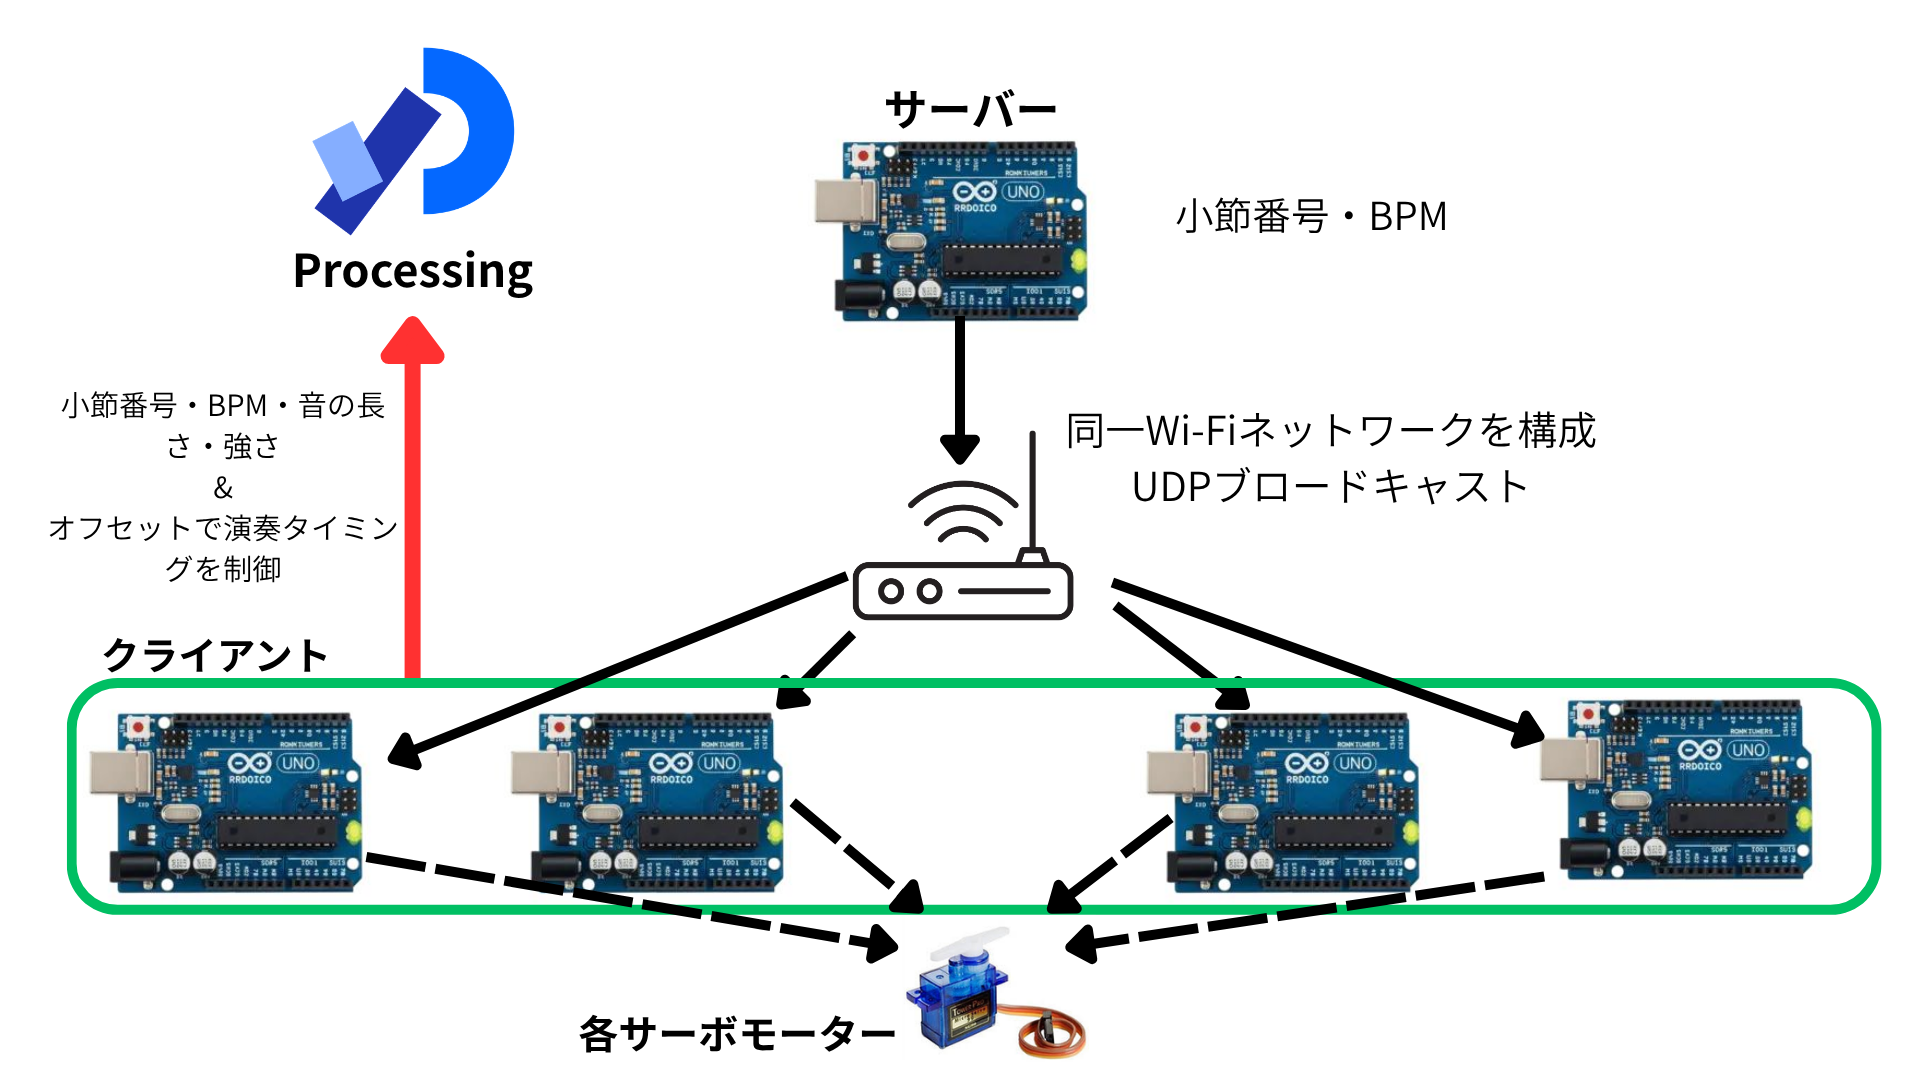
\includegraphics[width=0.8\linewidth]{fig/システム全体構成図.png}
    \caption{システム全体の構成}
    \label{fig:overview}
\end{figure}

各クライアントが担当する楽器の発音は，クライアントに接続されたPC上のProcessingが行う．各クライアントは，
譜面データから読み出した音符の周波数，発音する長さ，強さ，およびテンポをシリアル通信によってProcessingへ送信する．
Processingは受信した情報をもとに楽器音源を合成し，スピーカから再生する．このように，サーバからクライアントへは
Wi-Fiを介して小節番号とテンポが送信され，各クライアントからProcessingへはシリアル通信を介して個々の音符の情報が
送信されるという二段階の信号の流れによって，システム全体の演奏が実現される．
また，各クライアントは受信した小節番号に基づいてサーボモータを駆動し，演奏に同期した人形の動作を行う．

\subsection{通信・同期機能}
% 1章の独自性に対応する中核。サーバ：BPMから小節タイミング算出→UDPブロードキャスト／
% クライアント：受信→内部タイマで自律補間／1バイトのバイナリ設計／再送なしのフェイルセーフ
% ※原理・方式レベルで。コードや閾値などの実装詳細は3節へ
通信・同期機能は，サーバが送信する演奏位置とテンポの情報をクライアントが受信し，各クライアントの演奏の
タイミングを制御する機能である．同期通信の構成を図\ref{fig:sync}に示す．サーバには2つのスイッチが接続されており，
一方を押すとテンポが増加し，他方を押すとテンポが減少する．これにより，演奏中にテンポをリアルタイムで変更できる．
サーバは，現在のテンポと演奏中の小節番号を1バイトのデータとしてUDPでブロードキャストする．クライアントは
受信したデータの値によってその種別を判別し，一定値以上であればテンポ，それ未満であれば小節番号として扱う．
\begin{figure}[h]
    \centering
    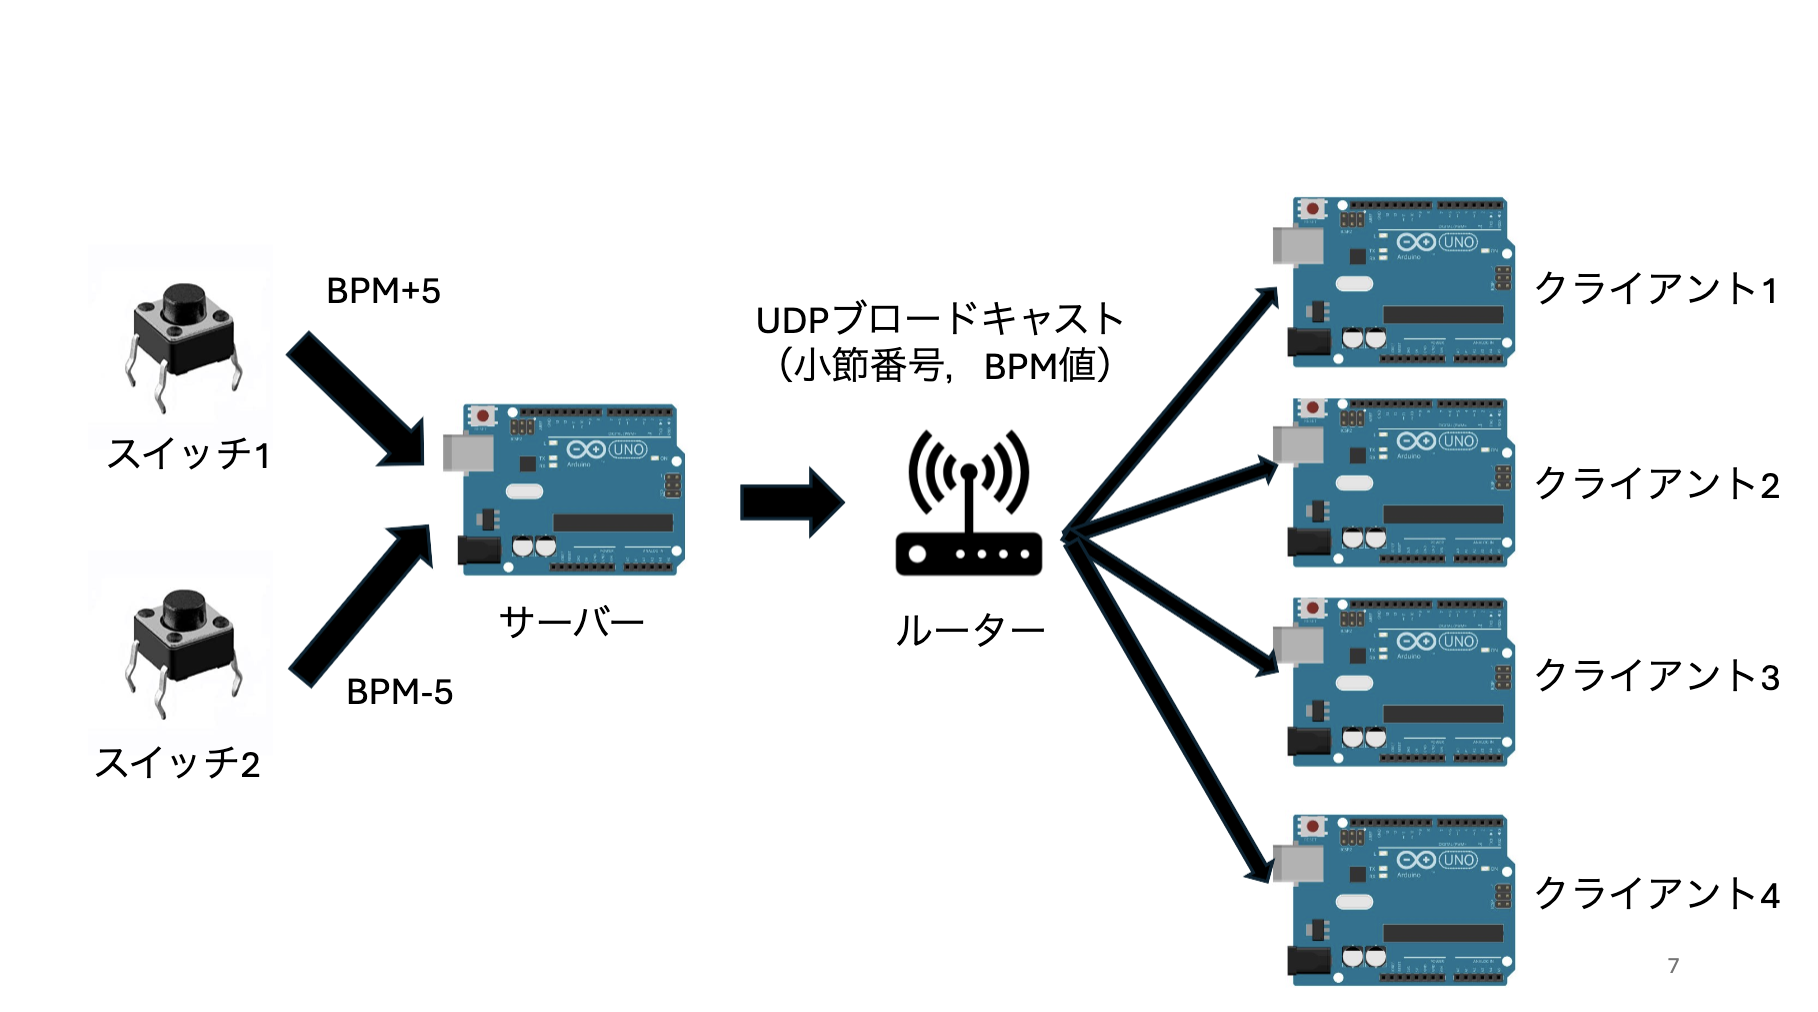
\includegraphics[width=0.8\linewidth]{fig/通信構成図.png}
    \caption{同期通信の構成}
    \label{fig:sync}
\end{figure}

テンポを受信したクライアントは，そのテンポから基準となる4分音符の長さを算出し，以降の演奏の時間基準とする．
小節番号を受信したクライアントは，あらかじめ保持している譜面データからその小節に含まれる音符を先頭から順に
読み出し，各音符の相対的な長さと基準音符長から求めた間隔で，音符の情報をProcessingへ順次送信する．
これにより，サーバが小節単位の位置情報のみを送信し，各クライアントが自身のもつ譜面データに基づいて
小節内の演奏を自律的に進める構成となっている．

また，各クライアントは輪唱を実現するためのオフセットを保持しており，受信した小節番号にオフセットを加えることで
自身の演奏開始位置をずらす．これにより，同一の譜面を複数のクライアントが時間差で演奏し，輪唱として
成立させている．

\subsection{音源の生成・再生機能}
% トロンボーン：波形合成による音色・音階の生成／カスタネット：打楽器音の波形と特有のノイズ
% ※詳細（波形・周波数の実測など）は3節・4節へ
楽器音源の生成・再生機能は，クライアントから送信された音符の情報をもとに，PC上のProcessingが楽器の音を
合成して再生する機能である．Processingは，クライアントからシリアル通信で受信した周波数，発音する長さ，強さ，
およびテンポを解釈し，指定された周波数の音を，その楽器に応じた音色で，指定された長さだけ発音する．

各楽器の音色は，実際の楽器の音響的な特徴を反映するように設計した．例えば，
トロンボーンは音高の明確な持続音を発する楽器であるため，加算合成によって
その音色を再現した．一方，カスタネットは音高を持たない打楽器であり，特定の周波数帯に集中した打撃音を
再現した．これらの音源の具体的な設計と実装については\ref{sec:impl}章で述べる．

\subsection{物理演出機能}
% 人形の駆動機構と，音に同期させる仕組み
物理演出機能は，演奏に合わせて楽器を持った人形を動作させ，視覚的な演出を行う機能である．各クライアントArduinoには
サーボモータが接続されており，人形の腕などの可動部を駆動する．クライアントは，受信した小節番号に基づいて
その小節で演奏すべき動作のタイミングを求め，音の発生に同期してサーボモータを動かす．これにより，人形が
楽器を演奏しているように見せる．

また，各クライアントはテンポの変化を受信した際に，人形に演奏以外の動作を行わせる．これにより，楽曲の
進行に合わせた人形の反応を表現する．人形は演奏する楽器に応じて異なる動作を行い，楽器ごとの演奏の
様子を表現する．ピアノの場合，両手で鍵盤を叩くような動作を行い，トロンボーンの場合は楽器をベルアップさせて下げる動作を繰り返す．
ヴァイオリンは，弓を楽器に当ててさらに口が開くような動作を行い，カスタネットは両手でカスタネットを叩く動作を行う．
カスタネットは，サーバー側のテンポ変化が起きると頭が回転するという動作も行う．
\section{システム実装}
\subsection{チーム構成と役割分担}
本プロジェクトは，6名(近藤・関屋・岩波・須磨・木村・仲里)のチームで実施した．
本システムでは，同期通信機能・楽器音源の生成・再生機能・人形の物理演出機能の3つの機能が必要であり，チームメンバはそれぞれの担当を分担した．
このチームでは，機能ごとにタスクを担当するのではなく，細かい成果物ごとに担当を分担する方式を採用した．
特に，ProcessingやArduinoといったプログラムはハッカソン1の学生が主体となり，ハッカソン2の学生に
そのレビュー及び，手の回らない部分の実装を依頼するという形で，チーム内での役割分担を行った．
なお，本システムのサーバおよびクライアントはいずれもArduinoで実装されており，主要な関数は
サーバ側とクライアント側に分けられる．

\vspace{1zh}\noindent
\textbf{［サーバ側］}

\textbf{Bar\_control()関数}\quad 小節番号を送信する関数である．前回の送信から一定の間隔が経過するたびに
小節番号を1つ進め，その値をUDPでブロードキャスト送信する．小節番号は0から39までの範囲で循環させる．
フローチャートを図\ref{fig:bar_control}に示す．

\textbf{BPM\_control()関数}\quad テンポを変更する関数である．テンポを増減する2つのスイッチの押下を検出し，
上限・下限の範囲内でテンポを5ずつ増減させる．テンポの変更後，最後にスイッチが押されてから一定時間が
経過した時点で，変更後のテンポをUDPで送信する．これにより，スイッチを連続して押した場合でも送信が
1回にまとめられる．フローチャートを図\ref{fig:bpm_control}に示す．

\textbf{detectPress()関数}\quad スイッチの押下を検出する関数である．スイッチの読み値には接点の機械的な
振動によるチャタリングが生じるため，読み値が一定時間安定して初めて状態の変化を確定する．これにより，
1回の押下が複数回として誤検出されることを防ぐ．フローチャートを図\ref{fig:detect_press}に示す．

\vspace{1zh}\noindent
\textbf{［クライアント側］}

\textbf{Parse\_data()関数}\quad 受信データの種別を判別する関数である．サーバから送られる1バイトのデータは
小節番号とテンポのいずれかであり，その値が一定値以上であればテンポ，それ未満であれば小節番号として扱う．
小節番号の場合は，各クライアントに固有のオフセットを加えて自身の演奏位置を求める．フローチャートを
図\ref{fig:parse_data}に示す．

\textbf{BPM\_update()関数}\quad テンポから演奏の時間基準を求める関数である．テンポを受信した際に，
基準となる4分音符の長さをミリ秒単位で算出し，以降の演奏タイミングの基準とする．フローチャートを
図\ref{fig:bpm_update}に示す．

\textbf{Performance()関数}\quad 演奏を進める関数である．受信した小節番号に対応する音符を，あらかじめ
保持している譜面データから先頭から順に読み出す．各音符の周波数，発音する長さ，強さ，およびテンポを
シリアル通信でProcessingへ送信し，音符の長さに応じた間隔をおいて次の音符へ進む．フローチャートを
図\ref{fig:performance}に示す．

% ===== サーバ側 =====
\begin{figure}[H]
  \begin{center}
    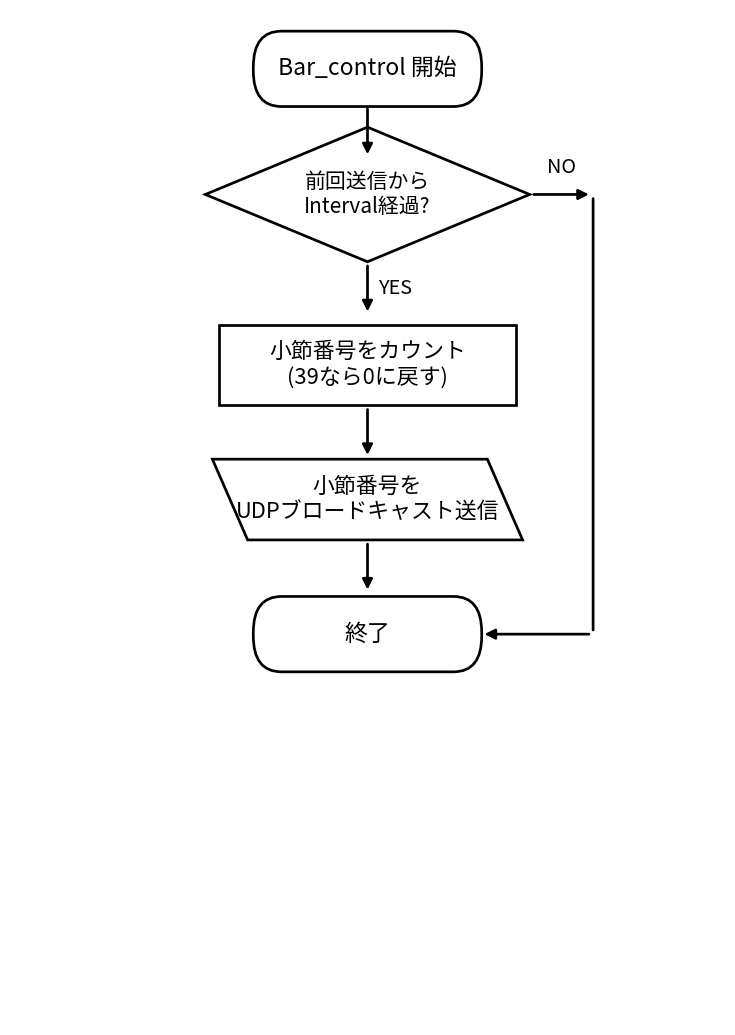
\includegraphics[width=0.55\linewidth]{fig/fc_bar_control.png}
  \end{center}
  \caption{Bar\_control()関数のフローチャート}
  \label{fig:bar_control}
\end{figure}

\begin{figure}[H]
  \begin{center}
    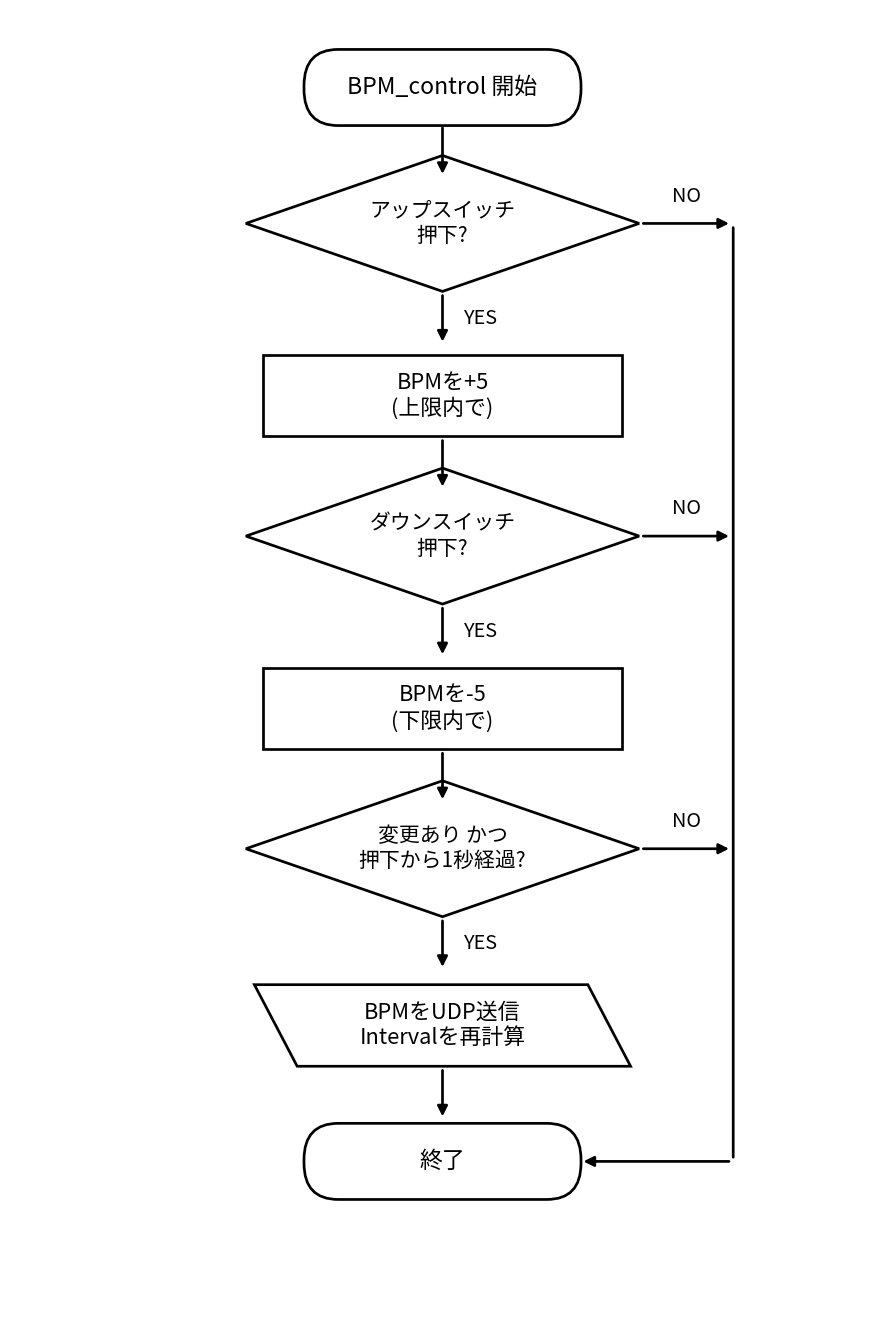
\includegraphics[width=0.6\linewidth]{fig/fc_bpm_control.png}
  \end{center}
  \caption{BPM\_control()関数のフローチャート}
  \label{fig:bpm_control}
\end{figure}

\begin{figure}[H]
  \begin{center}
    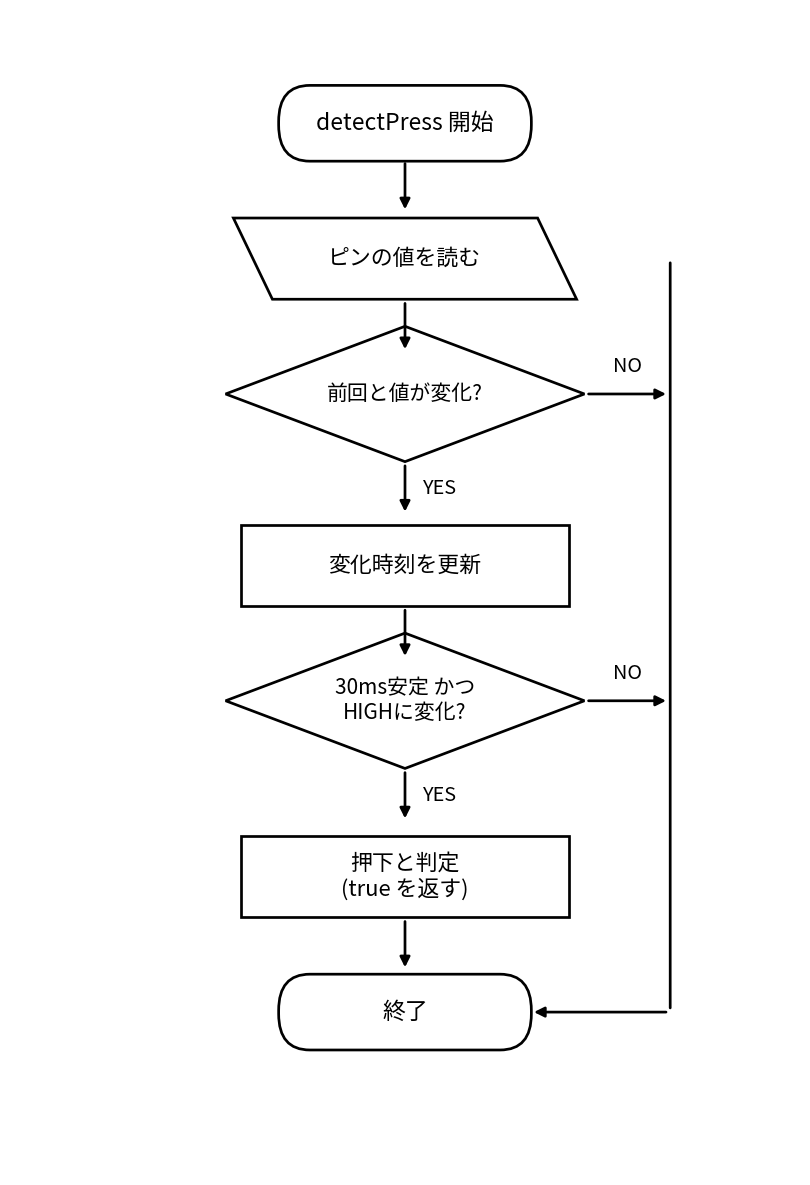
\includegraphics[width=0.55\linewidth]{fig/fc_detect_press.png}
  \end{center}
  \caption{detectPress()関数のフローチャート}
  \label{fig:detect_press}
\end{figure}

% ===== クライアント側フローチャート =====
\begin{figure}[H]
  \begin{center}
    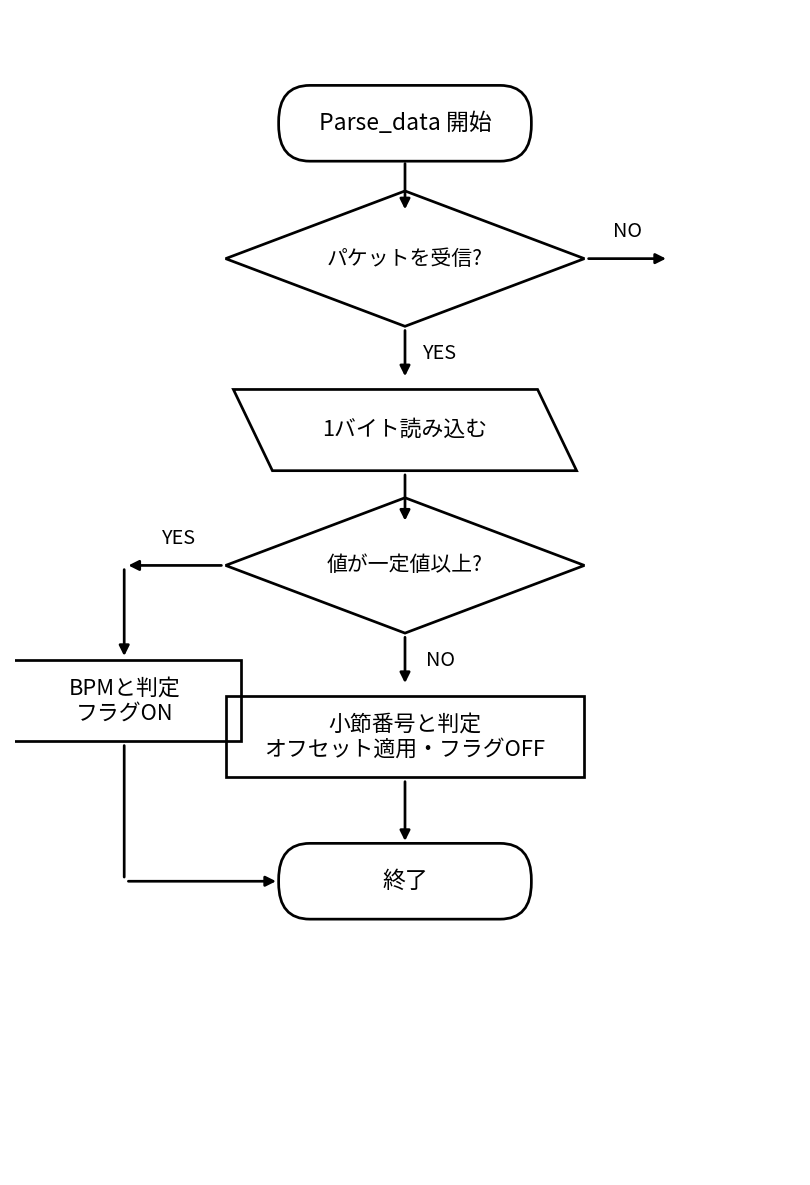
\includegraphics[width=0.55\linewidth]{fig/fc_parse_data.png}
  \end{center}
  \caption{Parse\_data()関数のフローチャート}
  \label{fig:parse_data}
\end{figure}

\begin{figure}[H]
  \begin{center}
    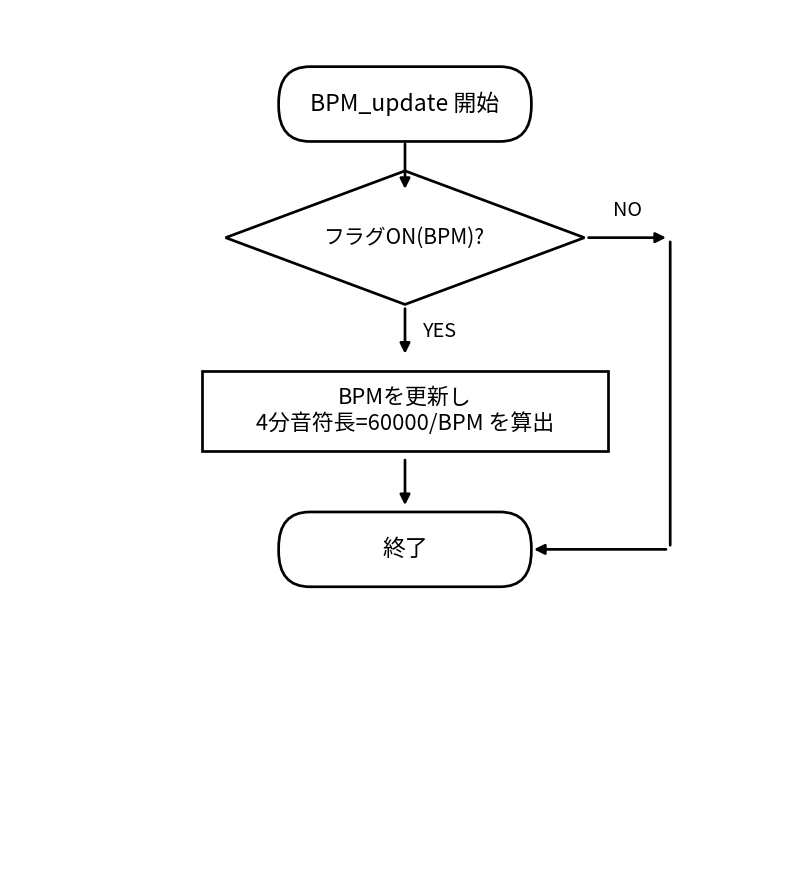
\includegraphics[width=0.5\linewidth]{fig/fc_bpm_update.png}
  \end{center}
  \caption{BPM\_update()関数のフローチャート}
  \label{fig:bpm_update}
\end{figure}

\begin{figure}[H]
  \begin{center}
    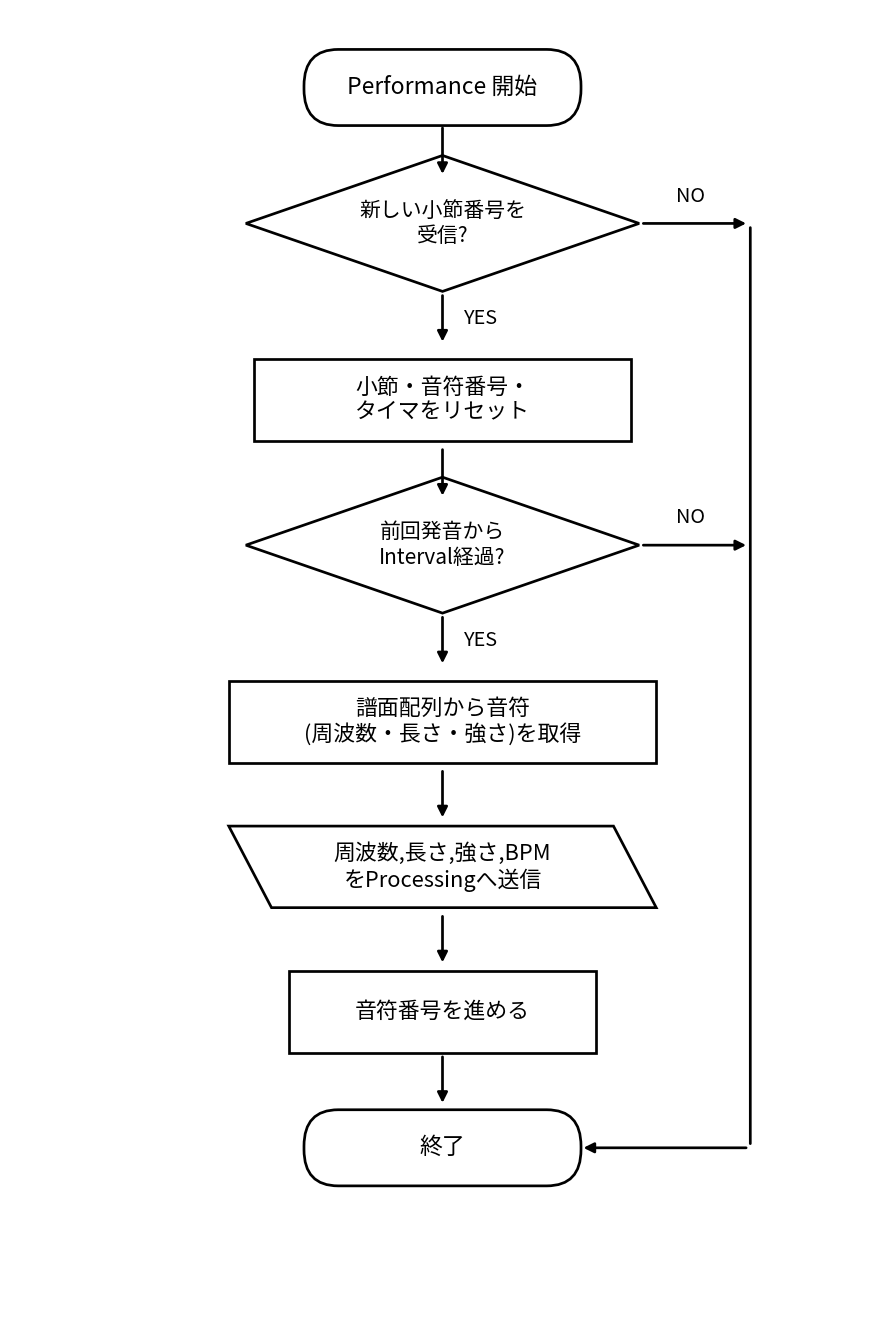
\includegraphics[width=0.55\linewidth]{fig/fc_performance.png}
  \end{center}
  \caption{Performance()関数のフローチャート}
  \label{fig:performance}
\end{figure}


\begin{figure}[H]
    \begin{center}
    \resizebox{\linewidth}{!}{%
    \begin{ganttchart}[y unit title=0.4cm,
    y unit chart=0.5cm,
    vgrid,hgrid,
    title label anchor/.style={below=-1.6ex},
    title left shift=.05,
    title right shift=-.05,
    title height=1,
    title/.append style={fill=yellow!10},
    progress label text={},
    bar height=0.7,
    group right shift=0,
    group top shift=.6,
    group height=.3]{1}{24}
    %labels
    \gantttitle{8 Weeks}{24} \\
    \gantttitle{W1}{3}
    \gantttitle{W2}{3}
    \gantttitle{W3}{3}
    \gantttitle{W4}{3}
    \gantttitle{W5}{3}
    \gantttitle{W6}{3}
    \gantttitle{W7}{3}
    \gantttitle{W8}{3}\\
    %===== 実装フェーズ =====
    \ganttgroup{実装フェーズ}{2}{17} \\
    \ganttbar[bar/.append style={fill=blue!35}]{サーバ・クライアント実装（仲里・岩波）}{2}{11} \\
    \ganttbar[bar/.append style={fill=green!35}]{ピアノ音源（木村）}{2}{9} \\
    \ganttbar[bar/.append style={fill=red!55}]{トロンボーン音源（近藤）}{2}{9} \\
    \ganttbar[bar/.append style={fill=green!35}]{ヴァイオリン音源（仲里）}{9}{15} \\
    \ganttbar[bar/.append style={fill=red!55}]{カスタネット音源（近藤）}{9}{14} \\
    \ganttbar[bar/.append style={fill=orange!40}]{サーボ駆動・エンタメ（木村・関屋）}{2}{17} \\
    \ganttbar[bar/.append style={fill=red!55}]{トロンボーン・カスタネット人形製作（近藤 他）}{11}{16} \\
    \ganttbar[bar/.append style={fill=gray!30}]{ステージ製作（須磨・岩波）}{14}{22} \\
    %===== テストフェーズ =====
    \ganttgroup{テストフェーズ}{5}{24} \\
    \ganttbar[bar/.append style={fill=red!55}]{各楽器の音確認・演奏テスト（近藤・木村・仲里）}{5}{24} \\
    \ganttbar[bar/.append style={fill=gray!30}]{同期・エンタメ動作テスト（仲里・木村・関屋・岩波）}{11}{22} \\
    \ganttbar[bar/.append style={fill=red!55}]{演奏テスト（全員）}{18}{24}
    \end{ganttchart}%
    }
    \end{center}
    \caption{開発スケジュール}
    \label{gantt1}
\end{figure}
図\ref{gantt1}に，開発スケジュールを示す．
まず，サーバー・クライアントの実装は仲里・岩波が担当し，サーバーの同期通信機能を実装した．
次に，Processing上での楽器音源の生成は，それぞれトロンボーンとカスタネットの音色作成を近藤が担当し，ピアノの音色作成を木村が担当した．ヴァイオリンの音色作成は仲里が担当した．
人形のサーボモータ駆動を含むエンタメ部分の実装は木村・関屋が主に担当し，後に人形の
サーボモータ接合部の実装は近藤と仲里で手伝った．
人形を配置するステージの作成は須磨・岩波が担当した．
テストフェーズでは，各楽器の音確認・演奏テストを近藤・木村・仲里が担当し，サーボモータの動作確認テストは木村と関屋が主に担当した．
同期テストはサーバとクライアントの実装を行った仲里と岩波が担当し，最終的な演奏テストは
全員で実施した．

\subsection{報告者の担当範囲と技術的課題}
報告者は，トロンボーンおよびカスタネットの音源をProcessing上で実装した．
他にも後付の作業として人形作成が加わったが，そちらは物理的な作業であり，報告者の専門分野ではないため，本報告書では主に音源の実装について書く．
音源は，クライアントから送信される音符の周波数をもとに，Minimライブラリを用いて波形を合成することで生成する．

トロンボーンの音源を実装するにあたり，まず単純な波形を用いて音を合成した．しかし，矩形波や
単一のオシレータ(一定周期の波形を出力する発振器)による波形では，生成される音は電子的なブザー音のように聞こえ，実際のトロンボーンの
音とは大きく異なるものであった．実物のトロンボーンは，基本周波数に加えて多くの倍音を含み，また
音の立ち上がりや減衰にも特有の変化を持つ．単純な波形ではこれらの特徴が再現されないため，
トロンボーンらしい音色を得ることが課題となった．

カスタネットは，トロンボーンとは異なる種類の課題を持つ．実際のカスタネットの音の波形を
図\ref{fig:castanet_real}に示す．図から，打撃の瞬間に振幅が最大となり，その後急速に減衰していること，
および波形が正弦波のような規則的な周期を持たず，不規則に振動していることが読み取れる．
\begin{figure}[H]
  \begin{center}
    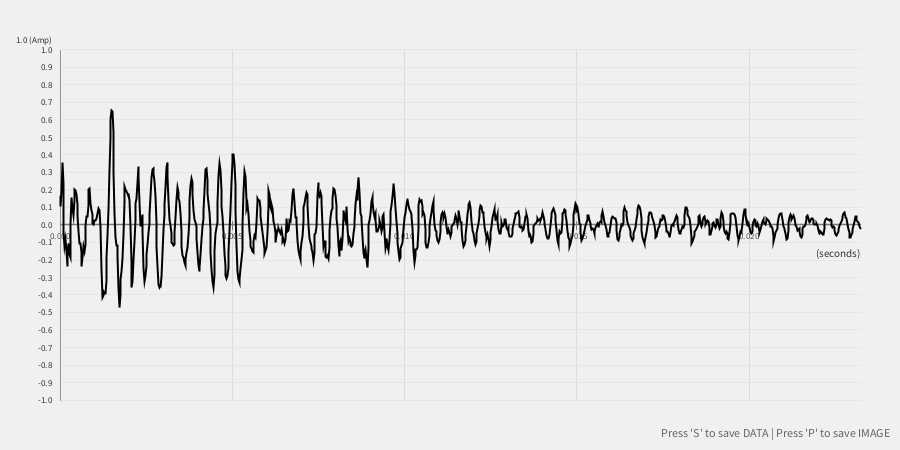
\includegraphics[width=0.8\linewidth]{fig/castanet_real.png}
  \end{center}
  \caption{実際のカスタネットの音の波形}
  \label{fig:castanet_real}
\end{figure}
一方，オシレータは周期的な波形を出力するため，明確な基本周波数を持ち，音程のある音として知覚される．
これは，図\ref{fig:castanet_real}に示したカスタネットの不規則な波形とは根本的に異なる．そのため，
音程を持たず，不規則な打撃音として聞こえるカスタネットの音を，オシレータを基本とするMinimの枠組みで
いかに合成するかが課題となった．

\subsection{予備実験と設計値の決定}
音源の各パラメータは，実測から一意に定まるものではなく，実際の楽器の音に近い聴感が得られるように
調整して決定する必要がある．そこで，Processing上で合成音の波形および周波数成分を確認しながら，
実際の楽器音と聴き比べる予備実験を繰り返し，各設計値を決定した．

トロンボーンの音源では，波形テーブルの倍音構成に加え，音色を整えるためのフィルタおよびエンベロープの
パラメータを調整した．波形テーブルには高次の倍音まで含まれており，そのままでは電子的で硬い音となる．
そこで，遮断周波数1200\,Hzのローパスフィルタを適用し，高域成分を抑えることで管楽器らしい柔らかい音色に
近づけた．また，音の立ち上がりが急峻すぎると機械的な印象となるため，立ち上がり時間を0.08\,秒，減衰時間を
0.05\,秒，持続レベルを0.8，余韻を0.3\,秒とするエンベロープを設定し，管楽器の発音に近い緩やかな立ち上がりと
した．さらに，発音直後に基準周波数の0.96倍から0.12\,秒かけて基準周波数へ移行させることで，金管楽器に
みられる発音時のわずかなピッチの揺れを再現した．設計値を表\ref{tab:trombone_params}に示す．これらの値は
合成音を試聴しながら段階的に決定した．

\begin{table}[H]
  \centering
  \caption{トロンボーン音源の設計値}
  \label{tab:trombone_params}
  \begin{tabular}{ll}
    \hline
    パラメータ & 設計値 \\
    \hline
    ローパスフィルタ遮断周波数 & 1200\,Hz \\
    フィルタのレゾナンス & 0.2 \\
    立ち上がり時間（Attack） & 0.08\,秒 \\
    減衰時間（Decay） & 0.05\,秒 \\
    持続レベル（Sustain） & 0.8 \\
    余韻（Release） & 0.3\,秒 \\
    発音時のピッチ変化 & 基準の0.96倍 $\rightarrow$ 基準（0.12\,秒） \\
    \hline
  \end{tabular}
\end{table}

カスタネットの音源では，打撃音を構成する3つの成分について，中心周波数，フィルタ特性，および減衰時間を
調整した．各成分はノイズを帯域通過フィルタに通して生成するため，フィルタの中心周波数と帯域幅によって
音の質感が決まる．木の胴鳴りに相当する主成分の中心周波数を1000〜2600\,Hzの範囲に設定し，これを基準として
表面の硬い打撃音を約2500〜3600\,Hz高い帯域に，高域の乾いた成分を約4200〜5200\,Hz高い帯域に配置した．
各成分の減衰時間は，打撃音の余韻が短く自然に減衰するように設定し，胴鳴り成分の減衰を0.060\,秒とやや長く，
表面の打撃音を0.007\,秒，高域成分を0.018\,秒と短くした．いずれの成分も持続レベルを0とし，持続音を持たない
打楽器の特性を再現した．設計値を表\ref{tab:castanet_params}に示す．

さらに，実際のカスタネットが打つたびに異なる音になることを再現するため，各成分の中心周波数に発音ごとに
$\pm90$\,Hzの揺らぎを与え，振幅も0.80〜1.05倍の範囲で変動させた．これらの値は，波形および周波数成分の
確認と聴感評価の双方から決定した．

\begin{table}[H]
  \centering
  \caption{カスタネット音源の各成分の設計値}
  \label{tab:castanet_params}
  \begin{tabular}{lcccc}
    \hline
    成分 & 中心周波数 & レゾナンス & 立ち上がり & 減衰 \\
    \hline
    表面の硬い打撃音 & 主成分 $+$ 約3000\,Hz & 0.65 & 0.5\,ms & 7\,ms \\
    木の胴鳴り & 1000〜2600\,Hz & 0.85 & 1\,ms & 60\,ms \\
    高域の乾いた成分 & 主成分 $+$ 約4700\,Hz & 0.55 & 0.5\,ms & 18\,ms \\
    \hline
  \end{tabular}
\end{table}

\subsection{その他の実装}
また音色作成以外の実装として，人形の物理制作・カスタネット用clientの変更を行った．

人形制作に関しては，楽器の模型を作り，サーボモータで動く人形の腕で楽器を演奏するように
段ボールやテープを用いて制作した．

カスタネット用clientの変更に関しては，その他の楽器トロンボーン・ピアノ・ヴァイオリンで
共通で使用しているクライアントプログラムであるclient.inoを，カスタネット用に変更した．
client.inoでは，音符の周波数・長さ・強さをProcessingに送信する処理が行われているが，
カスタネットは音程を持たないため，音の高さを表す周波数の情報は本来不要である．そこで，
他の楽器が音階（262〜880\,Hz）を音符ごとに切り替えていたのに対し，カスタネットでは
発音する周波数を固定値の1800\,Hzとした．これにより，どの打撃に対しても一定の帯域を中心とした
打撃音が生成される．

また，譜面配列についても，音階を並べたメロディではなく，一定の周波数の打撃と休符を
組み合わせた打撃パターンとして構成した．さらに，カスタネットのクライアントは音源の
再生のみを担当し，人形の動作を制御する処理は分離した．

\subsection{担当箇所以外の実装}
\subsubsection{チャタリング対策回路}
サーバでは，テンポを変更するためのスイッチが用いられている．スイッチには接点の機械的な振動による
チャタリングが生じるため，これを除去する必要がある．チャタリングの除去はソフトウェアで実装することも
可能であるが，本システムでは小節番号の通信におけるリアルタイム性を重視し，サーバの処理量を抑える
ために，ハードウェアによるチャタリング対策を行う．BPM変更スイッチのチャタリング対策回路を
図\ref{fig:debounce}に示す．

\begin{figure}[H]
  \begin{center}
    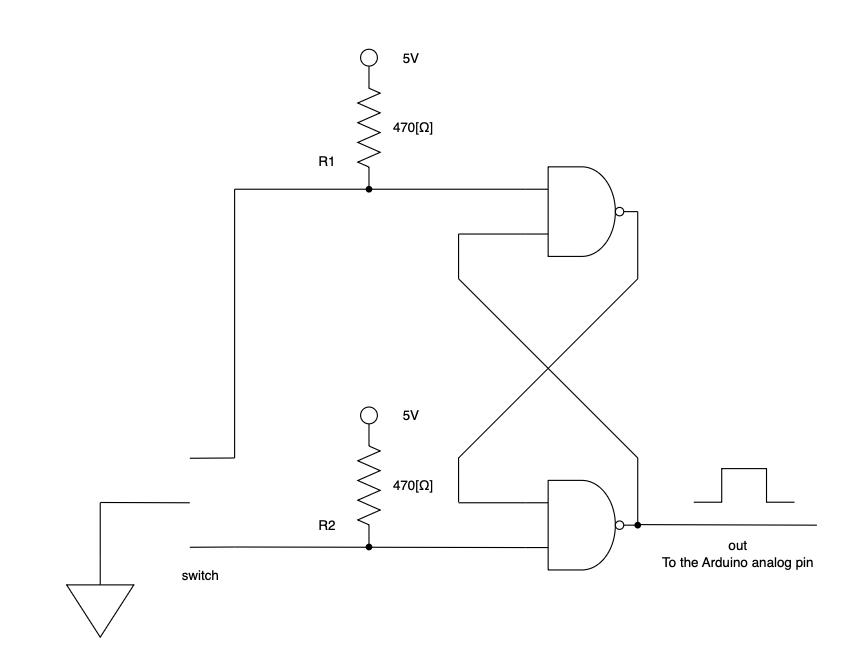
\includegraphics[width=0.7\linewidth]{fig/debounce.png}
  \end{center}
  \caption{BPM変更スイッチのチャタリング対策回路}
  \label{fig:debounce}
\end{figure}

この回路は，2つのNAND素子を交差接続したフリップフロップを用いており，スイッチが切り替わると
回路の状態が保持される．これにより，接点のバウンスによる複数回の信号変化が出力に現れず，
1回の安定した信号が得られる．出力をArduinoのディジタルピンに接続し，\texttt{digitalRead}関数で
スイッチの押下を検出する．BPM変更スイッチはアップ用とダウン用の2つが必要であるため，
この回路もそれぞれに対して実装する．

\subsubsection{サーボモータの接続}
クライアントでは，人形の可動部を駆動するためにサーボモータを用いる．サーボモータとArduinoの接続を
図\ref{fig:servo}に示す．サーボモータの信号線をArduinoのディジタル出力ピンに接続し，5Vを供給して
駆動する．受信した演奏情報に応じてサーボを動作させることで，演奏に同期した人形の動きを実現する．
図\ref{fig:servo}では，サーボモータの電源としてArduinoの5Vを使用しているが，複数のサーボモータを同時に駆動する場合は，外部電源を使用することが望ましい．
実際に，トロンボーン人形を除いたピアノ・カスタネット・ヴァイオリンの３体はそれぞれ2つのサーボモータを使用しており，Arduinoの5Vでは電流が不足するため，外部電源を使用している．
なお，図中ではサーボモータをD9ピンに接続しているが，人形の右腕をD9ピンに，左腕をD11ピンに，頭や口などはD5ピンに接続する設計となっており，
サーボモータの接続ピンは人形ごとに異なる．

\begin{figure}[H]
  \begin{center}
    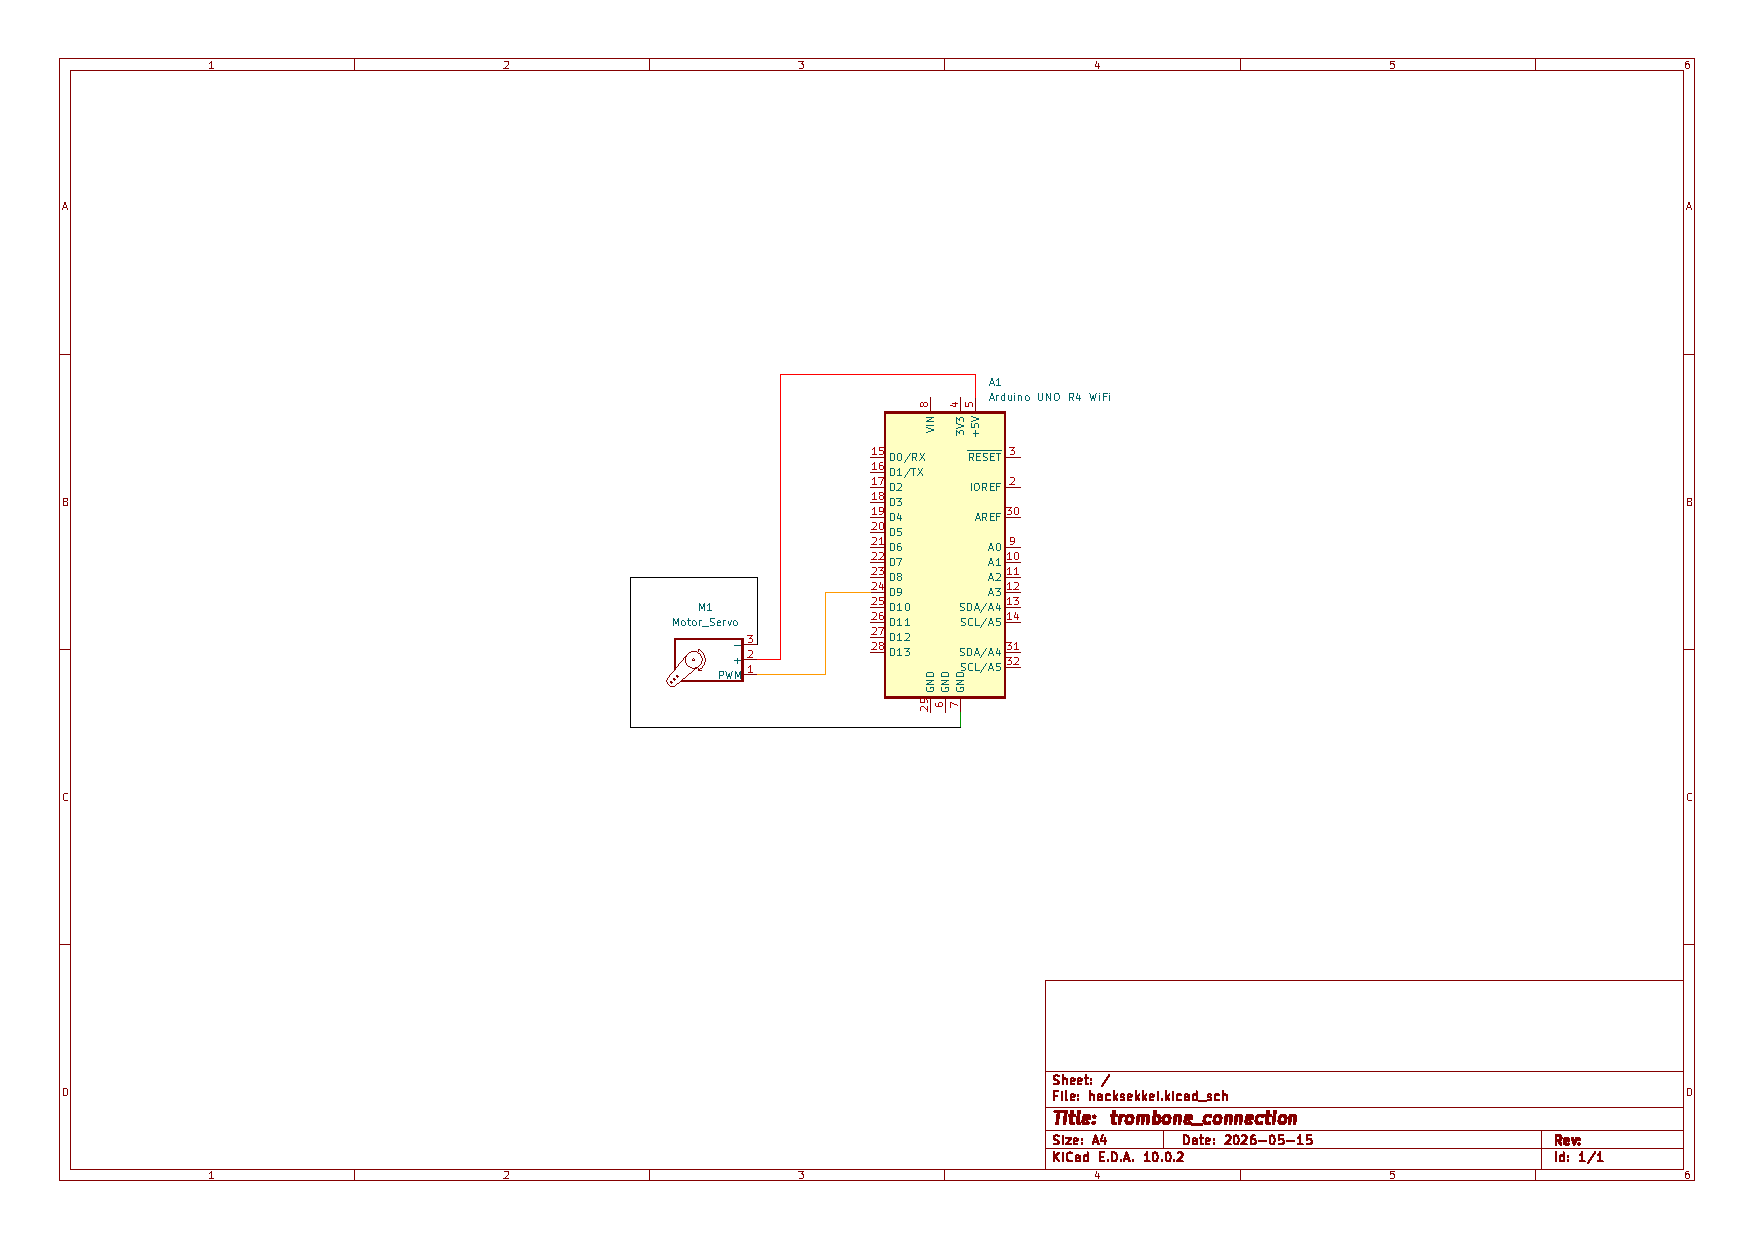
\includegraphics[width=0.7\linewidth]{fig/hacksekkei.pdf}
  \end{center}
  \caption{サーボモータを使用したクライアント部分の回路図}
  \label{fig:servo}
\end{figure}

\subsection{生成AIの活用と検証}
本開発では，音源解析に関するコードの作成に生成AIを活用した．一方で，生成AIが出力する結果は，
その処理内容を理解した上で妥当性を検証する必要がある．本節では，トロンボーンの音源設計における
生成AIの活用とその検証について述べる．

トロンボーンの音色を設計するにあたり，実際のトロンボーンの音に含まれる倍音の構成を参考にすることとした．
そこで，音源のスペクトルから倍音の振幅を抽出するFFT解析のコードの作成を生成AIに依頼し，得られた
コードを用いて解析を行った．当初はこの解析結果を倍音の振幅として波形テーブルに用いた．
しかし，後の検証において，抽出された周波数がいずれも基本周波数の近傍に集中しており，倍音を正しく
抽出できていないことが判明した．原因を確認したところ，生成されたコードはFFTの振幅を単純に大きい順に
並べるものであり，スペクトルのピークを検出する処理を含んでいなかった．そのため，倍音のピークではなく，
基本周波数の1つのピークの近傍にある複数の値を抽出していた．
この問題を踏まえ，解析コードにピーク検出処理（\texttt{scipy.signal.find\_peaks}）を導入し，
ピーク間の最小間隔と卓立度を指定することで，倍音のピークを適切に分離して抽出できるように改善した．
この経験から，生成AIが出力するコードは，処理の内容と結果の妥当性を利用者自身が確認した上で
採用する必要があることを確認した．以降の解析では，公式ドキュメントを参照しながら処理内容を
確認し，生成結果を検証した上で採用する方針を取った．

カスタネットの音源生成においては，これを踏まえて，生成AIに対してFFT解析のコードを作成する際に，ピーク検出処理を含めるように指示した．
更に，Processing上での音色再現についても，減算合成の手法を用いて，FFT解析の結果をもとに各成分の中心周波数・減衰時間・フィルタ特性を調整するコードを生成AIに作成させた．
導入する以前の音色と比較すると，明らかにより実際のカスタネットの音に近い音色が得られ，
その他の問題が発生しないことを確認し，実際のシステムに採用した．

また，楽器の単体テスト用に波形を出力し，周波数を表示するコードを生成AIに作成させ，実際の楽器音と合成音の周波数成分を比較することで，設計値の妥当性を検証した．
コードの中では，もともとinoファイルで定義されている周波数をそのまま使用しているので
正当性は担保されている．それに加え，評価で用いる自己相関法を用いた，理論周波数との相対誤差を算出するコードと，その結果をグラフ化するコードも生成AIに作成させ，
ゼロ交差法も同様に生成AIに作成させた．
\section{評価方法と結果}
\subsection{評価方法}
報告者が担当した楽器音源について，各楽器の音確認テストと演奏テストの2つを実施した．音確認テストでは
客観評価と主観評価の両面から，演奏テストでは発音の完遂性から評価を行った．

\subsubsection{音確認テスト}
音確認テストでは，Processingによって生成される音が，各楽器の物理的特性に基づく理論的な周波数を
正確に再現できているかを検証する．客観評価では，合成音の波形を取得し，その基本周波数を測定して
目標とする音高の理論周波数と比較する．基本周波数の測定には，自己相関法およびゼロ交差法を用いた．
測定された周波数$f_\mathrm{meas}$と理論周波数$f_\mathrm{ref}$との相対誤差を次式で定義する．
\begin{equation}
  \varepsilon = \frac{|f_\mathrm{meas} - f_\mathrm{ref}|}{f_\mathrm{ref}} \times 100 \quad [\%]
\end{equation}
評価基準は，相対誤差$\varepsilon$が$\pm1.0$\,\%以内であることとした．

主観評価では，被験者に各楽器の音を提示し，「意図された楽器を正しく識別できる」および「音の減衰や
響きが自然である」の2項目について5段階（5:非常にそう思う〜1:全くそう思わない）で評価を得た．
被験者数を$N$，各被験者の評価値を$S_i$としたとき，平均評価値$S_\mathrm{avg}$を次式で定義する．
\begin{equation}
  S_\mathrm{avg} = \frac{1}{N}\sum_{i=1}^{N} S_i
\end{equation}
評価基準は，平均評価値$S_\mathrm{avg}$が4.0以上であることとした．

\subsubsection{演奏テスト}
演奏テストでは，Arduinoによる譜面配列の参照からProcessingでの発音に至るまで，実曲の演奏において
システムが正常に機能するかを検証する．複数の小節にわたる連続的な演奏を対象とし，リズムのずれや
音の欠落が発生しないかを確認する．評価指標として，正常に発音された音符数の割合を示す発音成功率
$R_\mathrm{success}$を次式で定義する．
\begin{equation}
  R_\mathrm{success} = \frac{\text{正常発音数}}{\text{全音符数}} \times 100 \quad [\%]
\end{equation}
ここで正常発音数は，譜面配列の音符情報が欠落なくProcessingへ送信され，設計通りの周波数で発音された
回数を示す．評価基準は，発音成功率$R_\mathrm{success}$が100\,\%であることとした．

\subsection{客観評価の結果}
各楽器音源の客観評価の結果を表\ref{tab:objective}に示す．また，各楽器について，実際の楽器の音の波形と
合成音の波形を取得し，比較を行った．

報告者が担当したトロンボーンでは，目標とするC3（理論周波数131.0\,Hz）に対し，測定された周波数は
131.05\,Hz，音高の誤差は$+0.3$\,centであり，誤差$\pm1.0$\,\%以内という基準を満たした．
トロンボーンの実際の音の波形を図\ref{fig:trom_real}に，合成音の波形を図\ref{fig:trom_record}に示す．
実際の波形は，基本周期ごとに鋭いピークを持つ倍音の豊かな波形を示している．合成音の波形も同様に
周期的な波形を示しており，基本周波数が再現できていることが確認できる．一方で，合成音は実際の波形に
比べて振幅が小さく，波形の細部の複雑さも少ない．これは，後述するように音源の音量が小さいこと，
および倍音構成が実際の楽器と完全には一致していないことによると考えられる．

カスタネットについては，音程を持たない打楽器であるため，周波数の誤差ではなく波形の特性で評価した．
カスタネットの実際の音の波形を図\ref{fig:cast_real}に，合成音の波形を図\ref{fig:cast_record}に示す．
実際の波形は，打撃の瞬間に振幅が最大となり，その後不規則に振動しながら急速に減衰している．
合成音の波形も，立ち上がり直後に振幅が最大となり，約20\,msで減衰する打撃音特有の波形を示した．
ピーク振幅は0.17であり，音程を持たない打撃音として妥当な波形が得られたと判断した．

また，参考として，他のメンバーが担当したピアノおよびヴァイオリンについても客観評価を行い，
いずれも理論周波数との誤差$\pm1.0$\,\%以内を満たした．さらに，すべての楽器について実曲演奏テストを
行い，全音符が欠落なく発音され，発音成功率は100\,\%であった．

\begin{table}[H]
  \centering
  \caption{楽器音源の客観評価の結果}
  \label{tab:objective}
  \begin{tabular}{lccc}
    \hline
    楽器 & 目標周波数 & 測定結果 & 判定 \\
    \hline
    ピアノ & C4（261.6\,Hz） & 261.67\,Hz（$+0.3$\,cent） & 達成 \\
    トロンボーン & C3（131.0\,Hz） & 131.05\,Hz（$+0.3$\,cent） & 達成 \\
    ヴァイオリン & C4（261.6\,Hz） & 263.15\,Hz（$+0.58$\,cent） & 達成 \\
    カスタネット & --- & 約20\,msで減衰する打撃波形 & 達成 \\
    \hline
  \end{tabular}
\end{table}

\begin{figure}[H]
  \begin{minipage}{0.5\linewidth}
    \centering
    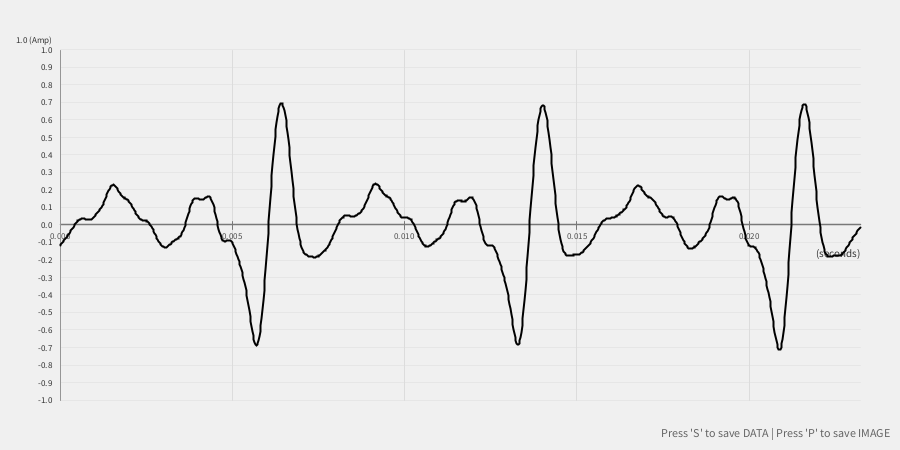
\includegraphics[width=\linewidth]{fig/trombone_real.png}
    \caption{トロンボーン（実物）の波形}
    \label{fig:trom_real}
  \end{minipage}%
  \begin{minipage}{0.5\linewidth}
    \centering
    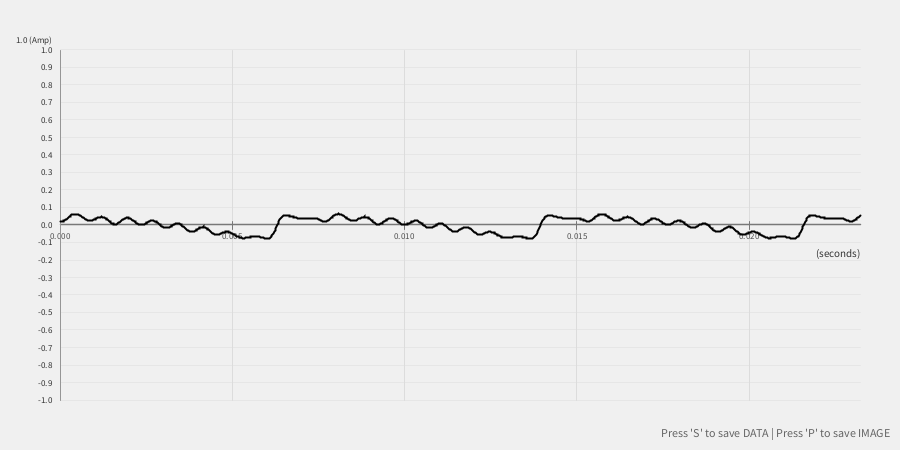
\includegraphics[width=\linewidth]{fig/trombone_record.png}
    \caption{トロンボーン（合成音）の波形}
    \label{fig:trom_record}
  \end{minipage}
\end{figure}

\begin{figure}[H]
  \begin{minipage}{0.5\linewidth}
    \centering
    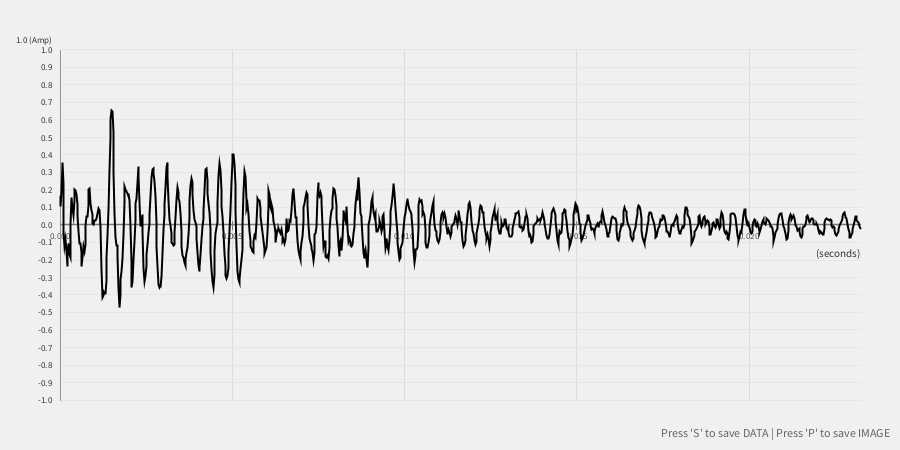
\includegraphics[width=\linewidth]{fig/castanet_real.png}
    \caption{カスタネット（実物）の波形}
    \label{fig:cast_real}
  \end{minipage}%
  \begin{minipage}{0.5\linewidth}
    \centering
    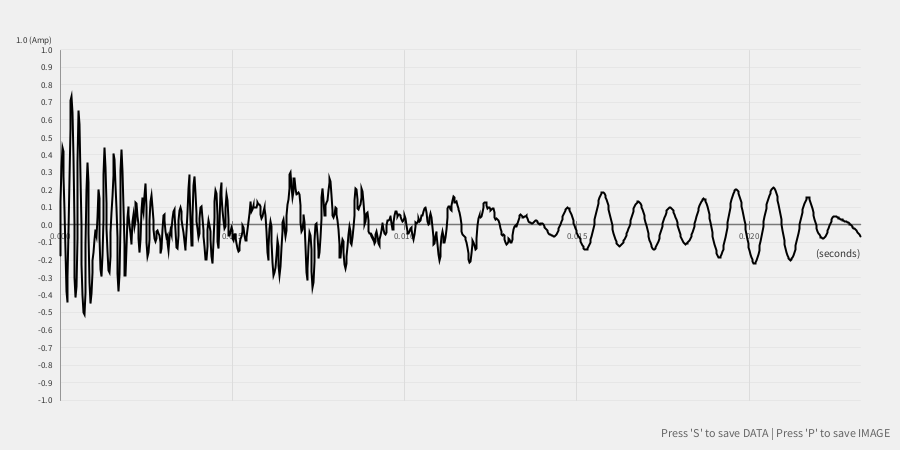
\includegraphics[width=\linewidth]{fig/castanet_record.png}
    \caption{カスタネット（合成音）の波形}
    \label{fig:cast_record}
  \end{minipage}
\end{figure}

\subsection{主観評価の結果}
32名を対象に実施したアンケートによる主観評価の結果を表\ref{tab:subjective}に示す．報告者が担当した
トロンボーンは，作成音3.88，音質3.97であり，全楽器の中で比較的高い評価を得た．カスタネットは
作成音3.44，音質3.81であった．一方で，いずれの楽器も作成音の評価は基準の4.0に達しなかった．
これは，合成音の音量が小さいことや，演奏時のサーボモータの駆動音が影響したためと考えられる．
音質については，トロンボーンをはじめ複数の楽器で3.8以上の評価が得られた．

\begin{table}[H]
  \centering
  \caption{楽器音源の主観評価の結果（$n=32$，5段階）}
  \label{tab:subjective}
  \begin{tabular}{lcc}
    \hline
    楽器 & 作成音 & 音質 \\
    \hline
    ピアノ & 3.56 & 3.97 \\
    トロンボーン & 3.88 & 3.97 \\
    ヴァイオリン & 3.06 & 3.22 \\
    カスタネット & 3.44 & 3.81 \\
    \hline
  \end{tabular}
\end{table}
\section{考察}
\subsection{客観評価と主観評価の乖離}
報告者が担当したトロンボーンおよびカスタネットは，客観評価においては周波数誤差$\pm1.0$\,\%以内という
基準を満たした一方で，主観評価では作成音の平均評価値がいずれも基準の4.0に達しなかった．この乖離に
ついて考察する．

ここで，客観評価と主観評価では測定条件が異なる点に注意する必要がある．客観評価は音源単体で取得した
波形に基づくものであり，音源の周波数特性そのものを評価している．これに対し主観評価は，人形の動作を
含むシステム全体の演奏を提示して行ったものである．したがって，主観評価には音源そのものの音色だけで
なく，演奏環境全体の要因が反映される．

主観評価が伸びなかった要因としては，合成音の音量が実際の演奏環境において十分でなかったこと，および
他楽器と比べ，オクターブを一つ下で設定しているため，音色が低く聞こえ，音量が小さく感じられたことが考えられる．
特にヴァイオリンは高音域で音色的にも目立つ楽器なので，トロンボーンやカスタネットの音が埋もれてしまい，主観評価において低い評価となったと考えられる．
これに関してはピアノでも同様の傾向が見られたため，ヴァイオリンの音が他楽器の音が埋もれる原因となった可能性が高いと思われる．

\subsection{トロンボーンの音色成立の要因}
トロンボーンの音源では，波形テーブルに設定した倍音構成が，実際のトロンボーンの倍音構造を正確に
反映したものではなかった．にもかかわらず，合成音は電子的なブザー音ではなく，
管楽器に近い音色として成立し，主観評価においても音質は3.97と比較的高い評価を得た．この要因について
考察する．

本音源では，オシレータが生成する波形に対し，ローパスフィルタ，ディレイ，および音量エンベロープを
直列に適用している．ローパスフィルタは高次の倍音成分を抑制するため，波形テーブルの倍音構成が
正確でなくとも，過剰な高域成分が除去され，硬い電子音的な質感が緩和される．また，音量エンベロープに
よる緩やかな立ち上がりと減衰は，管楽器特有の発音の印象を与える．これらのことから，本音源の音色は，
波形テーブルの倍音構成そのものよりも，フィルタおよびエンベロープによる後段の処理に強く依存して
決定されていたと考えられる．この結果は，オシレータの倍音設計が不完全な場合でも，フィルタと
エンベロープの設計によって楽器らしい音色を得られる可能性を示している．

\subsection{カスタネットの打撃音合成の有効性}
カスタネットの音源では，オシレータではなくノイズを音源とし，これを帯域通過フィルタと音量エンベロープに
通す構成を採用した．評価の結果，合成音は立ち上がり直後に振幅が最大となり，約20\,msで減衰する打撃音
特有の波形を示した．これは，音程を持たない非調和的な打撃音という，カスタネットの音響的特徴を
再現できたことを示している．オシレータを用いる合成では明確な基本周波数を持つ音となり，打楽器の
質感を再現することが難しいのに対し，ノイズを音源とし帯域通過フィルタで周波数帯を限定する手法は，
打楽器音の合成に有効であったと考えられる．

\subsection{改善案}
以上の評価と考察を踏まえ，今後の改善点を述べる．第一に，主観評価が伸びなかった要因である音量の
不足については，音源の出力レベルを見直すとともに，Processing側でゲインを調整することでの改善が期待される．
第二に，トロンボーンの音色については，実際の楽器の倍音構造をピーク検出によって正確に抽出し，
波形テーブルに反映することで，より実物に近い音色が得られると考えられる．これらの改善により，
客観評価に加えて主観評価においても基準を満たす音源の実現が期待される．
\section{おわりに}
本プロジェクトでは，幼児教育での活用を目的として，複数の楽器が同期して演奏し，あわせて演奏に
同期して動作する人形による視覚的演出を行う分散型の自動演奏システムを開発した．このうち報告者は，
トロンボーンおよびカスタネットの音源の設計と実装を担当した．

トロンボーンの音源では，オシレータによる波形にローパスフィルタ，ディレイ，および音量エンベロープを
適用することで，管楽器に近い音色を合成した．カスタネットの音源では，オシレータではなくノイズを
音源とし，これを帯域通過フィルタと音量エンベロープに通すことで，音程を持たない打撃音を再現した．

評価の結果，客観評価においては，担当したいずれの楽器も理論周波数との誤差が$\pm1.0$\,\%以内という
基準を満たし，実曲の演奏においても発音成功率100\,\%を達成した．一方，主観評価では，作成音の平均
評価値が基準の4.0に達しなかった．これは，合成音の音量や，他の楽器との音量・音域の関係によって，
担当した楽器の音が相対的に埋もれたことが要因と考えられる．また，トロンボーンの音色設計においては，
生成AIを用いた倍音の抽出に誤りがあったものの，フィルタおよびエンベロープによる処理によって，
管楽器に近い音色を得ることができた．

今後の課題として，音源の音量や音量バランスの調整，および実際の楽器の倍音構造を正確に抽出して
波形に反映することが挙げられる．これらの改善により，客観評価に加えて主観評価においても基準を
満たす音源の実現が期待される．本システムは，音と視覚的演出を組み合わせることで，幼児のリズム
教育に活用できる自動演奏システムとしての可能性を示すものである．

\begin{thebibliography}{99}
\bibitem{shigeno2020} 茂野仁美，乳幼児保育におけるリズムへの同期の発達過程に関する文献研究．大阪総合保育大学紀要，(14)，213-226，2019．
\bibitem{takasino} 高橋むつみ，篠田晴男，幼児期におけるリズム知覚と協応動作の発達：音楽活動を通した発達支
援の一助として，茨城大学教育学部紀要(教育科学)，(52)，249-262，2003．
\bibitem{Lazzaro} Lazzaro,J., \& Wawryzynek,J.(2001)."A case for network musical performance."Pro-
ceedings of the 11th international workshop on Network and operating systems support for
digital audio and video (NOSSDAV).
\bibitem{Rottondi} Rottondi, C., Chafe, C., Allocchio, C., \& Sart, A. (2016). ”An Overview on Networked
Music Performance Technologies.” IEEE Access, 4, 8823-8843.
\bibitem{NTPSNTP} D. Mills, J. Martin, J. Burbank and W. Kasch, “Network Time Protocol Version 4:
Protocol and Algorithms Specification,” RFC 5905, Jun. 2010.
\bibitem{PTP} IEEE, “IEEE Standard for a Precision Clock Synchronization Protocol for Networked
Measurement and Control Systems,” IEEE Std 1588-2019 (Revision of IEEE Std 1588-
2008), pp. 1–499, Nov. 2019.
\end{thebibliography}


\appendix
\renewcommand{\thefigure}{A.\arabic{figure}} % 図番号を A.1, A.2 に
\renewcommand{\thetable}{A.\arabic{table}}   % 表番号も変える場合
\renewcommand{\theequation}{\Alph{section}.\arabic{equation}} %式番号をA.1, A.2に

\section{プログラムソース}

\subsection{報告者担当分}
報告者が担当した，トロンボーンおよびカスタネットの音源のソースコードを示す．いずれもProcessingで記述されており，クライアントからシリアル通信で受信した音符の情報をもとに音を合成して再生する．また，合成音の波形を描画し，基本周波数を測定して表示する機能を備える．

\subsubsection{トロンボーンの音源}

\begin{lstlisting}
import processing.serial.*;
import ddf.minim.*;
import ddf.minim.ugens.*;

Serial myPort;
Minim minim;
AudioOutput out;
Waveform currentWaveform;
// --- 表示用変数 ---
String currentNote = "REST";
int currentBpm = -1; // 初期値は未設定にして外部から読み込む
String currentDurationName = "REST";

// 基準音符長（デフォルト: 1.0 = 1拍単位）
float ToneLength = 1.0f;

float[] maxAmp = new float[29];
long lastNoteEndMillis = 0;
float currentToneLengthSec = 0.0f; // 現在鳴っている音の秒数
float currentToneLengthBeats = 0.0f; // 現在鳴っている音の拍数

// --- 周波数計測用 ---
float measuredFreq = 0.0f;   // 自己相関法で計測した基本周波数(Hz)
float displayedFreq = 0.0f;  // 表示用に平滑化した自己相関周波数(Hz)
float measuredZc = 0.0f;     // ゼロ交差法で計測した基本周波数(Hz)
float displayedZc = 0.0f;    // 表示用に平滑化したゼロ交差周波数(Hz)
float displayedPeak = 0.0f;  // 表示用に平滑化したピーク振幅
float AMP_GATE = 0.01f;      // この音量(RMS)未満は無音とみなし計測しない

// 目標周波数：C4(261.63Hz)を1オクターブ下げた値（本システムはfreq/2で発音）
float TARGET_FREQ = 261.63f / 2.0f; // = 130.815 Hz（C3相当）

// --- トロンボーンの特性を反映したクラス ---
class HackInstrument implements Instrument
{
  Oscil wave;
  MoogFilter filter; 
  Delay delay;
  ADSR ampEnv;
  Line freqEnv;
  float baseFreq;
  float maxAmpValue;

  HackInstrument(float frequency, float amplitude, Waveform wf)
  {
    baseFreq = frequency;
    maxAmpValue = amplitude;
    wave = new Oscil(frequency * 0.96f, 1.0, wf);

    filter = new MoogFilter(1200.0f, 0.2f, MoogFilter.Type.LP);
    delay = new Delay(0.2f, 0.3f, true, true);

    // ADSRの引数: (最大音量, アタック秒, ディケイ秒, サステイン比率, リリース秒)
    // 管楽器らしく 0.08秒かけて音が立ち上がり、吹いている間は 80% の音量をキープします
    ampEnv = new ADSR(amplitude, 0.08f, 0.05f, 0.8f, 0.3f);
    
    // 波形の出力を音量エンベロープ（ampEnv）にパッチする
    wave.patch(filter).patch(delay).patch(ampEnv);
    
    freqEnv = new Line();
    freqEnv.patch(wave.frequency);
  }

  void noteOn(float duration)
  {
    ampEnv.noteOn(); // ADSRのトリガー開始
    ampEnv.patch(out); // 出力ポートへ接続
    freqEnv.activate(0.12f, baseFreq * 0.96f, baseFreq);
  }

  void noteOff()
  {
    ampEnv.noteOff(); // 音を消し始める（リリースタイム開始）
    ampEnv.unpatchAfterRelease(out); // 音が完全に消え去った後に自動で接続を解除（ブツ切り防止）
  }
}

void setup()
{
  size(600, 300);
  pixelDensity(1); // 高密度ディスプレイでの自動2倍描画を無効化（従来の見た目に戻す）
  // 日本語が「□（豆腐）」にならないよう、日本語対応フォントを設定する
  textFont(pickJapaneseFont(40));
  textSize(24);
  minim = new Minim(this);
  out = minim.getLineOut();
  out.setGain(2.0);
  currentBpm = loadBpm();
  out.setTempo(currentBpm);
  
  // シリアルポートの初期化処理
  // 利用可能なポートを表示し、Arduino（usbmodem / usbserial）を自動で探して接続する
  printArray(Serial.list());
  String portName = null;
  for (int i = 0; i < Serial.list().length; i++) {
    String s = Serial.list()[i];
    if (s.indexOf("usbmodem") >= 0 || s.indexOf("usbserial") >= 0) {
      portName = s;
      break;
    }
  }
  if (portName != null) {
    myPort = new Serial(this, portName, 115200);
    myPort.bufferUntil('\n');
    println("Serial connected: " + portName);
  } else {
    println("Arduinoのポートが見つかりません。上のリストから手動で指定してください。");
  }
  
  for(int i=0; i<maxAmp.length; i++) maxAmp[i] = 0.15f;
  
  setTromboneWave();
  textSize(24);
}

void setTromboneWave() {
  currentWaveform = WavetableGenerator.gen10(
    4096, 
    new float[] {
      1.0000f, 0.96f, 0.90f, 0.84f, 0.76f, 
      0.72f, 0.71f, 0.63f, 0.57f, 0.56f
    }
  );
}

// BPMを外部から取得する: 環境変数 HCK_BPM または BPM、
// もしくはスケッチの data フォルダに置いた "bpm.txt" の1行目を読み込む。
int loadBpm() {
  // 1) 環境変数
  try {
    String env = System.getenv("HCK_BPM");
    if (env == null) env = System.getenv("BPM");
    if (env != null) {
      env = trim(env);
      if (env.length() > 0) {
        try { return Integer.parseInt(env); } catch (Exception e) {}
      }
    }
  } catch (Exception e) {
    // ignore
  }

  // 2) data/bpm.txt
  try {
    String[] lines = loadStrings("bpm.txt");
    if (lines != null && lines.length > 0) {
      String s = trim(lines[0]);
      if (s.length() > 0) {
        try { return Integer.parseInt(s); } catch (Exception e) {}
      }
    }
  } catch (Exception e) {
    // ファイルが無ければ無視
  }

  // 3) フォールバック
  return 120;
}

void draw() {
  background(0); // 画面を黒で塗りつぶしてリセット（オシロスコープ風）

  // --- オシロスコープ風グリッド（目盛り）と軸の単位を描画 ---
  // 縦方向の拡大率：振幅1.0が gain ピクセルに対応する
  float gain = height * 1.5f;
  // 画面横幅ぶんに相当する時間(ms)＝バッファ長 / サンプリングレート
  float totalMs = out.bufferSize() / out.sampleRate() * 1000.0f;
  drawScopeGrid(gain, totalMs);

  // 出力バッファ（out.mix）の波形を描画（正方向を上＝オシロスコープと同じ向き）
  stroke(0, 255, 120); // 波形の色（緑）
  strokeWeight(1.5f);
  noFill();
  for (int i = 0; i < out.bufferSize() - 1; i++) {
    float x1 = map(i,     0, out.bufferSize(), 0, width);
    float x2 = map(i + 1, 0, out.bufferSize(), 0, width);
    float y1 = height / 2 - out.mix.get(i)     * gain;
    float y2 = height / 2 - out.mix.get(i + 1) * gain;
    line(x1, y1, x2, y2);
  }

  // --- 周波数を計測して画面に表示 ---
  measuredFreq = detectFrequency(out.mix, out.sampleRate());        // 自己相関法
  measuredZc   = detectFreqZeroCross(out.mix, out.sampleRate());    // ゼロ交差法
  float peak   = peakAmplitude(out.mix);                            // ピーク振幅
  if (measuredFreq > 0) {
    // 急な変動を抑えるため指数移動平均で平滑化
    displayedFreq = (displayedFreq <= 0) ? measuredFreq
                                         : displayedFreq * 0.8f + measuredFreq * 0.2f;
    displayedZc   = (displayedZc <= 0 || measuredZc <= 0) ? measuredZc
                                         : displayedZc * 0.8f + measuredZc * 0.2f;
    displayedPeak = displayedPeak * 0.8f + peak * 0.2f;
  } else {
    displayedFreq = 0;
    displayedZc = 0;
    displayedPeak = 0; // 無音
  }
  drawFreqReadout(displayedFreq, displayedZc, displayedPeak);

  // 保存リクエストがあれば、ヒント等を描く前のきれいな画面を保存する
  if (saveRequested) {
    String fn = "capture_" + timestamp() + ".png";
    save(fn); // スケッチフォルダ直下に保存（波形＋周波数のみ）
    lastSavedName = fn;
    savedFlashUntil = millis() + 1500;
    println("画像を保存しました: " + sketchPath(fn));
    saveRequested = false;
  }
}

// オシロスコープ風：薄い目盛りグリッド＋原点を通る太い縦軸/横軸を描画する
void drawScopeGrid(float gain, float totalMs) {
  pushStyle();
  textSize(11);

  float cy = height / 2.0f;      // 振幅0（横軸）のy
  float ox = 2;                  // 時間0（縦軸）のx（左端。太線が見えるよう少し内側）
  float msPerDiv = 5.0f;
  float ampPerDiv = 0.1f;
  float ampMax = cy / gain;      // 画面端に相当する振幅
  int   maxDiv  = (int)(ampMax / ampPerDiv);

  // ===== 1) 薄い目盛りグリッド（背景・控えめ）=====
  strokeWeight(1);
  stroke(38);
  for (float t = 0; t <= totalMs + 0.001f; t += msPerDiv) {   // 時間の縦線
    float x = t / totalMs * width;
    line(x, 0, x, height);
  }
  for (int k = -maxDiv; k <= maxDiv; k++) {                   // 振幅の横線
    if (k == 0) continue;
    float y = cy - k * ampPerDiv * gain;
    line(0, y, width, y);
  }

  // ===== 2) 原点を通る太い軸（はっきり）=====
  stroke(0, 210, 255);   // 水色で目立たせる（波形の緑と区別）
  strokeWeight(2);
  line(0, cy, width, cy);      // 横軸（時間 t：振幅0のライン）
  line(ox, 0, ox, height);     // 縦軸（振幅 A：時間0のライン）

  // 軸上の目盛りマーク（ティック）
  stroke(0, 210, 255);
  strokeWeight(1);
  for (float t = msPerDiv; t < totalMs; t += msPerDiv) {      // 横軸のティック
    float x = t / totalMs * width;
    line(x, cy - 4, x, cy + 4);
  }
  for (int k = -maxDiv; k <= maxDiv; k++) {                   // 縦軸のティック
    if (k == 0) continue;
    float y = cy - k * ampPerDiv * gain;
    line(ox, y, ox + 8, y);
  }

  // ===== 3) 数値ラベル =====
  noStroke();
  textAlign(CENTER, TOP);
  fill(190);
  for (float t = msPerDiv; t < totalMs; t += msPerDiv) {      // 時間[ms]（横軸の下）
    float x = t / totalMs * width;
    text(nf(t, 0, 0), x, cy + 6);
  }
  textAlign(RIGHT, CENTER);
  for (int k = -maxDiv; k <= maxDiv; k++) {                   // 振幅（右端）
    if (k == 0) continue;
    float a = k * ampPerDiv;
    float y = cy - a * gain;
    text((a > 0 ? "+" : "") + nf(a, 0, 1), width - 6, y);
  }

  // ===== 4) 軸タイトル・原点 =====
  fill(0, 210, 255);
  textAlign(RIGHT, TOP);
  text("時間 t [ms] →", width - 6, cy + 22);        // 横軸タイトル
  textAlign(LEFT, TOP);
  text("↑ 振幅 A（正規化, ±1.0）", ox + 6, 110);     // 縦軸タイトル（左上の周波数パネルの下に置く）
  textAlign(LEFT, TOP);
  fill(190);
  text("O", ox + 4, cy + 4);                        // 原点

  // 目盛り幅の凡例（左下）
  textAlign(LEFT, BOTTOM);
  text("1目盛 = 横 " + nf(msPerDiv, 0, 0) + " ms ／ 縦 " + nf(ampPerDiv, 0, 1)
       + "（フルスケール±1.0）", 6, height - 2);

  popStyle();
}

// 画面左上に各計測値（自己相関・ゼロ交差・ピーク振幅・目標誤差）を表示する
void drawFreqReadout(float fAuto, float fZc, float peak) {
  pushStyle();
  textAlign(LEFT, TOP);

  // 文字が波形と重なっても読めるよう、背面に半透明の暗いパネルを敷く
  noStroke();
  fill(0, 170); // 黒・不透明度170/255（波形がうっすら透ける程度）
  rect(0, 0, 300, (fAuto > 0) ? 104 : 50);

  if (fAuto > 0) {
    // 自己相関法（メイン）
    fill(0, 255, 120);
    textSize(26);
    text(nf(fAuto, 0, 2) + " Hz", 10, 5);

    String name = nearestNoteName(fAuto);
    float cents = centsOff(fAuto);
    fill(200);
    textSize(13);
    text("自己相関  " + name + " (" + sign(cents) + nf(cents, 0, 1) + " cent)", 10, 36);

    // ゼロ交差法
    if (fZc > 0) {
      text("ゼロ交差  " + nf(fZc, 0, 2) + " Hz", 10, 52);
    } else {
      text("ゼロ交差  -- Hz", 10, 52);
    }

    // ピーク振幅（1.0超でクリップ）
    text("ピーク振幅  " + nf(peak, 0, 3) + (peak >= 1.0f ? "（クリップ）" : "（クリップなし）"), 10, 68);

    // 目標値に対する誤差（自己相関法ベース）
    float errHz = fAuto - TARGET_FREQ;
    float errPct = errHz / TARGET_FREQ * 100.0f;
    fill(errPct >= -1.0f && errPct <= 1.0f ? color(0, 255, 120) : color(255, 120, 120));
    text("目標 " + nf(TARGET_FREQ, 0, 2) + "Hz  誤差 "
         + sign(errHz) + nf(errHz, 0, 2) + "Hz / " + sign(errPct) + nf(errPct, 0, 2) + "%",
         10, 84);
  } else {
    fill(120);
    textSize(26);
    text("-- Hz", 10, 5);
    textSize(13);
    text("（無音）", 10, 36);
  }
  popStyle();
}

// 符号付き表示用（+を明示）
String sign(float v) {
  return v >= 0 ? "+" : "";
}

// 自己相関による基本周波数の推定（低音域でも精度が出る）
float detectFrequency(AudioBuffer buf, float sampleRate) {
  int n = buf.size();

  // 1) 音量(RMS)を見て、無音なら計測しない
  float rms = 0;
  for (int i = 0; i < n; i++) {
    float v = buf.get(i);
    rms += v * v;
  }
  rms = sqrt(rms / n);
  if (rms < AMP_GATE) return 0;

  // 2) 探索する周期(ラグ)の範囲：約 50Hz 〜 1500Hz
  int minLag = (int)(sampleRate / 1500.0f);
  int maxLag = (int)(sampleRate / 50.0f);
  if (maxLag > n - 1) maxLag = n - 1;
  if (minLag < 2) minLag = 2;

  // 3) 自己相関が最大になるラグを探す
  float bestCorr = 0;
  int bestLag = -1;
  for (int lag = minLag; lag <= maxLag; lag++) {
    float corr = 0;
    for (int i = 0; i < n - lag; i++) {
      corr += buf.get(i) * buf.get(i + lag);
    }
    if (corr > bestCorr) {
      bestCorr = corr;
      bestLag = lag;
    }
  }
  if (bestLag <= 0) return 0;

  // 4) 放物線補間でサブサンプル精度に補正
  float lag = bestLag;
  if (bestLag > minLag && bestLag < maxLag) {
    float c0 = autocorrAt(buf, bestLag - 1);
    float c1 = autocorrAt(buf, bestLag);
    float c2 = autocorrAt(buf, bestLag + 1);
    float denom = (c0 - 2 * c1 + c2);
    if (abs(denom) > 1e-9) {
      lag = bestLag + 0.5f * (c0 - c2) / denom;
    }
  }
  return sampleRate / lag;
}

// 指定ラグでの自己相関値（補間用ヘルパー）
float autocorrAt(AudioBuffer buf, int lag) {
  int n = buf.size();
  float corr = 0;
  for (int i = 0; i < n - lag; i++) {
    corr += buf.get(i) * buf.get(i + lag);
  }
  return corr;
}

// ゼロ交差法による基本周波数の推定
// 倍音のさざ波を誤検出しないよう、ピーク振幅の±25%のヒステリシス（シュミットトリガ）で
// 立ち上がりエッジのみを数え、ゼロ点を線形補間して最初と最後の交差から平均周期を求める
float detectFreqZeroCross(AudioBuffer buf, float sampleRate) {
  int n = buf.size();
  float peak = peakAmplitude(buf);
  if (peak < AMP_GATE) return 0;

  float hi = peak * 0.25f;   // 上側しきい値
  float lo = -peak * 0.25f;  // 下側しきい値
  boolean wasLow = false;    // 直近で下側しきい値を下回ったか
  float firstCross = -1, lastCross = -1;
  int cycles = 0;

  for (int i = 1; i < n; i++) {
    float v = buf.get(i);
    if (v < lo) wasLow = true;
    if (wasLow && v > hi) {
      // 立ち上がり確定。直前サンプルとの間でゼロ点(=0)を線形補間
      float v0 = buf.get(i - 1);
      float pos = i;
      if (v != v0) pos = (i - 1) + (0 - v0) / (v - v0);
      if (firstCross < 0) {
        firstCross = pos;
      } else {
        lastCross = pos;
        cycles++;
      }
      wasLow = false;
    }
  }
  if (cycles < 1 || lastCross < 0) return 0;
  float periodSamples = (lastCross - firstCross) / cycles;
  if (periodSamples <= 0) return 0;
  return sampleRate / periodSamples;
}

// バッファ内の最大振幅（絶対値）
float peakAmplitude(AudioBuffer buf) {
  int n = buf.size();
  float peak = 0;
  for (int i = 0; i < n; i++) {
    float a = abs(buf.get(i));
    if (a > peak) peak = a;
  }
  return peak;
}

// 周波数に最も近い音名（A4=440の12平均律）
String nearestNoteName(float f) {
  String[] names = {"C", "C#", "D", "D#", "E", "F", "F#", "G", "G#", "A", "A#", "B"};
  int midi = round(69 + 12 * (log(f / 440.0f) / log(2)));
  int octave = midi / 12 - 1;
  return names[(midi % 12 + 12) % 12] + octave;
}

// 最寄り音からのズレ（セント, ±50が境目）
float centsOff(float f) {
  float midi = 69 + 12 * (log(f / 440.0f) / log(2));
  float nearest = round(midi);
  return (midi - nearest) * 100.0f;
}

// --- 画面（波形＋周波数表示）を画像として保存 ---
// S キー: 現在の画面を PNG でスケッチフォルダに保存する
int savedFlashUntil = 0;        // 「保存しました」表示を消す時刻(millis)
String lastSavedName = "";
boolean saveRequested = false;  // S キーで立てる保存フラグ（実際の保存は draw 内で行う）

void keyPressed() {
  if (key == 's' || key == 'S') {
    saveRequested = true; // 描画タイミングに合わせて draw() 内で保存する
  }
}

// 日本語を表示できるフォントを、この環境にあるものから自動で選ぶ
// （見つからなければ既定フォントにフォールバック）
PFont pickJapaneseFont(int sz) {
  String[] avail = PFont.list();
  // Mac/Win/Linux の代表的な日本語フォント名のキーワード（部分一致で探す）
  String[] keys = {
    "Hiragino", "YuGothic", "Yu Gothic", "Noto Sans CJK", "Noto Sans JP",
    "Noto Serif CJK", "MS Gothic", "ＭＳ", "Meiryo", "メイリオ", "Osaka", "IPAGothic", "TakaoGothic"
  };
  for (String k : keys) {
    for (String a : avail) {
      if (a.toLowerCase().indexOf(k.toLowerCase()) >= 0) {
        println("日本語フォントを使用: " + a);
        return createFont(a, sz, true);
      }
    }
  }
  println("日本語フォントが見つかりませんでした。既定フォントを使用します。");
  return createFont(avail.length > 0 ? avail[0] : "SansSerif", sz, true);
}

// ファイル名用のタイムスタンプ（例: 20260630_071530）
String timestamp() {
  return year()
       + nf(month(), 2) + nf(day(), 2) + "_"
       + nf(hour(), 2) + nf(minute(), 2) + nf(second(), 2);
}

void serialEvent(Serial p) {
  String data = p.readStringUntil('\n');
  if (data != null) {
    data = trim(data);
    String[] values = split(data, ',');

    // クライアントの送信形式：「周波数,鳴らすミリ秒,強さ,BPM」 例: 262,500,100,120
    // "RAW_DATA:5" や "【BPM同期】…" などのデバッグ行はカンマ区切りで4つに分かれないので自動的に無視される
    if (values.length >= 4) {
      println(data); // 受信ノート記録（正常発音数テスト用の受信ログ。不要なら削除）
      try {
        // 1. 周波数(Hz)・ミリ秒・強さ・BPMを、それぞれ数値として読み込む
        float freq = float(values[0]) / 2.0f; // 周波数を半分にして1オクターブ下げる
        float durationMs = float(values[1]);
        // values[2] = velocity（強さ）。今回は音量に反映しないため未使用
        int bpmValue = int(float(values[3]));

        // BPMをクライアントに同期（表示と拍数計算用）
        if (bpmValue > 0) {
          currentBpm = bpmValue;
          out.setTempo(currentBpm);
        }

        // 2. 周波数が0（休符：REST）より大きいときだけ音を鳴らす
        if (freq > 0) {
          // 3. ミリ秒を1000で割って「秒」に変換する
          float durationSec = durationMs / 1000.0f;

          currentNote = freq + " Hz";
          currentToneLengthSec = durationSec;
          currentToneLengthBeats = durationMs / (60000.0f / currentBpm);
          lastNoteEndMillis = millis() + (long)durationMs;

        // 4. HackInstrumentに直接周波数（freq）と秒数を渡す
        out.playNote(0.0f, durationSec, new HackInstrument(freq, 0.15f, currentWaveform));
        }
      }
    catch (Exception e) {
      // 例外が発生した場合は無視して続行
    }
    }
  }
}
\end{lstlisting}

\subsubsection{カスタネットの音源}

\begin{lstlisting}
import processing.serial.*;
import ddf.minim.*;
import ddf.minim.ugens.*;

Serial myPort;
Minim minim;
AudioOutput out;
Waveform currentWaveform;

// --- 表示用変数 ---
String currentNote = "REST";
int currentBpm = -1; // 初期値は未設定にして外部から読み込む
String currentDurationName = "REST";

// 基準音符長（デフォルト: 1.0 = 1拍単位）
float ToneLength = 1.0f;

float[] maxAmp = new float[29];
long lastNoteEndMillis = 0;
float currentToneLengthSec = 0.0f;   // 現在鳴っている音の秒数
float currentToneLengthBeats = 0.0f; // 現在鳴っている音の拍数

// --- カスタネットの特性を反映したクラス ---
// --- カスタネット：Arduino連動 ＆ ユーザー微調整反映版 ---
class WoodPercussion implements Instrument
{
  // 1. 表面の硬い音（アタック成分）
  Noise clickNoise;
  ADSR clickEnv;
  MoogFilter clickFilter; 

  // 2. 木の内部の響き（ボディ成分）
  Noise bodyNoise;
  ADSR bodyEnv;
  MoogFilter bodyFilter;

  // 3. 高域の乾いた成分（理想に近い参考版に合わせて追加）
  Noise dryNoise;
  ADSR dryEnv;
  MoogFilter dryFilter;

  WoodPercussion(float inputFreq, float amplitude)
  {
    // 参考版の音作り：周波数を木の共鳴帯域に寄せ、毎回わずかに揺らす
    float bodyFreq = constrain(inputFreq, 1000.0f, 2600.0f);
    bodyFreq += random(-90.0f, 90.0f);
    float clickFreq = bodyFreq + random(2500.0f, 3600.0f);
    float dryFreq = bodyFreq + random(4200.0f, 5200.0f);
    float ampRand = amplitude * random(0.80f, 1.05f);

    // ①【表面の硬い音】カチッという入りを残す
    clickNoise = new Noise(ampRand * 1.15f, Noise.Tint.WHITE);
    clickEnv = new ADSR(1.0f, 0.0005f, 0.007f, 0.0f, 0.003f);
    clickFilter = new MoogFilter(clickFreq, 0.65f, MoogFilter.Type.BP);
    clickNoise.patch(clickEnv).patch(clickFilter);

    // ②【木の胴鳴り成分】「カッ」だけでなく「コッ」と響く感じを足す
    bodyNoise = new Noise(ampRand * 0.40f, Noise.Tint.PINK);
    bodyEnv = new ADSR(1.0f, 0.001f, 0.060f, 0.0f, 0.012f);
    bodyFilter = new MoogFilter(bodyFreq, 0.85f, MoogFilter.Type.BP);
    bodyNoise.patch(bodyEnv).patch(bodyFilter);

    // ③【高域のパキッとした成分】硬さを残しつつ余韻を作る
    dryNoise = new Noise(ampRand * 0.33f, Noise.Tint.WHITE);
    dryEnv = new ADSR(1.0f, 0.0005f, 0.018f, 0.0f, 0.006f);
    dryFilter = new MoogFilter(dryFreq, 0.55f, MoogFilter.Type.BP);
    dryNoise.patch(dryEnv).patch(dryFilter);
  }

  void noteOn(float duration)
  {
    clickEnv.noteOn();
    bodyEnv.noteOn();
    dryEnv.noteOn();
    clickFilter.patch(out);
    bodyFilter.patch(out);
    dryFilter.patch(out);
  }

  void noteOff()
  {
    clickEnv.noteOff();
    bodyEnv.noteOff();
    dryEnv.noteOff();
    clickFilter.unpatch(out);
    bodyFilter.unpatch(out);
    dryFilter.unpatch(out);
  }
}

void setup()
{
  size(600, 300);
  pixelDensity(1); // 高密度ディスプレイでの自動2倍描画を無効化（従来の見た目に戻す）
  // 日本語が「□（豆腐）」に文字化けしないよう、日本語対応フォントを設定する
  textFont(pickJapaneseFont(40));
  textSize(24);
  minim = new Minim(this);
  out = minim.getLineOut();
  out.setTempo(currentBpm);
  
  // シリアルポートの初期化処理
  // 利用可能なポートを表示し、Arduino（usbmodem / usbserial）を自動で探して接続する
  printArray(Serial.list());
  String portName = null;
  for (int i = 0; i < Serial.list().length; i++) {
    String s = Serial.list()[i];
    if (s.indexOf("usbmodem") >= 0 || s.indexOf("usbserial") >= 0) {
      portName = s;
      break;
    }
  }
  if (portName != null) {
    myPort = new Serial(this, portName, 115200);
    myPort.bufferUntil('\n');
    println("Serial connected: " + portName);
  } else {
    println("Arduinoのポートが見つかりません。上のリストから手動で指定してください。");
  }
  
  for(int i=0; i<maxAmp.length; i++) maxAmp[i] = 0.15f;
  
  setCastanetWave();
  textSize(24);
}

// カスタネットの「カチッ」とした乾いたクラック音を再現するため、高次倍音を豊富に含んだ硬い波形を生成
void setCastanetWave() {
  currentWaveform = WavetableGenerator.gen10(
    4096, 
    new float[] { 0.1f, 0.3f, 0.5f, 0.8f, 1.0f, 0.9f, 0.8f, 0.7f, 0.6f, 0.5f }
  );
}

void draw() {
  background(0); // 画面を黒で塗りつぶしてリセット（オシロスコープ風）

  // --- オシロスコープ風グリッド（目盛り）と軸の単位を描画 ---
  float gain = height * 1.5f;                                    // 振幅1.0が gain ピクセル
  float totalMs = out.bufferSize() / out.sampleRate() * 1000.0f; // 画面横幅ぶんの時間(ms)
  drawScopeGrid(gain, totalMs);

  // 出力バッファ（out.mix）の波形を描画（正方向を上＝オシロスコープと同じ向き）
  stroke(0, 255, 120); // 波形の色（緑）
  strokeWeight(1.5f);
  noFill();
  for (int i = 0; i < out.bufferSize() - 1; i++) {
    float x1 = map(i,     0, out.bufferSize(), 0, width);
    float x2 = map(i + 1, 0, out.bufferSize(), 0, width);
    float y1 = height / 2 - out.mix.get(i)     * gain;
    float y2 = height / 2 - out.mix.get(i + 1) * gain;
    line(x1, y1, x2, y2);
  }
}

// 日本語を表示できるフォントを、この環境にあるものから自動で選ぶ
PFont pickJapaneseFont(int sz) {
  String[] avail = PFont.list();
  String[] keys = {
    "Hiragino", "YuGothic", "Yu Gothic", "Noto Sans CJK", "Noto Sans JP",
    "Noto Serif CJK", "MS Gothic", "Meiryo", "メイリオ", "Osaka", "IPAGothic", "TakaoGothic"
  };
  for (String k : keys) {
    for (String a : avail) {
      if (a.toLowerCase().indexOf(k.toLowerCase()) >= 0) {
        println("日本語フォントを使用: " + a);
        return createFont(a, sz, true);
      }
    }
  }
  println("日本語フォントが見つかりませんでした。既定フォントを使用します。");
  return createFont(avail.length > 0 ? avail[0] : "SansSerif", sz, true);
}

// オシロスコープ風：薄い目盛りグリッド＋原点を通る太い縦軸/横軸を描画する
void drawScopeGrid(float gain, float totalMs) {
  pushStyle();
  textSize(11);

  float cy = height / 2.0f;      // 振幅0（横軸）のy
  float ox = 2;                  // 時間0（縦軸）のx（左端。太線が見えるよう少し内側）
  float msPerDiv = 5.0f;
  float ampPerDiv = 0.1f;
  float ampMax = cy / gain;      // 画面端に相当する振幅
  int   maxDiv  = (int)(ampMax / ampPerDiv);

  // ===== 1) 薄い目盛りグリッド（背景・控えめ）=====
  strokeWeight(1);
  stroke(38);
  for (float t = 0; t <= totalMs + 0.001f; t += msPerDiv) {   // 時間の縦線
    float x = t / totalMs * width;
    line(x, 0, x, height);
  }
  for (int k = -maxDiv; k <= maxDiv; k++) {                   // 振幅の横線
    if (k == 0) continue;
    float y = cy - k * ampPerDiv * gain;
    line(0, y, width, y);
  }

  // ===== 2) 原点を通る太い軸（はっきり）=====
  stroke(0, 210, 255);   // 水色で目立たせる（波形の緑と区別）
  strokeWeight(2);
  line(0, cy, width, cy);      // 横軸（時間 t：振幅0のライン）
  line(ox, 0, ox, height);     // 縦軸（振幅 A：時間0のライン）

  // 軸上の目盛りマーク（ティック）
  stroke(0, 210, 255);
  strokeWeight(1);
  for (float t = msPerDiv; t < totalMs; t += msPerDiv) {      // 横軸のティック
    float x = t / totalMs * width;
    line(x, cy - 4, x, cy + 4);
  }
  for (int k = -maxDiv; k <= maxDiv; k++) {                   // 縦軸のティック
    if (k == 0) continue;
    float y = cy - k * ampPerDiv * gain;
    line(ox, y, ox + 8, y);
  }

  // ===== 3) 数値ラベル =====
  noStroke();
  textAlign(CENTER, TOP);
  fill(190);
  for (float t = msPerDiv; t < totalMs; t += msPerDiv) {      // 時間[ms]（横軸の下）
    float x = t / totalMs * width;
    text(nf(t, 0, 0), x, cy + 6);
  }
  textAlign(RIGHT, CENTER);
  for (int k = -maxDiv; k <= maxDiv; k++) {                   // 振幅（右端）
    if (k == 0) continue;
    float a = k * ampPerDiv;
    float y = cy - a * gain;
    text((a > 0 ? "+" : "") + nf(a, 0, 1), width - 6, y);
  }

  // ===== 4) 軸タイトル・原点 =====
  fill(0, 210, 255);
  textAlign(RIGHT, TOP);
  text("時間 t [ms] →", width - 6, cy + 22);        // 横軸タイトル
  textAlign(LEFT, TOP);
  text("↑ 振幅 A（正規化, ±1.0）", ox + 6, 8);       // 縦軸タイトル
  fill(190);
  text("O", ox + 4, cy + 4);                        // 原点

  // 目盛り幅の凡例（左下）
  textAlign(LEFT, BOTTOM);
  text("1目盛 = 横 " + nf(msPerDiv, 0, 0) + " ms ／ 縦 " + nf(ampPerDiv, 0, 1)
       + "（フルスケール±1.0）", 6, height - 2);

  popStyle();
}

void keyPressed() {
  // 画像保存（S）: 現在の波形画面を PNG で保存
  if (key == 's' || key == 'S') {
    String ts = year() + nf(month(), 2) + nf(day(), 2) + "_"
              + nf(hour(), 2) + nf(minute(), 2) + nf(second(), 2);
    save("castanet_capture_" + ts + ".png");
    println("画像を保存しました: castanet_capture_" + ts + ".png");
  }
}

void serialEvent(Serial p) {
  String data = p.readStringUntil('\n');
  if (data != null) {
    data = trim(data);
    String[] values = split(data, ',');

    // クライアントの送信形式：「周波数,鳴らすミリ秒,強さ,BPM」 例: 262,500,100,120
    // "RAW_DATA:5" や "【BPM同期】…" などのデバッグ行はカンマ区切りで4つに分かれないので自動的に無視される
    if (values.length >= 4) {
      println(data); // 受信ノート記録（正常発音数テスト用の受信ログ。不要なら削除）
      try {
        // 1. 周波数(Hz)・ミリ秒・強さ・BPMをそれぞれ数値としてパース
        // カスタネットらしい抜けの良い高域を引き出すため、送られてきた周波数をそのまま使用
        float freq = float(values[0]);
        float durationMs = float(values[1]);
        // values[2] = velocity（強さ）。今回は音量に反映しないため未使用
        int bpmValue = int(float(values[3]));

        // BPMをクライアントに同期（表示と拍数計算用）
        if (bpmValue > 0) {
          currentBpm = bpmValue;
          out.setTempo(currentBpm);
        }

        // 2. 周波数が0（休符）より大きいときだけ打音を生成
        if (freq > 0) {
          float durationSec = durationMs / 1000.0f;

          currentNote = freq + " Hz";
          currentToneLengthSec = durationSec;
          currentToneLengthBeats = durationMs / (60000.0f / currentBpm);
          lastNoteEndMillis = millis() + (long)durationMs;

          // 3. カスタネット特性を持たせたインストゥルメントオブジェクトを生成して再生
          out.playNote(0.0f, 0.8f, new WoodPercussion(freq, 1.0f));
        }
      }
      catch (Exception e) {
        // データ破損などの例外発生時は安全に処理をスキップ
      }
    }
  }
}
\end{lstlisting}

\subsection{担当箇所以外}
システムの根幹となる，サーバおよびクライアントのソースコードを示す．これらは主に他のメンバーが実装したものである．

\subsubsection{サーバ（server.ino）}

\begin{lstlisting}
#include <WiFiS3.h>
#include <WiFiUdp.h>
#include "server_function.h"
#include "Arduino_LED_Matrix.h" 

// 【ネットワーク設定】
char ssid[] = "hackathon003-WPA2";
char pass[] = "hackathon003";
IPAddress BCaddress(255, 255, 255, 255); // 全員に一斉送信（ブロードキャスト）

uint16_t Port = 3000;
WiFiUDP udp;

// 【システム設定用変数】
ArduinoLEDMatrix matrix; 

// --- 小節管理用 ---
uint32_t LastBarTime = 0;
uint16_t Interval = 2000;
uint8_t BarCount = 39;

// --- BPM管理用 ---
uint8_t BPM = 120;
uint32_t LastPressTime = 0;
bool Flag = false;


void setup() {
  Serial.begin(115200);
  matrix.begin();
  
  // スイッチピンの設定
  pinMode(2, INPUT); 
  pinMode(3, INPUT);

  // 初期Intervalの計算
  Interval = (60000 / BPM) * 4;
  
  // Wi-Fi接続処理
  Serial.print("サーバー：Wi-Fiに接続中: ");
  Serial.println(ssid);
  WiFi.begin(ssid, pass);
  while (WiFi.status() != WL_CONNECTED) {
    delay(500);
    Serial.print(".");
  }
  Serial.println("");

  // IPアドレス取得待機
  while (WiFi.localIP() == IPAddress(0, 0, 0, 0)) {
    Serial.println("ルーターからIPアドレスを取得中...");
    delay(500);
  }
  
  Serial.println("接続完了!");
  Serial.print("サーバー自身のIPアドレス: ");
  Serial.println(WiFi.localIP());

  udp.begin(Port);
}


void loop() {
  Bar_control(&LastBarTime, Interval, &BarCount, BCaddress, Port, udp);
  BPM_control(&BPM, &Interval, &LastPressTime, &Flag, BCaddress, Port, udp);
}
\end{lstlisting}
サーバのメインプログラムである．\texttt{setup()}でWi-Fiへの接続とスイッチピンの初期化を行い，\texttt{loop()}で小節番号の送信（\texttt{Bar\_control}）とテンポの変更・送信（\texttt{BPM\_control}）を繰り返し実行する．
\subsubsection{サーバの関数ヘッダ（server\_function.h）}

\begin{lstlisting}
#ifndef SERVER_FUNCTION_H
#define SERVER_FUNCTION_H
#include <Arduino.h>
#include <WiFiUdp.h>
#include "Arduino_LED_Matrix.h"

void Bar_control(uint32_t *LastBarTime, uint16_t Interval, uint8_t *BarCount, IPAddress BCaddress, uint16_t Port, WiFiUDP &udp);

void BPM_control(uint8_t *BPM, uint16_t *Interval, uint32_t *LastPressTime, bool *Flag, IPAddress BCaddress, uint16_t Port, WiFiUDP &udp);

#endif
\end{lstlisting}
サーバの主要な関数のプロトタイプ宣言である．
\subsubsection{サーバの関数実装（server\_function.cpp）}

\begin{lstlisting}
#include "server_function.h"

// ============================================================
//  スイッチ押下検出ピン
// ============================================================
#define PIN_BPM_UP    2   // BPMアップ
#define PIN_BPM_DOWN  3   // BPMダウン
// ============================================================
//  デバウンスタイム
// ============================================================
#define DEBOUNCE_MS 30

void Bar_control(uint32_t *LastBarTime, uint16_t Interval, uint8_t *BarCount, IPAddress BCaddress, uint16_t Port, WiFiUDP &udp) {
  uint32_t temp = millis();
  
  // Interval（間隔）以上時間が経過したかチェック
  if (temp - *LastBarTime >= Interval) {
    *LastBarTime = temp;
    
    // 小節番号のカウント（上限39）
    if (*BarCount >= 39) {
      *BarCount = 0;
    } else {
      *BarCount += 1;
    }
    
    // UDPブロードキャスト送信
    udp.beginPacket(BCaddress, Port);
    udp.write(*BarCount);
    udp.endPacket();

    // デバッグ用出力
    Serial.print("送信した小節番号: ");
    Serial.println(*BarCount);
  }
}
// ------------------------------------------------------------
//  チャタリング制御用関数
// ------------------------------------------------------------
static bool detectPress(uint8_t pin, int *lastReading, int *stableState, uint32_t *lastChangeTime) {
  int reading = digitalRead(pin);

  // 読み値が変化したら、変化時刻を更新
  if (reading != *lastReading) {
    *lastChangeTime = millis();
    *lastReading = reading;
  }

  // 一定時間読み値が安定していたら確定状態を更新する
  if (millis() - *lastChangeTime > DEBOUNCE_MS) {
    if (reading != *stableState) {
      *stableState = reading;
      // 確定状態が HIGH に変わった瞬間 ＝ 押された瞬間
      if (*stableState == HIGH) {
        return true;
      }
    }
  }
  return false;
}


void BPM_control(uint8_t *BPM, uint16_t *Interval, uint32_t *LastPressTime, bool *Flag, IPAddress BCaddress, uint16_t Port, WiFiUDP &udp) {

  // --- 各ボタンのデバウンス状態（関数をまたいで保持するため static） ---
  static int      upLastReading   = LOW;
  static int      upStableState   = LOW;
  static uint32_t upLastChange    = 0;

  static int      downLastReading = LOW;
  static int      downStableState = LOW;
  static uint32_t downLastChange  = 0;

  // === BPMアップ（D2）===
  if (detectPress(PIN_BPM_UP, &upLastReading, &upStableState, &upLastChange)) {
    if (*BPM <= 250) {              // 上限255を超えない範囲で（+5してもオーバーフローしない）
      *BPM += 5;
      *Flag = true;
      *LastPressTime = millis();    // 最後に押した時刻
      Serial.print("BPM UP! 現在のBPM: "); Serial.println(*BPM);
    }
  }

  // === BPMダウン（D3）===
  if (detectPress(PIN_BPM_DOWN, &downLastReading, &downStableState, &downLastChange)) {
    if (*BPM >= 45) {               // 下限40を下回らない範囲で（-5してもアンダーフローしない）
      *BPM -= 5;
      *Flag = true;
      *LastPressTime = millis();
      Serial.print("BPM DOWN! 現在のBPM: "); Serial.println(*BPM);
    }
  }

  // === BPM変更後の送信処理 ===
  // 最後の押下から1秒以上 何も押されなければ、まとめて1回だけ送信する
  if (*Flag) {
    if (millis() - *LastPressTime > 1000) {
      udp.beginPacket(BCaddress, Port);
      udp.write(*BPM);
      udp.endPacket();
      
      *Flag = false;
      
      // 新しいBPMから小節の時間間隔(Interval)を再計算
      // 1分=60000ミリ秒。4/4拍子なので4倍
      *Interval = (60000 / *BPM) * 4; 
      
      Serial.print("【送信完了】BPM値を全楽器に送信しました。新Interval: ");
      Serial.println(*Interval);
    }
  }
}

\end{lstlisting}
サーバの主要な処理を実装したファイルである．\texttt{Bar\_control}関数は，一定間隔ごとに小節番号を0から39の範囲で循環させながらUDPで送信する．\texttt{detectPress}関数は，スイッチの読み値が30\,ms安定して初めて押下を確定することで，チャタリングによる誤検出を防ぐ．\texttt{BPM\_control}関数は，スイッチ押下に応じてテンポを5ずつ増減させ，最後の押下から1秒経過後に新しいテンポを送信する．

\subsubsection{クライアント（client.ino）}
楽器クライアントのメインプログラムである．\texttt{setup()}でWi-Fiへの接続と譜面データの初期化を行い，\texttt{loop()}で受信データの判別（\texttt{Parse\_data}），テンポの更新（\texttt{BPM\_update}），演奏処理（\texttt{Performance}），および人形の駆動（\texttt{robot.update}）を繰り返し実行する．各クライアントは，輪唱を実現するための固有のオフセット値（\texttt{Offset}）を持ち，受信した小節番号にこれを加えることで自身の演奏開始位置をずらす．これにより，同一の譜面を複数のクライアントが時間差で演奏し，輪唱として成立させている．

\begin{lstlisting}
#include <WiFiS3.h>
#include <WiFiUdp.h>
#include "client_function.h"
#include "EntertainmentRobot.h"


//Offset変数とsetupScore関数を楽器に合わせて下さい．その他の，client_function.cpp，client_function.hはいじらなくても大丈夫です．


// --- ネットワーク設定 ---
char ssid[] = "hackathon003-WPA2";     
char pass[] = "hackathon003"; 
uint16_t Port = 3000;    // サーバーと同じポート番号

WiFiUDP Udp;

EntertainmentRobot robot;

// --- クライアントサイドのグローバル変数 ---
char Offset = -2;         // 輪唱に必要なオフセット値（楽器ごとに設定，2番手だと-2）
uint8_t Data = 255;        // 受信データ
uint8_t CurrentBPM = 120;// 現在のBPM（初期値はサーバーに合わせて120とする）
uint8_t CurrentBar = 255;  // 現在演奏中の小節番号
uint8_t NoteIndex = 255; // 現在の小節の中で、何番目の音符を鳴らしているかのインデックス
bool Flag = false;       // 受信データが小節番号かBPMかを判定するフラグ
float ToneLength = 0.0;  // 基準音符（4分音符）の音の長さ（ミリ秒）
uint32_t StartTime = 0;  // 前回の音符を鳴らした時間（millis）
uint16_t Interval = 0;   // 実際に演奏する音の長さ（ミリ秒）

Pfm Score[25];           // 楽譜（40小節分の配列）


// --- 周波数定義 ---
#define NOTE_C4  262 // ド
#define NOTE_D4  294 // レ
#define NOTE_E4  330 // ミ
#define NOTE_F4  349 // ファ
#define NOTE_G4  392 // ソ
#define NOTE_A4  440 // ラ
#define REST     0   // 休符

#define NOTE_C5  523 // 高いド
#define NOTE_D5  587 // 高いレ
#define NOTE_E5  659 // 高いミ
#define NOTE_F5  698 // 高いファ
#define NOTE_G5  784 // 高いソ
#define NOTE_A5  880 // 高いラ

void setupScore() {
  // 第0小節〜第7小節（1周目）
  Score[0] = {{ {NOTE_C4, 1.0, 92}, {NOTE_D4, 1.0, 96}, {NOTE_E4, 1.0, 100}, {NOTE_F4, 1.0, 104} }, 4};
  Score[1] = {{ {NOTE_E4, 1.0, 100}, {NOTE_D4, 1.0, 96}, {NOTE_C4, 1.0, 90}, {REST, 1.0, 0} }, 4};
  Score[2] = {{ {NOTE_E4, 1.0, 96}, {NOTE_F4, 1.0, 100}, {NOTE_G4, 1.0, 106}, {NOTE_A4, 1.0, 112} }, 4};
  Score[3] = {{ {NOTE_G4, 1.0, 106}, {NOTE_F4, 1.0, 100}, {NOTE_E4, 1.0, 94}, {REST, 1.0, 0} }, 4};
  Score[4] = {{ {NOTE_C4, 1.0, 104}, {REST, 1.0, 0}, {NOTE_C4, 1.0, 104}, {REST, 1.0, 0} }, 4};
  Score[5] = {{ {NOTE_C4, 1.0, 98}, {REST, 1.0, 0}, {NOTE_C4, 1.0, 106}, {REST, 1.0, 0} }, 4};
  Score[6] = {{ {NOTE_C4, 0.5, 88}, {NOTE_C4, 0.5, 92}, {NOTE_D4, 0.5, 96}, {NOTE_D4, 0.5, 100}, {NOTE_E4, 0.5, 104}, {NOTE_E4, 0.5, 108}, {NOTE_F4, 0.5, 112}, {NOTE_F4, 0.5, 116} }, 8};
  Score[7] = {{ {NOTE_E4, 1.0, 108}, {NOTE_D4, 1.0, 100}, {NOTE_C4, 1.0, 92}, {REST, 1.0, 0} }, 4};

  // 第8小節（休符）
  Score[8] = {{ {REST, 4.0, 0} }, 1};
  Score[9] = {{ {REST, 4.0, 0} }, 1};
  Score[10] = {{ {REST, 4.0, 0} }, 1};
  Score[11] = {{ {REST, 4.0, 0} }, 1};
  Score[12] = {{ {REST, 4.0, 0} }, 1};

  // 第9小節〜第16小節（2周目：1オクターブ上）
  Score[13]  = {{ {NOTE_C5, 1.0, 92}, {NOTE_D5, 1.0, 96}, {NOTE_E5, 1.0, 100}, {NOTE_F5, 1.0, 104} }, 4};
  Score[14] = {{ {NOTE_E5, 1.0, 100}, {NOTE_D5, 1.0, 96}, {NOTE_C5, 1.0, 90}, {REST, 1.0, 0} }, 4};
  Score[15] = {{ {NOTE_E5, 1.0, 96}, {NOTE_F5, 1.0, 100}, {NOTE_G5, 1.0, 106}, {NOTE_A5, 1.0, 112} }, 4};
  Score[16] = {{ {NOTE_G5, 1.0, 106}, {NOTE_F5, 1.0, 100}, {NOTE_E5, 1.0, 94}, {REST, 1.0, 0} }, 4};
  Score[17] = {{ {NOTE_C5, 1.0, 104}, {REST, 1.0, 0}, {NOTE_C5, 1.0, 104}, {REST, 1.0, 0} }, 4};
  Score[18] = {{ {NOTE_C5, 1.0, 98}, {REST, 1.0, 0}, {NOTE_C5, 1.0, 106}, {REST, 1.0, 0} }, 4};
  Score[19] = {{ {NOTE_C5, 0.5, 88}, {NOTE_C5, 0.5, 92}, {NOTE_D5, 0.5, 96}, {NOTE_D5, 0.5, 100}, {NOTE_E5, 0.5, 104}, {NOTE_E5, 0.5, 108}, {NOTE_F5, 0.5, 112}, {NOTE_F5, 0.5, 116} }, 8};
  Score[20] = {{ {NOTE_E5, 1.0, 108}, {NOTE_D5, 1.0, 100}, {NOTE_C5, 1.0, 92}, {REST, 1.0, 0} }, 4};

  // 第17小節〜第18小節（休符）
  Score[21] = {{ {REST, 4.0, 0} }, 1};
  Score[22] = {{ {REST, 4.0, 0} }, 1};
  Score[23] = {{ {REST, 4.0, 0} }, 1};
  Score[24] = {{ {REST, 4.0, 0} }, 1};

  
}


void setup() {
  Serial.begin(115200);

  Serial.println("Wi-Fiに接続中...");
  WiFi.begin(ssid, pass);
  while (WiFi.status() != WL_CONNECTED) {
    delay(500);
    Serial.print(".");
  }
  Serial.println("\nWi-Fi接続完了!");

  // IPアドレス取得待機
  while (WiFi.localIP() == IPAddress(0, 0, 0, 0)) {
    Serial.println("ルーターからIPアドレスを取得中...");
    delay(500);
  }
  Serial.print("クライアントのIPアドレス: ");
  Serial.println(WiFi.localIP());
  
  Udp.begin(Port);

  setupScore();
  ToneLength = 60000.0 / CurrentBPM;
  Serial.println("クライアント：譜面データの読み込みが完了しました．");
  robot.begin(ssid, pass, Port);
}

void loop() {
  Flag = Parse_data(&Data, Offset, Udp);
  
  // 2. データがBPMだった場合の同期処理
  BPM_update(&CurrentBPM, Flag, Data, &ToneLength);

  // 3. 演奏位置制御とPCへのデータ送信（今回追加）
  Performance(Data, &CurrentBar, &NoteIndex, &StartTime, &Interval, ToneLength, CurrentBPM, Score);
  robot.update();
}

\end{lstlisting}

\subsubsection{クライアントの関数ヘッダ（client\_function.h）}
譜面データの構造体（\texttt{NoteData}，\texttt{Pfm}）と，クライアントの主要な関数のプロトタイプを定義したファイルである．\texttt{NoteData}は1つの音符の周波数・長さ・強さを，\texttt{Pfm}は1小節分の音符列を表す．

\begin{lstlisting}
#ifndef CLIENT_FUNCTION_H
#define CLIENT_FUNCTION_H
#include <Arduino.h>
#include <WiFiUdp.h>

// --- 譜面データの構造体定義 ---
// 1つの音符の情報を表す構造体
struct NoteData {
  int pitch;      // 音の高さ（周波数 Hz）
  float length;   // 音の長さ（基準となる4分音符を 1.0 とした相対値）
  uint8_t velocity; // 音の強さ（0〜127）
};

// 1つの小節（Pfm）の情報を表す構造体
struct Pfm {
  NoteData notes[8]; // 1小節に最大8つの音符が入ると仮定
  int noteCount;     // この小節に実際に含まれる音符の数
};

bool Parse_data(uint8_t *Data, char Offset, WiFiUDP &Udp);// 受信データがBPM値ならtrue（フラグON），小節番号ならfalse（フラグOFF）を返す関数

void BPM_update(uint8_t *CurrentBPM, bool Flag, uint8_t Data, float *ToneLength);

void Performance(uint8_t Data, uint8_t *CurrentBar, uint8_t *NoteIndex, uint32_t *StartTime, uint16_t *Interval, float ToneLength, uint8_t CurrentBPM, Pfm *Score);
#endif

\end{lstlisting}

\subsubsection{クライアントの関数実装（client\_function.cpp）}
クライアントの主要な処理を実装したファイルである．\texttt{Parse\_data}関数は，受信した1バイトのデータを値の大小によってテンポと小節番号に判別し，小節番号にはオフセットを加える．\texttt{BPM\_update}関数は，受信したテンポから基準となる4分音符の長さを算出する．\texttt{Performance}関数は，受信した小節番号に対応する音符を譜面データから順に読み出し，周波数・長さ・強さ・テンポをシリアル通信でProcessingへ送信する．

\begin{lstlisting}
#include "client_function.h"

bool Parse_data(uint8_t *Data, char Offset, WiFiUDP &Udp) {
  int packetSize = Udp.parsePacket();
  
  // 1. パケットを受信したかどうかの判定
  if (packetSize) {
    uint8_t received = Udp.read();
    Udp.flush();

    // === 【生存確認用デバッグ】受信した生の数値をそのままProcessingへ送る ===
    Serial.print("RAW_DATA:");
    Serial.println(received);
    // ===================================================================
    
    // 2. 受信データが40以上であればBPM値と判定（フラグONを返す）
    if (received >= 25) {
      *Data = received;
      return true; // フラグON
    }
    // 3. 40未満であれば小節番号と判定（オフセットを適用し，フラグOFFを返す）
    else {
      // サーバーの小節番号とオフセットを足す
      int myBar = received + Offset; 
      
      // マイナスになる場合（まだ自分の出番ではない待機期間）
      if (myBar < 0) {
        *Data = 255; // 待機状態を維持するための無効な値を入れる
      } else {
        *Data = myBar; // 自分の小節番号として適用
      }
      return false; // フラグOFF
    }

  }
  return false;
}

void BPM_update(uint8_t *CurrentBPM, bool Flag, uint8_t Data, float *ToneLength) {
  // フラグがOFF（小節番号）の場合は何もせず終了
  if (!Flag) {
    return;
  } 
  // フラグがON（BPM値）の場合の更新処理
  else {
    *CurrentBPM = Data;
    
    // 基準となる4分音符の長さをミリ秒単位で計算 (60000 / BPM)
    *ToneLength = 60000.0 / (*CurrentBPM);
    
    // 確認用のシリアル出力
    Serial.print("【BPM同期】新しいBPM: ");
    Serial.print(*CurrentBPM);
    Serial.print(" -> 4分音符の基準長さ(ms): ");
    Serial.println(*ToneLength);
  }
}

void Performance(uint8_t Data, uint8_t *CurrentBar, uint8_t *NoteIndex, uint32_t *StartTime, uint16_t *Interval, float ToneLength, uint8_t CurrentBPM, Pfm *Score) {
  
  // 1. 新しい小節番号を受信した時のリセット処理
  // （Dataが40未満で、かつ現在演奏中の小節と異なる場合）
  if (Data < 24 && Data != *CurrentBar) {
    *CurrentBar = Data;    // 現在の小節番号を更新
    *NoteIndex = 0;        // 読み込む音符を最初(0番目)に戻す
    *StartTime = millis(); // 演奏開始タイマーをリセット
    *Interval = 0;         // 即座に最初の音が鳴るようにIntervalを0にする
  }

  // フリーズ防止
  if (*CurrentBar >= 40) {
    return; 
  }

  // 2. 音を鳴らすタイミング（時間が経過したか）の判定
  if (millis() - *StartTime >= *Interval) {
    
    // その小節にある音符の数(noteCount)に達するまで処理を行う
    if (*NoteIndex < Score[*CurrentBar].noteCount) {
      
      *StartTime = millis(); // 次の音の基準時間を現在時刻に更新
      
      // 譜面配列から「音の高さ(pitch)」と「音の長さの割合(length)」を取得
      int pitch = Score[*CurrentBar].notes[*NoteIndex].pitch;
      float length = Score[*CurrentBar].notes[*NoteIndex].length;
      uint8_t velocity = Score[*CurrentBar].notes[*NoteIndex].velocity;
      
      // 次の音までの間隔（Interval）を計算（ミリ秒）
      *Interval = ToneLength * length;
      
      // PC（Processing）へシリアル通信で送信
      // 形式：「周波数,鳴らすミリ秒,強さ,BPM」 (例： 262,500,100,120)
      Serial.print(pitch);
      Serial.print(",");
      Serial.print(*Interval);
      Serial.print(",");
      Serial.print(velocity);
      Serial.print(",");
      Serial.println(CurrentBPM);
      
      *NoteIndex = *NoteIndex + 1; // 次の音符へ進む
    }
  }
}

\end{lstlisting}

\subsubsection{人形制御クラスのヘッダ（EntertainmentRobot.h）}
演奏に同期して人形のサーボモータを駆動する\texttt{EntertainmentRobot}クラスを定義したファイルである．楽器の種類（ピアノ・トロンボーン・バイオリン・カスタネット）に応じたサーボの角度や動作パターン，および楽譜に対応した動作テーブルを保持する．人形側にも輪唱のためのオフセット（\texttt{PART\_BAR\_OFFSET}）が設定されている．

\begin{lstlisting}
#ifndef ENTERTAINMENT_ROBOT_H
#define ENTERTAINMENT_ROBOT_H

#include <Arduino.h>
#include <WiFiS3.h>
#include <WiFiUdp.h>
#include <Servo.h>

// =====================
// 楽器選択定義
// =====================
#define PIANO      1
#define TROMBONE   2
#define VIOLIN     3
#define CASTANET   4

// 使う人形に合わせてここを変更
//#define INSTRUMENT PIANO
#define INSTRUMENT TROMBONE
//#define INSTRUMENT VIOLIN
//define INSTRUMENT CASTANET

// =====================
// 楽譜データ駆動のための構造体・列挙型
// =====================
enum ScoreEventType {
  SCORE_END  = 0,
  SCORE_PLAY = 1,
  SCORE_REST = 2
};

enum NoteLengthUnit {
  LENGTH_SIXTEENTH = 1,
  LENGTH_EIGHTH    = 2,
  LENGTH_QUARTER   = 4,
  LENGTH_HALF      = 8,
  LENGTH_WHOLE     = 16
};

struct ServoScoreEvent {
  ScoreEventType type;
  uint8_t lengthUnits;
};

class EntertainmentRobot {
public:
    EntertainmentRobot();
    void begin(const char* ssid, const char* pass, uint16_t port);
    void update();

private:
    // 通信関連
    WiFiUDP _udp;
    uint16_t _localPort;

    // サーボオブジェクト
    Servo _rightArmServo;
    Servo _leftArmServo;
    Servo _extraServo;

    // ピン配置定数
    static const int RIGHT_ARM_PIN = 9;
    static const int LEFT_ARM_PIN  = 11; // 新コードに合わせて10番に修正
    static const int EXTRA_PIN      = 5;

    // サーボ角度定数
    static const int ARM_REST_ANGLE = 90;
    static const int PIANO_RIGHT_PLAY_ANGLE = 70;
    static const int PIANO_LEFT_PLAY_ANGLE  = 110;

    static const int TROMBONE_FORWARD_ANGLE = 65;
    static const int TROMBONE_BACK_ANGLE    = 115;

    static const int VIOLIN_BOW_LEFT_ANGLE  = 65;
    static const int VIOLIN_BOW_RIGHT_ANGLE = 115;

    static const int CASTANET_PLAY_ANGLE    = 70;

    static const int HEAD_CENTER_ANGLE      = 90;
    static const int HEAD_LEFT_ANGLE        = 90; // 70度に修正
    static const int HEAD_RIGHT_ANGLE       = 180; // 110度に修正

    static const int MOUTH_CLOSE_ANGLE      = 90; // 90度に修正
    static const int MOUTH_OPEN_ANGLE       = 180; // 60度に修正

    // 全休符・オフセット設定
    static const uint8_t SERVER_BAR_COUNT = 25;
    static const int PART_BAR_OFFSET = -2; // 必要に応じて変更してください
    static const bool WHOLE_REST_BAR_TABLE[SERVER_BAR_COUNT];

    // 楽譜テーブルの定数
    static const uint8_t MAX_EVENTS_PER_BAR = 8;
    static const uint8_t BAR_LENGTH_UNITS = 16;
    static const uint8_t QUARTER_LENGTH_UNITS = 4;
    static const ServoScoreEvent SCORE_TABLE[SERVER_BAR_COUNT][MAX_EVENTS_PER_BAR];

    // 状態管理変数
    uint8_t _currentBPM;
    uint8_t _currentBar;
    unsigned long _beatInterval;
    
    // 楽譜イベント駆動用のタイマー変数
    unsigned long _nextEventTime;
    uint8_t _scoreEventIndex;
    uint8_t _usedUnitsInBar;

    bool _barActive;
    bool _armDirection;
    bool _motionMutedByWholeRest; // 全休符ミュートフラグ
    bool _scoreRestActive;        // 小節内の部分休符フラグ
    bool _pianoUseRightArm;       // ピアノの左右腕交互フラグ

    // サーボパルス（タイマー）管理
    bool _rightArmReturnActive;
    bool _leftArmReturnActive;
    bool _extraReturnActive;
    unsigned long _rightArmReturnTime;
    unsigned long _leftArmReturnTime;
    unsigned long _extraReturnTime;

    // BPM変更エフェクト管理
    bool _emotionActive;
    unsigned long _emotionEndTime;
    unsigned long _lastEmotionMoveTime;
    bool _emotionDirection;
    static const int EMOTION_BEATS = 4;

    // 内部メソッド
    void setupServos();
    void receiveUdpData();
    void updateBPM(uint8_t newBPM);
    void calculateBeatInterval();
    unsigned long noteLengthToMs(uint8_t lengthUnits);
    unsigned long calculatePulseTime(unsigned long eventDuration);
    uint8_t toScoreBar(uint8_t serverBarNumber);
    bool isWholeRestBar(uint8_t scoreBarNumber);
    void startBarMotion(uint8_t barNumber);
    void updateNormalMotion();
    void triggerNextScoreEvent();
    void triggerScoreMotion(unsigned long eventDuration);
    void finishBarMotion();
    void startEmotion();
    void updateEmotionMotion();
    
    void triggerRightArmPulse(int angle, unsigned long pulseTime);
    void triggerLeftArmPulse(int angle, unsigned long pulseTime);
    void triggerExtraPulse(int angle, unsigned long pulseTime);
    void updateServoReturn();
    void stopAllMotionForWholeRest();
    void stopMainMotionForRest();
    void cancelServoReturns();
    void resetMainServos();
    void resetEmotionServo();
    bool timeReached(unsigned long targetTime);
};

#endif 
\end{lstlisting}

\subsubsection{人形制御クラスの実装（EntertainmentRobot.cpp）}
\texttt{EntertainmentRobot}クラスの実装である．受信した小節番号とテンポに基づいてサーボを駆動し，演奏に同期した人形の動作を行う．また，テンポ変更時には，通常の演奏動作とは別の演出動作を行う．

\begin{lstlisting}
#include "EntertainmentRobot.h"

// ==========================================
// 全休符テーブルの定義 (false: 演奏, true: 全休符)
// ==========================================
const bool EntertainmentRobot::WHOLE_REST_BAR_TABLE[SERVER_BAR_COUNT] = {
  false, false, false, false, false, false, false, false, // 0〜7小節 (1周目)
  true,  true,  true,  true,  true,                       // 8〜12小節 (休符)
  false, false, false, false, false, false, false, false, // 13〜20小節 (2周目)
  true,  true,  true,  true                               // 21〜24小節 (休符)
};

// ==========================================
// 楽譜テーブルの定義 (25小節分)
// ==========================================
#define SCORE_FILL         { SCORE_END, 0 }

#define BAR_QUARTER_4      { \
  {SCORE_PLAY, LENGTH_QUARTER}, {SCORE_PLAY, LENGTH_QUARTER}, \
  {SCORE_PLAY, LENGTH_QUARTER}, {SCORE_PLAY, LENGTH_QUARTER}, \
  SCORE_FILL, SCORE_FILL, SCORE_FILL, SCORE_FILL \
}

#define BAR_QUARTER_3_REST_1 { \
  {SCORE_PLAY, LENGTH_QUARTER}, {SCORE_PLAY, LENGTH_QUARTER}, \
  {SCORE_PLAY, LENGTH_QUARTER}, {SCORE_REST, LENGTH_QUARTER}, \
  SCORE_FILL, SCORE_FILL, SCORE_FILL, SCORE_FILL \
}

#define BAR_EIGHTH_8       { \
  {SCORE_PLAY, LENGTH_EIGHTH}, {SCORE_PLAY, LENGTH_EIGHTH}, \
  {SCORE_PLAY, LENGTH_EIGHTH}, {SCORE_PLAY, LENGTH_EIGHTH}, \
  {SCORE_PLAY, LENGTH_EIGHTH}, {SCORE_PLAY, LENGTH_EIGHTH}, \
  {SCORE_PLAY, LENGTH_EIGHTH}, {SCORE_PLAY, LENGTH_EIGHTH} \
}

#define BAR_WHOLE_REST     { \
  {SCORE_REST, LENGTH_WHOLE}, \
  SCORE_FILL, SCORE_FILL, SCORE_FILL, SCORE_FILL, SCORE_FILL, SCORE_FILL, SCORE_FILL \
}

#define BAR_NOTE_REST_NOTE_REST { \
  {SCORE_PLAY, LENGTH_QUARTER}, {SCORE_REST, LENGTH_QUARTER}, \
  {SCORE_PLAY, LENGTH_QUARTER}, {SCORE_REST, LENGTH_QUARTER}, \
  SCORE_FILL, SCORE_FILL, SCORE_FILL, SCORE_FILL \
}

const ServoScoreEvent EntertainmentRobot::SCORE_TABLE[SERVER_BAR_COUNT][MAX_EVENTS_PER_BAR] = {
  BAR_QUARTER_4,            // 0小節目
  BAR_QUARTER_3_REST_1,     // 1小節目
  BAR_QUARTER_4,            // 2小節目
  BAR_QUARTER_3_REST_1,     // 3小節目
  BAR_NOTE_REST_NOTE_REST,  // 4小節目
  BAR_NOTE_REST_NOTE_REST,  // 5小節目
  BAR_EIGHTH_8,             // 6小節目
  BAR_QUARTER_3_REST_1,     // 7小節目
  
  BAR_WHOLE_REST,           // 8小節目
  BAR_WHOLE_REST,           // 9小節目
  BAR_WHOLE_REST,           // 10小節目
  BAR_WHOLE_REST,           // 11小節目
  BAR_WHOLE_REST,           // 12小節目

  BAR_QUARTER_4,            // 13小節目
  BAR_QUARTER_3_REST_1,     // 14小節目
  BAR_QUARTER_4,            // 15小節目
  BAR_QUARTER_3_REST_1,     // 16小節目
  BAR_NOTE_REST_NOTE_REST,  // 17小節目
  BAR_NOTE_REST_NOTE_REST,  // 18小節目
  BAR_EIGHTH_8,             // 19小節目
  BAR_QUARTER_3_REST_1,     // 20小節目

  BAR_WHOLE_REST,           // 21小節目
  BAR_WHOLE_REST,           // 22小節目
  BAR_WHOLE_REST,           // 23小節目
  BAR_WHOLE_REST            // 24小節目
};

#undef SCORE_FILL
#undef BAR_QUARTER_4
#undef BAR_QUARTER_3_REST_1
#undef BAR_EIGHTH_8
#undef BAR_WHOLE_REST
#undef BAR_NOTE_REST_NOTE_REST


EntertainmentRobot::EntertainmentRobot() :
    _currentBPM(120), _currentBar(0), _nextEventTime(0),
    _scoreEventIndex(0), _usedUnitsInBar(0),
    _barActive(false), _armDirection(false), _motionMutedByWholeRest(false),
    _scoreRestActive(true), _pianoUseRightArm(true),
    _rightArmReturnActive(false), _leftArmReturnActive(false), _extraReturnActive(false),
    _rightArmReturnTime(0), _leftArmReturnTime(0), _extraReturnTime(0),
    _emotionActive(false), _lastEmotionMoveTime(0), _emotionDirection(false)
{
    calculateBeatInterval();
}

void EntertainmentRobot::begin(const char* ssid, const char* pass, uint16_t port) {
    _localPort = port;
    
    setupServos();
    calculateBeatInterval();
    
    Serial.println("Connecting to Wi-Fi...");
    while (WiFi.begin(ssid, pass) != WL_CONNECTED) {
        Serial.print(".");
        delay(1000);
    }
    Serial.println("\nWi-Fi Connected!");

    _udp.begin(_localPort);

    Serial.println("Entertainment client started");
    Serial.print("IP: ");
    Serial.println(WiFi.localIP());
}

void EntertainmentRobot::update() {
    receiveUdpData();
    updateNormalMotion();
    updateEmotionMotion();
    updateServoReturn();
}

void EntertainmentRobot::setupServos() {
#if INSTRUMENT == PIANO
    _rightArmServo.attach(RIGHT_ARM_PIN);
    _leftArmServo.attach(LEFT_ARM_PIN);
    _rightArmServo.write(ARM_REST_ANGLE);
    _leftArmServo.write(ARM_REST_ANGLE);

#elif INSTRUMENT == TROMBONE
    _rightArmServo.attach(RIGHT_ARM_PIN);
    _rightArmServo.write(ARM_REST_ANGLE);

#elif INSTRUMENT == VIOLIN
    _rightArmServo.attach(RIGHT_ARM_PIN);
    _extraServo.attach(EXTRA_PIN);
    _rightArmServo.write(ARM_REST_ANGLE);
    _extraServo.write(HEAD_CENTER_ANGLE);

#elif INSTRUMENT == CASTANET
    _rightArmServo.attach(RIGHT_ARM_PIN);
    _extraServo.attach(EXTRA_PIN);
    _rightArmServo.write(ARM_REST_ANGLE);
    _extraServo.write(MOUTH_CLOSE_ANGLE);
#endif
}

void EntertainmentRobot::receiveUdpData() {
    int packetSize = _udp.parsePacket();

    if (packetSize > 0) {
        int data = _udp.read();

        while (_udp.available()) {
            _udp.read();
        }

        if (data < 0) {
            return;
        }

        // 40以上（または25以上）をBPMとして判定するための境界
        if (data >= 40) {
            updateBPM((uint8_t)data);
        } else {
            startBarMotion((uint8_t)data);
        }
    }
}

void EntertainmentRobot::updateBPM(uint8_t newBPM) {
    if (newBPM == _currentBPM) {
        return;
    }

    _currentBPM = newBPM;
    calculateBeatInterval();

    Serial.print("BPM updated: ");
    Serial.println(_currentBPM);

    startEmotion();
}

void EntertainmentRobot::calculateBeatInterval() {
    _beatInterval = 60000UL / _currentBPM;
}

unsigned long EntertainmentRobot::noteLengthToMs(uint8_t lengthUnits) {
    if (lengthUnits == 0) return 0;
    return (_beatInterval * (unsigned long)lengthUnits) / QUARTER_LENGTH_UNITS;
}

unsigned long EntertainmentRobot::calculatePulseTime(unsigned long eventDuration) {
    if (eventDuration == 0) return 0;
    unsigned long pulseTime = (eventDuration * 7UL) / 10UL;

    if (pulseTime < 40UL) { pulseTime = 40UL; }
    if (eventDuration > 30UL && pulseTime > eventDuration - 20UL) {
        pulseTime = eventDuration - 20UL;
    }
    if (pulseTime > eventDuration) { pulseTime = eventDuration; }

    return pulseTime;
}

uint8_t EntertainmentRobot::toScoreBar(uint8_t serverBarNumber) {
    int scoreBar = (int)serverBarNumber + PART_BAR_OFFSET;
    scoreBar %= SERVER_BAR_COUNT;

    if (scoreBar < 0) {
        scoreBar += SERVER_BAR_COUNT;
    }

    return (uint8_t)scoreBar;
}

bool EntertainmentRobot::isWholeRestBar(uint8_t scoreBarNumber) {
    if (scoreBarNumber >= SERVER_BAR_COUNT) {
        return false;
    }
    return WHOLE_REST_BAR_TABLE[scoreBarNumber];
}

void EntertainmentRobot::startBarMotion(uint8_t barNumber) {
    uint8_t scoreBar = toScoreBar(barNumber);
    _currentBar = scoreBar;

    Serial.print("Server bar: ");
    Serial.print(barNumber);
    Serial.print(" -> Score bar: ");
    Serial.println(_currentBar);

    if (isWholeRestBar(_currentBar)) {
        _motionMutedByWholeRest = true;
        _scoreRestActive = true;
        stopAllMotionForWholeRest();
        return;
    }

    _motionMutedByWholeRest = false;
    _scoreRestActive = false;

    _nextEventTime = millis();
    _scoreEventIndex = 0;
    _usedUnitsInBar = 0;
    _barActive = true;
}

void EntertainmentRobot::updateNormalMotion() {
    if (_motionMutedByWholeRest || !_barActive) {
        return;
    }

    while (_barActive && timeReached(_nextEventTime)) {
        triggerNextScoreEvent();
    }
}

void EntertainmentRobot::triggerNextScoreEvent() {
    if (_scoreEventIndex >= MAX_EVENTS_PER_BAR || _usedUnitsInBar >= BAR_LENGTH_UNITS) {
        finishBarMotion();
        return;
    }

    ServoScoreEvent event = SCORE_TABLE[_currentBar][_scoreEventIndex];
    _scoreEventIndex++;

    if (event.type == SCORE_END || event.lengthUnits == 0) {
        finishBarMotion();
        return;
    }

    uint8_t lengthUnits = event.lengthUnits;
    if (_usedUnitsInBar + lengthUnits > BAR_LENGTH_UNITS) {
        lengthUnits = BAR_LENGTH_UNITS - _usedUnitsInBar;
    }

    unsigned long eventDuration = noteLengthToMs(lengthUnits);

    if (event.type == SCORE_REST) {
        _scoreRestActive = true;
        stopMainMotionForRest();
    } else if (event.type == SCORE_PLAY) {
        _scoreRestActive = false;
        triggerScoreMotion(eventDuration);
    }

    _usedUnitsInBar += lengthUnits;
    _nextEventTime += eventDuration;
}

void EntertainmentRobot::triggerScoreMotion(unsigned long eventDuration) {
    unsigned long pulseTime = calculatePulseTime(eventDuration);

#if INSTRUMENT == PIANO
    if (_pianoUseRightArm) {
        triggerRightArmPulse(PIANO_RIGHT_PLAY_ANGLE, pulseTime);
    } else {
        triggerLeftArmPulse(PIANO_LEFT_PLAY_ANGLE, pulseTime);
    }
    _pianoUseRightArm = !_pianoUseRightArm;

#elif INSTRUMENT == TROMBONE
    _armDirection = !_armDirection;
    if (_armDirection) {
        _rightArmServo.write(TROMBONE_FORWARD_ANGLE);
    } else {
        _rightArmServo.write(TROMBONE_BACK_ANGLE);
    }

#elif INSTRUMENT == VIOLIN
    _armDirection = !_armDirection;
    if (_armDirection) {
        _rightArmServo.write(VIOLIN_BOW_LEFT_ANGLE);
    } else {
        _rightArmServo.write(VIOLIN_BOW_RIGHT_ANGLE);
    }

#elif INSTRUMENT == CASTANET
    triggerRightArmPulse(CASTANET_PLAY_ANGLE, pulseTime);
#endif
}

void EntertainmentRobot::finishBarMotion() {
    _barActive = false;
    _scoreRestActive = true;
    stopMainMotionForRest();
}

void EntertainmentRobot::startEmotion() {
    if (_motionMutedByWholeRest || _scoreRestActive) {
        return;
    }

#if INSTRUMENT == VIOLIN || INSTRUMENT == CASTANET
    _emotionActive = true;
    _emotionEndTime = millis() + _beatInterval * EMOTION_BEATS;
    _lastEmotionMoveTime = 0;
    _emotionDirection = false;
#endif
}

void EntertainmentRobot::updateEmotionMotion() {
    if (_motionMutedByWholeRest || _scoreRestActive) {
        resetEmotionServo();
        _emotionActive = false;
        return;
    }

    if (!_emotionActive) {
        return;
    }

    unsigned long now = millis();
    if (timeReached(_emotionEndTime)) {
        resetEmotionServo();
        _emotionActive = false;
        return;
    }

    unsigned long emotionInterval = _beatInterval / 2;
    if (emotionInterval < 100) {
        emotionInterval = 100;
    }

    if (now - _lastEmotionMoveTime >= emotionInterval) {
        _lastEmotionMoveTime = now;
        _emotionDirection = !_emotionDirection;

#if INSTRUMENT == VIOLIN
        if (_emotionDirection) {
            _extraServo.write(HEAD_LEFT_ANGLE);
        } else {
            _extraServo.write(HEAD_RIGHT_ANGLE);
        }
#elif INSTRUMENT == CASTANET
        if (_emotionDirection) {
            _extraServo.write(MOUTH_OPEN_ANGLE);
        } else {
            _extraServo.write(MOUTH_CLOSE_ANGLE);
        }
#endif
    }
}

void EntertainmentRobot::triggerRightArmPulse(int angle, unsigned long pulseTime) {
    _rightArmServo.write(angle);
    _rightArmReturnActive = true;
    _rightArmReturnTime = millis() + pulseTime;
}

void EntertainmentRobot::triggerLeftArmPulse(int angle, unsigned long pulseTime) {
    _leftArmServo.write(angle);
    _leftArmReturnActive = true;
    _leftArmReturnTime = millis() + pulseTime;
}

void EntertainmentRobot::triggerExtraPulse(int angle, unsigned long pulseTime) {
    _extraServo.write(angle);
    _extraReturnActive = true;
    _extraReturnTime = millis() + pulseTime;
}

void EntertainmentRobot::updateServoReturn() {
    unsigned long now = millis();

    if (_rightArmReturnActive && timeReached(_rightArmReturnTime)) {
        _rightArmServo.write(ARM_REST_ANGLE);
        _rightArmReturnActive = false;
    }

    if (_leftArmReturnActive && timeReached(_leftArmReturnTime)) {
        _leftArmServo.write(ARM_REST_ANGLE);
        _leftArmReturnActive = false;
    }

    if (_extraReturnActive && timeReached(_extraReturnTime)) {
        resetEmotionServo();
        _extraReturnActive = false;
    }
}

void EntertainmentRobot::stopAllMotionForWholeRest() {
    _barActive = false;
    _scoreEventIndex = 0;
    _usedUnitsInBar = 0;
    _emotionActive = false;
    cancelServoReturns();
    resetMainServos();
    resetEmotionServo();
}

void EntertainmentRobot::stopMainMotionForRest() {
    _rightArmReturnActive = false;
    _leftArmReturnActive = false;
    resetMainServos();
}

void EntertainmentRobot::cancelServoReturns() {
    _rightArmReturnActive = false;
    _leftArmReturnActive = false;
    _extraReturnActive = false;
}

void EntertainmentRobot::resetMainServos() {
#if INSTRUMENT == PIANO
    _rightArmServo.write(ARM_REST_ANGLE);
    _leftArmServo.write(ARM_REST_ANGLE);
#elif INSTRUMENT == TROMBONE
    _rightArmServo.write(ARM_REST_ANGLE);
#elif INSTRUMENT == VIOLIN
    _rightArmServo.write(ARM_REST_ANGLE);
#elif INSTRUMENT == CASTANET
    _rightArmServo.write(ARM_REST_ANGLE);
#endif
}

void EntertainmentRobot::resetEmotionServo() {
#if INSTRUMENT == VIOLIN
    _extraServo.write(HEAD_CENTER_ANGLE);
#elif INSTRUMENT == CASTANET
    _extraServo.write(MOUTH_CLOSE_ANGLE);
#endif
}

bool EntertainmentRobot::timeReached(unsigned long targetTime) {
    return (long)(millis() - targetTime) >= 0;
}
\end{lstlisting}

\subsubsection{カスタネットクライアント（castanets\_client.ino）}
カスタネット用のクライアントプログラムである．共通のクライアントプログラム（\texttt{client.ino}）を，音程を持たないカスタネット用に変更したものである．音階を並べたメロディの代わりに，固定周波数（1800\,Hz）の打撃と休符を組み合わせた打撃パターンを譜面データとして保持する．

\begin{lstlisting}
#include <WiFiS3.h>
#include <WiFiUdp.h>
#include "castanets_client_function.h"

// Offset変数とsetupScore関数を楽器に合わせて下さい．その他の，client_function.cpp，client_function.hはいじらなくても大丈夫です．

// --- ネットワーク設定 ---
char ssid[] = "hackathon003-WPA2"; //
char pass[] = "hackathon003"; //
uint16_t Port = 3000; // サーバーと同じポート番号

WiFiUDP Udp;

// --- クライアントサイドのグローバル変数 ---
char Offset = 0;         // 輪唱に必要なオフセット値（楽器ごとに設定，2番手だと-2）
uint8_t Data = 255;       // 受信データ
uint8_t CurrentBPM = 120; // 現在のBPM（初期値はサーバーに合わせて120とする）
uint8_t CurrentBar = 255; // 現在演奏中の小節番号
uint8_t NoteIndex = 255;  // 現在の小節の中で、何番目の音符を鳴らしているかのインデックス
bool Flag = false;        // 受信データが小節番号かBPMかを判定するフラグ
float ToneLength = 0.0;   // 基準音符（4分音符）の音の長さ（ミリ秒）
uint32_t StartTime = 0;   // 前回の音符を鳴らした時間（millis）
uint16_t Interval = 0;    // 実際に演奏する音の長さ（ミリ秒）

Pfm Score[40]; // 楽譜（40小節分の配列）

// --- 周波数定義 ---
constexpr int kFreqValue = 1800; // 音階なしのため固定の周波数
constexpr int kRest = 0;

void setupScore()
{
  // 第0小節〜第7小節（1周目）
  Score[0] = {{{kFreqValue, 0.2f}, {kRest, 0.8f}, {kRest, 1.0f}, {kFreqValue, 0.2f}, {kRest, 0.8f}, {kRest, 1.0f}}, 8};
  Score[1] = {{{kFreqValue, 0.2f}, {kRest, 0.8f}, {kRest, 1.0f}, {kFreqValue, 0.2f}, {kRest, 0.8f}, {kRest, 1.0f}}, 8};
  Score[2] = {{{kFreqValue, 0.2f}, {kRest, 0.8f}, {kRest, 1.0f}, {kFreqValue, 0.2f}, {kRest, 0.8f}, {kRest, 1.0f}}, 8};
  Score[3] = {{{kFreqValue, 0.2f}, {kRest, 0.8f}, {kRest, 1.0f}, {kFreqValue, 0.2f}, {kRest, 0.8f}, {kRest, 1.0f}}, 8};
  Score[4] = {{{kFreqValue, 0.2f}, {kRest, 0.8f}, {kRest, 1.0f}, {kFreqValue, 0.2f}, {kRest, 0.8f}, {kRest, 1.0f}}, 8};
  Score[5] = {{{kFreqValue, 0.2f}, {kRest, 0.8f}, {kRest, 1.0f}, {kFreqValue, 0.2f}, {kRest, 0.8f}, {kRest, 1.0f}}, 8};
  Score[6] = {{{kFreqValue, 0.2f}, {kRest, 0.8f}, {kRest, 1.0f}, {kFreqValue, 0.2f}, {kRest, 0.8f}, {kRest, 1.0f}}, 8};
  Score[7] = {{{kFreqValue, 0.2f}, {kRest, 0.8f}, {kRest, 1.0f}, {kFreqValue, 0.2f}, {kRest, 0.8f}, {kRest, 1.0f}}, 8};

  // 第8小節（休符）
  Score[8] = {{{kFreqValue, 0.2f}, {kRest, 0.8f}, {kRest, 1.0f}, {kFreqValue, 0.2f}, {kRest, 0.8f}, {kRest, 1.0f}}, 8};

  // 第9小節〜第16小節（2周目：1オクターブ上）
  Score[9] = {{{kFreqValue, 0.2f}, {kRest, 0.8f}, {kRest, 1.0f}, {kFreqValue, 0.2f}, {kRest, 0.8f}, {kRest, 1.0f}}, 8};
  Score[10] = {{{kFreqValue, 0.2f}, {kRest, 0.8f}, {kRest, 1.0f}, {kFreqValue, 0.2f}, {kRest, 0.8f}, {kRest, 1.0f}}, 8};
  Score[11] = {{{kFreqValue, 0.2f}, {kRest, 0.8f}, {kRest, 1.0f}, {kFreqValue, 0.2f}, {kRest, 0.8f}, {kRest, 1.0f}}, 8};
  Score[12] = {{{kFreqValue, 0.2f}, {kRest, 0.8f}, {kRest, 1.0f}, {kFreqValue, 0.2f}, {kRest, 0.8f}, {kRest, 1.0f}}, 8};
  Score[13] = {{{kFreqValue, 0.2f}, {kRest, 0.8f}, {kRest, 1.0f}, {kFreqValue, 0.2f}, {kRest, 0.8f}, {kRest, 1.0f}}, 8};
  Score[14] = {{{kFreqValue, 0.2f}, {kRest, 0.8f}, {kRest, 1.0f}, {kFreqValue, 0.2f}, {kRest, 0.8f}, {kRest, 1.0f}}, 8};
  Score[15] = {{{kFreqValue, 0.2f}, {kRest, 0.8f}, {kRest, 1.0f}, {kFreqValue, 0.2f}, {kRest, 0.8f}, {kRest, 1.0f}}, 8};
  Score[16] = {{{kFreqValue, 0.2f}, {kRest, 0.8f}, {kRest, 1.0f}, {kFreqValue, 0.2f}, {kRest, 0.8f}, {kRest, 1.0f}}, 8};

  // 第17小節〜第18小節（休符）
  Score[17] = {{{kFreqValue, 0.2f}, {kRest, 0.8f}, {kRest, 1.0f}, {kFreqValue, 0.2f}, {kRest, 0.8f}, {kRest, 1.0f}}, 8};
  Score[18] = {{{kFreqValue, 0.2f}, {kRest, 0.8f}, {kRest, 1.0f}, {kFreqValue, 0.2f}, {kRest, 0.8f}, {kRest, 1.0f}}, 8};

  // 第19小節〜第26小節（3周目：通常）
  Score[19] = {{{kFreqValue, 0.2f}, {kRest, 0.8f}, {kRest, 1.0f}, {kFreqValue, 0.2f}, {kRest, 0.8f}, {kRest, 1.0f}}, 8};
  Score[20] = {{{kFreqValue, 0.2f}, {kRest, 0.8f}, {kRest, 1.0f}, {kFreqValue, 0.2f}, {kRest, 0.8f}, {kRest, 1.0f}}, 8};
  Score[21] = {{{kFreqValue, 0.2f}, {kRest, 0.8f}, {kRest, 1.0f}, {kFreqValue, 0.2f}, {kRest, 0.8f}, {kRest, 1.0f}}, 8};
  Score[22] = {{{kFreqValue, 0.2f}, {kRest, 0.8f}, {kRest, 1.0f}, {kFreqValue, 0.2f}, {kRest, 0.8f}, {kRest, 1.0f}}, 8};
  Score[23] = {{{kFreqValue, 0.2f}, {kRest, 0.8f}, {kRest, 1.0f}, {kFreqValue, 0.2f}, {kRest, 0.8f}, {kRest, 1.0f}}, 8};
  Score[24] = {{{kFreqValue, 0.2f}, {kRest, 0.8f}, {kRest, 1.0f}, {kFreqValue, 0.2f}, {kRest, 0.8f}, {kRest, 1.0f}}, 8};
  Score[25] = {{{kFreqValue, 0.2f}, {kRest, 0.8f}, {kRest, 1.0f}, {kFreqValue, 0.2f}, {kRest, 0.8f}, {kRest, 1.0f}}, 8};
  Score[26] = {{{kFreqValue, 0.2f}, {kRest, 0.8f}, {kRest, 1.0f}, {kFreqValue, 0.2f}, {kRest, 0.8f}, {kRest, 1.0f}}, 8};

  // 第27小節（休符）
  Score[27] = {{{kFreqValue, 0.2f}, {kRest, 0.8f}, {kRest, 1.0f}, {kFreqValue, 0.2f}, {kRest, 0.8f}, {kRest, 1.0f}}, 8};

  // 第28小節〜第35小節（4周目：1オクターブ上）
  Score[28] = {{{kFreqValue, 0.2f}, {kRest, 0.8f}, {kRest, 1.0f}, {kFreqValue, 0.2f}, {kRest, 0.8f}, {kRest, 1.0f}}, 8};
  Score[29] = {{{kFreqValue, 0.2f}, {kRest, 0.8f}, {kRest, 1.0f}, {kFreqValue, 0.2f}, {kRest, 0.8f}, {kRest, 1.0f}}, 8};
  Score[30] = {{{kFreqValue, 0.2f}, {kRest, 0.8f}, {kRest, 1.0f}, {kFreqValue, 0.2f}, {kRest, 0.8f}, {kRest, 1.0f}}, 8};
  Score[31] = {{{kFreqValue, 0.2f}, {kRest, 0.8f}, {kRest, 1.0f}, {kFreqValue, 0.2f}, {kRest, 0.8f}, {kRest, 1.0f}}, 8};
  Score[32] = {{{kFreqValue, 0.2f}, {kRest, 0.8f}, {kRest, 1.0f}, {kFreqValue, 0.2f}, {kRest, 0.8f}, {kRest, 1.0f}}, 8};
  Score[33] = {{{kFreqValue, 0.2f}, {kRest, 0.8f}, {kRest, 1.0f}, {kFreqValue, 0.2f}, {kRest, 0.8f}, {kRest, 1.0f}}, 8};
  Score[34] = {{{kFreqValue, 0.2f}, {kRest, 0.8f}, {kRest, 1.0f}, {kFreqValue, 0.2f}, {kRest, 0.8f}, {kRest, 1.0f}}, 8};
  Score[35] = {{{kFreqValue, 0.2f}, {kRest, 0.8f}, {kRest, 1.0f}, {kFreqValue, 0.2f}, {kRest, 0.8f}, {kRest, 1.0f}}, 8};

  // 第36小節〜第39小節（終了・全休符）
  for (int i = 36; i < 40; i++)
  {
    Score[i] = {{{kRest, 4.0f}}, 1};
  }
}


void setup()
{
  Serial.begin(115200);

  Serial.println("Wi-Fiに接続中...");
  WiFi.begin(ssid, pass);
  while (WiFi.status() != WL_CONNECTED)
  {
    delay(500);
    Serial.print(".");
  }
  Serial.println("\nWi-Fi接続完了!");

  // IPアドレス取得待機
  while (WiFi.localIP() == IPAddress(0, 0, 0, 0))
  {
    Serial.println("ルーターからIPアドレスを取得中...");
    delay(500);
  }
  Serial.print("クライアントのIPアドレス: ");
  Serial.println(WiFi.localIP());

  Udp.begin(Port);

  setupScore();
  ToneLength = 60000.0 / CurrentBPM;
  Serial.println("クライアント：譜面データの読み込みが完了しました．");
}

void loop()
{
  // 1. 受信パケットの仕分けと小節番号のオフセット適用
  Flag = Parse_data(&Data, Offset, Udp);

  // 2. データがBPMだった場合の同期処理
  BPM_update(&CurrentBPM, Flag, Data, &ToneLength);

  // 3. 演奏位置制御とPCへのデータ送信（今回追加）
  Performance(Data, &CurrentBar, &NoteIndex, &StartTime, &Interval, ToneLength, Score);
}
\end{lstlisting}

\subsubsection{カスタネットクライアントの関数ヘッダ（castanets\_client\_function.h）}
カスタネット用の譜面データ構造体と関数のプロトタイプを定義したファイルである．カスタネットは音の強さを用いないため，共通版の\texttt{NoteData}構造体から強さ（\texttt{velocity}）を除いている．

\begin{lstlisting}
#ifndef CLIENT_FUNCTION_H
#define CLIENT_FUNCTION_H
#include <Arduino.h>
#include <WiFiUdp.h>

// --- 譜面データの構造体定義 ---
// 1つの音符の情報を表す構造体
struct NoteData {
  int pitch;      // 音の高さ（周波数 Hz）
  float length;   // 音の長さ（基準となる4分音符を 1.0 とした相対値）
};

// 1つの小節（Pfm）の情報を表す構造体
struct Pfm {
  NoteData notes[8]; // 1小節に最大8つの音符が入ると仮定
  int noteCount;     // この小節に実際に含まれる音符の数
};

bool Parse_data(uint8_t *Data, char Offset, WiFiUDP &Udp);// 受信データがBPM値ならtrue（フラグON），小節番号ならfalse（フラグOFF）を返す関数

void BPM_update(uint8_t *CurrentBPM, bool Flag, uint8_t Data, float *ToneLength);

void Performance(uint8_t Data, uint8_t *CurrentBar, uint8_t *NoteIndex, uint32_t *StartTime, uint16_t *Interval, float ToneLength, Pfm *Score);
#endif
\end{lstlisting}

\subsubsection{カスタネットクライアントの関数実装（castanets\_client\_function.cpp）}
カスタネット用のクライアントの処理を実装したファイルである．\texttt{Parse\_data}および\texttt{BPM\_update}の処理は共通版と同様である．\texttt{Performance}関数では，音の強さを送信せず，周波数と発音間隔のみをシリアル通信でProcessingへ送信する．

\begin{lstlisting}
#include "castanets_client_function.h"

bool Parse_data(uint8_t *Data, char Offset, WiFiUDP &Udp) {
  int packetSize = Udp.parsePacket();
  
  // 1. パケットを受信したかどうかの判定
  if (packetSize) {
    uint8_t received = Udp.read();
    Udp.flush();

    // === 【生存確認用デバッグ】受信した生の数値をそのままProcessingへ送る ===
    Serial.print("RAW_DATA:");
    Serial.println(received);
    // ===================================================================
    
    // 2. 受信データが40以上であればBPM値と判定（フラグONを返す）
    if (received >= 40) {
      *Data = received;
      return true; // フラグON
    }
    // 3. 40未満であれば小節番号と判定（オフセットを適用し，フラグOFFを返す）
    else {
      // サーバーの小節番号とオフセットを足す
      int myBar = received + Offset; 
      
      // マイナスになる場合（まだ自分の出番ではない待機期間）
      if (myBar < 0) {
        *Data = 255; // 待機状態を維持するための無効な値を入れる
      } else {
        *Data = myBar; // 自分の小節番号として適用
      }
      return false; // フラグOFF
    }
  }
  return false;
}

void BPM_update(uint8_t *CurrentBPM, bool Flag, uint8_t Data, float *ToneLength) {
  // フラグがOFF（小節番号）の場合は何もせず終了
  if (!Flag) {
    return;
  } 
  // フラグがON（BPM値）の場合の更新処理
  else {
    *CurrentBPM = Data;
    
    // 基準となる4分音符の長さをミリ秒単位で計算 (60000 / BPM)
    *ToneLength = 60000.0 / (*CurrentBPM);
    
    // 確認用のシリアル出力
    Serial.print("【BPM同期】新しいBPM: ");
    Serial.print(*CurrentBPM);
    Serial.print(" -> 4分音符の基準長さ(ms): ");
    Serial.println(*ToneLength);
  }
}

void Performance(uint8_t Data, uint8_t *CurrentBar, uint8_t *NoteIndex, uint32_t *StartTime, uint16_t *Interval, float ToneLength, Pfm *Score) {
  
  // 1. 新しい小節番号を受信した時のリセット処理
  // （Dataが40未満で、かつ現在演奏中の小節と異なる場合）
  if (Data < 40 && Data != *CurrentBar) {
    *CurrentBar = Data;    // 現在の小節番号を更新
    *NoteIndex = 0;        // 読み込む音符を最初(0番目)に戻す
    *StartTime = millis(); // 演奏開始タイマーをリセット
    *Interval = 0;         // 即座に最初の音が鳴るようにIntervalを0にする
  }

  // フリーズ防止
  if (*CurrentBar >= 40) {
    return; 
  }

  // 2. 音を鳴らすタイミング（時間が経過したか）の判定
  if (millis() - *StartTime >= *Interval) {
    
    // その小節にある音符の数(noteCount)に達するまで処理を行う
    if (*NoteIndex < Score[*CurrentBar].noteCount) {
      
      *StartTime = millis(); // 次の音の基準時間を現在時刻に更新
      
      // 譜面配列から「音の高さ(pitch)」と「音の長さの割合(length)」を取得
      int pitch = Score[*CurrentBar].notes[*NoteIndex].pitch;
      float length = Score[*CurrentBar].notes[*NoteIndex].length;
      
      // 次の音までの間隔（Interval）を計算（ミリ秒）
      *Interval = ToneLength * length;
      
      // PC（Processing）へシリアル通信で送信
      // 形式：「周波数,鳴らすミリ秒」 (例： 262,500)
      Serial.print(pitch);
      Serial.print(",");
      Serial.println(*Interval);
      
      *NoteIndex = *NoteIndex + 1; // 次の音符へ進む
    }
  }
}
\end{lstlisting}

\subsubsection{ピアノの音源（piano.pde）}
木村が担当したピアノの音源のソースコードである．\texttt{PianoSound}クラスが音源の中心であり，基本となる音，高域の輝きを与える音，および余韻を表す音の3種類のオシレータ群を重ね合わせることで，ピアノの音色を合成する．\texttt{serialEvent()}関数でクライアントから受信した音符の情報を解釈して発音する．

\begin{lstlisting}
import processing.serial.*;
import ddf.minim.*;
import ddf.minim.ugens.*;

// ==================================================
// シリアル通信
// ==================================================
Serial myPort;

// 前に確認したArduinoのポート番号
// [2] "/dev/cu.usbmodem34B7DA6537F82"
final int PORT_INDEX = 2;

// Arduino側が Serial.begin(115200); なので合わせる
final int BAUD_RATE = 115200;

// ==================================================
// Minim
// ==================================================
Minim minim;
AudioOutput out;

// ==================================================
// 現在の状態
// ==================================================
String currentNote = "REST";
float currentFreq = 0;
int currentDurationMs = 500;
int currentBpm = 120;
String lastReceived = "";

// ==================================================
// テスト再生用
// ==================================================
boolean testPlaying = false;
int testIndex = 0;
int nextNoteTime = 0;

float[] testFreqs = {
  262, 294, 330, 349,
  330, 294, 262, 0,
  330, 349, 392, 440,
  392, 349, 330, 0,
  262, 262, 262, 262,
  262, 294, 330, 349,
  330, 294, 262, 0
};


// ==================================================
// setup
// ==================================================
void setup() {
  size(600, 300);

  minim = new Minim(this);
  out = minim.getLineOut(Minim.MONO, 2048);

  println("=== Serial Port List ===");
  printArray(Serial.list());

  if (Serial.list().length > PORT_INDEX) {
    String portName = Serial.list()[PORT_INDEX];
    println("接続ポート: " + portName);

    myPort = new Serial(this, portName, BAUD_RATE);
    myPort.bufferUntil('\n');
    myPort.clear();
  } else {
    println("注意: PORT_INDEX が範囲外です．");
    println("Serial.list() の番号を確認してください．");
    println("pキーによるProcessing単体のテスト再生はできます．");
  }

  textSize(24);

  println("Processing起動完了");
  println("受信形式：周波数,長さms");
  println("例：262,500");
  println("休符：0,500");
  println("pキー：Processing単体でテスト再生");
}


// ==================================================
// draw
// ==================================================
void draw() {
  background(255);

  fill(0);
  textSize(24);
  text("Piano Part", 230, 70);

  textSize(18);
  text("Press P to test", 220, 115);
  text("Note: " + currentNote, 220, 155);
  text("Freq: " + currentFreq + " Hz", 220, 185);
  text("Duration: " + currentDurationMs + " ms", 180, 215);
  text("BPM: " + currentBpm, 245, 245);

  textSize(12);
  text("Last: " + lastReceived, 80, 280);

  // Pキーによるテスト再生
  if (testPlaying && millis() >= nextNoteTime) {
    playTestNote();

    float beatLength = 60.0 / currentBpm;
    nextNoteTime = millis() + int(beatLength * 1000);

    testIndex++;
  }

  if (testPlaying && testIndex >= testFreqs.length) {
    testPlaying = false;
    currentNote = "REST";
    currentFreq = 0;
  }
}


// ==================================================
// keyPressed
// ==================================================
void keyPressed() {
  if (key == 'p' || key == 'P') {
    testPlaying = true;
    testIndex = 0;
    nextNoteTime = millis();
    println("テスト再生開始");
  }
}


// ==================================================
// テスト再生
// ==================================================
void playTestNote() {
  if (testIndex < testFreqs.length) {
    float freq = testFreqs[testIndex];

    currentFreq = freq;
    currentNote = freqToName(freq);

    if (freq > 0) {
      float beatLength = 60.0 / currentBpm;

      // 透明感ある鍵盤音版
      out.playNote(0, beatLength, new PianoSound(freq, 0.50, beatLength));
    }
  }
}


// ==================================================
// Arduinoから受信したときに呼ばれる
//
// 今のArduino側の基本形式：
// 周波数,長さms
//
// 例：
// 262,500
// 294,500
// 0,500
//
// 0は休符
// ==================================================
void serialEvent(Serial p) {
  String data = p.readStringUntil('\n');

  if (data == null) {
    return;
  }

  data = trim(data);

  if (data.length() == 0) {
    return;
  }

  lastReceived = data;
  println("受信: " + data);

  // Arduino側のデバッグ出力は演奏データではないので無視
  if (data.startsWith("RAW_DATA:")) {
    println("デバッグデータなので無視: " + data);
    return;
  }

  // Wi-Fi接続メッセージなど，カンマがない行は無視
  if (data.indexOf(",") == -1) {
    println("演奏データではないため無視: " + data);
    return;
  }

  String[] values = split(data, ',');

  // ==================================================
  // 今のArduino側の形式：周波数,長さms
  // 例：262,500
  // ==================================================
  if (values.length == 2) {
    float freq = 0;
    int durationMs = 500;

    try {
      freq = float(trim(values[0]));
    }
    catch (Exception e) {
      println("周波数の読み取りに失敗: " + values[0]);
      return;
    }

    try {
      durationMs = int(trim(values[1]));
    }
    catch (Exception e) {
      println("長さmsの読み取りに失敗: " + values[1]);
      durationMs = 500;
    }

    currentFreq = freq;
    currentDurationMs = durationMs;
    currentNote = freqToName(freq);

    playFrequency(freq, durationMs);
    return;
  }

  // ==================================================
  // 将来用：周波数,長さms,BPM
  // 例：262,500,120
  // ==================================================
  if (values.length >= 3) {
    float freq = 0;
    int durationMs = 500;
    int bpm = currentBpm;

    try {
      freq = float(trim(values[0]));
    }
    catch (Exception e) {
      println("周波数の読み取りに失敗: " + values[0]);
      return;
    }

    try {
      durationMs = int(trim(values[1]));
    }
    catch (Exception e) {
      println("長さmsの読み取りに失敗: " + values[1]);
      durationMs = 500;
    }

    try {
      bpm = int(trim(values[2]));
    }
    catch (Exception e) {
      println("BPMの読み取りに失敗: " + values[2]);
      bpm = currentBpm;
    }

    currentFreq = freq;
    currentDurationMs = durationMs;
    currentBpm = bpm;
    currentNote = freqToName(freq);

    playFrequency(freq, durationMs);
    return;
  }

  println("形式が不明なため無視: " + data);
}


// ==================================================
// 周波数を鳴らす
// ==================================================
void playFrequency(float freq, int durationMs) {
  if (freq <= 0) {
    println("休符");
    currentNote = "REST";
    return;
  }

  float durationSec = durationMs / 1000.0;

  println("再生: " + freq + " Hz / " + durationMs + " ms");

  // 透明感ある鍵盤音版
  out.playNote(0, durationSec, new PianoSound(freq, 0.50, durationSec));
}




// ==================================================
// 周波数を音名に変換
// ==================================================
String freqToName(float freq) {
  if (freq <= 0) {
    return "REST";
  }

  if (abs(freq - 262) < 3) return "C4";
  if (abs(freq - 277) < 3) return "C#4";
  if (abs(freq - 294) < 3) return "D4";
  if (abs(freq - 311) < 3) return "D#4";
  if (abs(freq - 330) < 3) return "E4";
  if (abs(freq - 349) < 3) return "F4";
  if (abs(freq - 370) < 3) return "F#4";
  if (abs(freq - 392) < 3) return "G4";
  if (abs(freq - 415) < 3) return "G#4";
  if (abs(freq - 440) < 3) return "A4";
  if (abs(freq - 466) < 3) return "A#4";
  if (abs(freq - 494) < 3) return "B4";
  if (abs(freq - 523) < 3) return "C5";
  if (abs(freq - 587) < 3) return "D5";
  if (abs(freq - 659) < 3) return "E5";
  if (abs(freq - 698) < 3) return "F5";
  if (abs(freq - 784) < 3) return "G5";
  if (abs(freq - 880) < 3) return "A5";

  return nf(freq, 0, 1) + "Hz";
}

// ==================================================
// Piano sound ピアノ感強化版 V2
//
// 前回より大きく変更した点：
// ・整数倍音ではなく，ピアノ弦っぽい少しズレた倍音にする
// ・打鍵直後だけ「コツン」と鳴る高い成分を足す
// ・高い倍音ほど急速に消えるようにする
// ・木の箱っぽい共鳴成分を少しだけ足す
//
// 注意：Processing の合成音だけなので，本物の録音サンプルほどにはならない．
// ただし，前回より「ピアノらしい減衰」と「打鍵感」は強くなる．
// ==================================================
class PianoSound implements Instrument {
  Oscil[] toneWaves;
  ADSR[] toneEnvs;

  Oscil[] shineWaves;
  ADSR[] shineEnvs;

  Oscil[] tailWaves;
  ADSR[] tailEnvs;

  float freq;
  float amp;
  float durationSec;

  final int NUM_TONES = 10;
  final int NUM_SHINE = 5;
  final int NUM_TAIL = 3;

  PianoSound(float freq, float amp, float durationSec) {
    this.freq = freq;
    this.amp = amp;
    this.durationSec = durationSec;

    toneWaves = new Oscil[NUM_TONES];
    toneEnvs = new ADSR[NUM_TONES];

    shineWaves = new Oscil[NUM_SHINE];
    shineEnvs = new ADSR[NUM_SHINE];

    tailWaves = new Oscil[NUM_TAIL];
    tailEnvs = new ADSR[NUM_TAIL];

    // --------------------------------------------------
    // 透明感ある鍵盤音版
    // --------------------------------------------------
    // 前回の「ハンマー感」「箱鳴り」を弱める．
    // 機械音っぽさを減らすため，音の立ち上がりを少し丸くし，
    // 高い倍音は薄く短く入れる．

    // 全体音量．大きいとすぐ音割れして機械音になるので控えめ．
    float noteAmp = amp * 0.44;
    if (freq >= 500) noteAmp *= 0.88;
    if (freq >= 700) noteAmp *= 0.82;

    // 高音ほど高倍音を減らす．キンキン感を抑えるため．
    float highScale = map(freq, 262, 880, 0.88, 0.28);
    highScale = constrain(highScale, 0.28, 0.88);

    // 低音は少しだけ太くする．ただし濁らない程度．
    float lowScale = map(freq, 262, 880, 1.08, 0.82);
    lowScale = constrain(lowScale, 0.82, 1.08);

    // 3本弦っぽい薄い揺れ + 少しだけズレた倍音．
    // 完全な整数倍音だと電子音っぽくなるので，ほんの少しだけズラす．
    float[] toneRatio = {
      0.9992,
      1.0000,
      1.0008,
      2.004,
      3.010,
      4.018,
      5.030,
      6.045,
      8.070,
      10.100
    };

    // メイン成分．
    // 高い倍音を入れすぎないことで透明感を出す．
    float[] toneAmp = {
      noteAmp * 0.20 * lowScale,
      noteAmp * 0.34 * lowScale,
      noteAmp * 0.18 * lowScale,
      noteAmp * 0.100 * highScale,
      noteAmp * 0.055 * highScale,
      noteAmp * 0.030 * highScale,
      noteAmp * 0.018 * highScale,
      noteAmp * 0.011 * highScale,
      noteAmp * 0.006 * highScale,
      noteAmp * 0.0035 * highScale
    };

    // 打鍵音を丸くするため，Attackは前回より少し遅め．
    float attackTime = map(freq, 262, 880, 0.008, 0.004);
    attackTime = constrain(attackTime, 0.004, 0.008);

    // 透明感を残すため，低い成分は少し長め，高い成分は短め．
    float baseDecay = constrain(durationSec * 1.05, 0.22, 0.95);

    float[] toneDecay = {
      baseDecay * 1.12,
      baseDecay * 1.22,
      baseDecay * 1.08,
      baseDecay * 0.52,
      baseDecay * 0.36,
      baseDecay * 0.25,
      baseDecay * 0.18,
      baseDecay * 0.13,
      baseDecay * 0.09,
      baseDecay * 0.065
    };

    float[] toneSustain = {
      0.0030,
      0.0035,
      0.0028,
      0.00070,
      0.00045,
      0.00028,
      0.00018,
      0.00010,
      0.00006,
      0.00000
    };

    // 余韻．短すぎると電子音のブツ切れ感が出るので少し長め．
    float releaseTime = map(freq, 262, 880, 0.34, 0.14);
    releaseTime = constrain(releaseTime, 0.14, 0.34);

    for (int i = 0; i < NUM_TONES; i++) {
      // 透明感重視なので基本はSINEだけ．TRIANGLEは機械音感が出やすいので使わない．
      toneWaves[i] = new Oscil(freq * toneRatio[i], 1.0, Waves.SINE);

      toneEnvs[i] = new ADSR(
        toneAmp[i],
        attackTime,
        toneDecay[i],
        toneSustain[i],
        releaseTime
      );

      toneWaves[i].patch(toneEnvs[i]);
    }

    // --------------------------------------------------
    // きらっとした透明感成分
    // --------------------------------------------------
    // 打鍵音ではなく，ガラスっぽい薄い響き．
    // 強すぎると鉄琴になるのでかなり小さくする．
    float shineScale = map(freq, 262, 880, 0.70, 0.24);
    shineScale = constrain(shineScale, 0.24, 0.70);

    float[] shineRatio = {
      2.414,
      3.018,
      5.027,
      7.080,
      11.120
    };

    float[] shineAmp = {
      noteAmp * 0.013 * shineScale,
      noteAmp * 0.010 * shineScale,
      noteAmp * 0.0065 * shineScale,
      noteAmp * 0.0036 * shineScale,
      noteAmp * 0.0019 * shineScale
    };

    float[] shineDecay = {
      0.115,
      0.090,
      0.065,
      0.045,
      0.032
    };

    for (int i = 0; i < NUM_SHINE; i++) {
      shineWaves[i] = new Oscil(freq * shineRatio[i], 1.0, Waves.SINE);
      shineEnvs[i] = new ADSR(
        shineAmp[i],
        0.006,
        shineDecay[i],
        0.0,
        0.055
      );
      shineWaves[i].patch(shineEnvs[i]);
    }

    // --------------------------------------------------
    // 薄い余韻成分
    // --------------------------------------------------
    // リバーブの代わりに，かなり小さい音量で長く残る成分を足す．
    // これで音の終わりが少し空気っぽくなる．
    float tailScale = map(freq, 262, 880, 0.75, 0.35);
    tailScale = constrain(tailScale, 0.35, 0.75);

    float[] tailRatio = {
      1.0000,
      2.0020,
      3.0060
    };

    float[] tailAmp = {
      noteAmp * 0.030 * tailScale,
      noteAmp * 0.012 * tailScale,
      noteAmp * 0.006 * tailScale
    };

    for (int i = 0; i < NUM_TAIL; i++) {
      tailWaves[i] = new Oscil(freq * tailRatio[i], 1.0, Waves.SINE);
      tailEnvs[i] = new ADSR(
        tailAmp[i],
        0.020,
        constrain(durationSec * 1.20, 0.30, 1.10),
        0.0,
        releaseTime * 1.25
      );
      tailWaves[i].patch(tailEnvs[i]);
    }
  }

  void noteOn(float dur) {
    for (int i = 0; i < NUM_TONES; i++) {
      toneEnvs[i].patch(out);
      toneEnvs[i].noteOn();
    }

    for (int i = 0; i < NUM_SHINE; i++) {
      shineEnvs[i].patch(out);
      shineEnvs[i].noteOn();
    }

    for (int i = 0; i < NUM_TAIL; i++) {
      tailEnvs[i].patch(out);
      tailEnvs[i].noteOn();
    }
  }

  void noteOff() {
    for (int i = 0; i < NUM_TONES; i++) {
      toneEnvs[i].noteOff();
      toneEnvs[i].unpatchAfterRelease(out);
    }

    for (int i = 0; i < NUM_SHINE; i++) {
      shineEnvs[i].noteOff();
      shineEnvs[i].unpatchAfterRelease(out);
    }

    for (int i = 0; i < NUM_TAIL; i++) {
      tailEnvs[i].noteOff();
      tailEnvs[i].unpatchAfterRelease(out);
    }
  }
}
\end{lstlisting}

\subsubsection{ヴァイオリンの音源（violin.pde）}
仲里が担当したヴァイオリンの音源のソースコードである．\texttt{ViolinInstrument}クラスが音源の中心であり，胴の響きを表す波形，弦の成分を表す2つののこぎり波，およびビブラートを与えるオシレータを組み合わせることで，ヴァイオリンの音色を合成する．\texttt{serialEvent()}関数でクライアントから受信した音符の情報を解釈して発音する．

\begin{lstlisting}
// =====================================================================
// 「かえるのうた」 ヴァイオリン・パート（Processing側）― 最小表示版 v4
// ---------------------------------------------------------------------
// クライアントArduino（violin_client_function.cpp の Performance()）から
//   "周波数,鳴らすミリ秒,弾き方\n"   例） 392.00,500,0
// を受信し，ヴァイオリン音色で演奏します。
//
//   弾き方の値（Arduino から届く数値）：
//     0 = 下げ弓（しっかりした弓のストローク）
//     1 = 上げ弓（軽い弓のストローク）   ← 0と1の交互で「弓の上下」を表現
//     2 = デタシェ（テスト用）
//   ※「クヮ」も「ケケケ」も，譜面側で 0/1 を交互に並べてあるので，
//     下げ弓・上げ弓が交互に鳴り，弓を上下に返す質感になります。
//   ※音符の長さに応じて立ち上がりの鋭さを自動調整（速い刻みは鋭く，
//     ゆっくりした旋律は表情豊かに）。
//
// 【必要なライブラリ】 Minim
// 【セットアップ】 portName を自分の環境のポート名に書き換える。
// 【Arduino無しのテスト】
//   1〜6 = ド〜ラ（押すたびに下げ弓→上げ弓を交互），0 = 休符，
//   t = 「ケケケケ」走句（下げ/上げ交互）を自動で鳴らす。
// =====================================================================

import processing.serial.*;
import ddf.minim.*;
import ddf.minim.ugens.*;

Minim minim;
AudioOutput out;
Serial port;

Wavetable customViolinWave;

// ★自分の環境のポート名に書き換えてください
String portName = "/dev/cu.usbmodem34B7DA6377FC2";

// ---- 表示用の状態 ----
String  currentNoteName    = "ーー";
boolean currentIsRest      = true;
boolean hasReceivedAnyData = false;

// ---- 受信ログ（発音数の検証用CSV） ----
//   起動時に violin_recv_log.csv を作成し、受信した音符を1行ずつ記録する。
//   k キーで保存して閉じる（閉じなくても1行ごとに書き込まれる）。
PrintWriter recvLog;
int recvCount = 0;

// =====================================================================
// ★音色つまみ（演奏を聞きながらキーで調整できる）
//   金管/ポォー → 弦らしく したいときの目安：
//     ・暗くこもる(ポォー)  → gBright を上げる(q)
//     ・弦の擦れ感が欲しい   → gBowNoise を上げる(w)
//     ・金管っぽい鳴き       → gReso を下げる(d)
//     ・丸い/ホルンっぽい    → gSaw を上げ gBody を下げる(r)
//   キー： q/a=明るさ  w/s=擦れ音  e/d=共振  r/f=ノコギリ⇔胴
//   現在値はコンソールと画面左上に表示。良い値が決まったら教えてください。
// =====================================================================
float gBright   = 4000;   // フィルタ明るさ(Hz)。低いと倍音が消えて純音(ポォー)化する
float gReso     = 0.0;    // フィルタ共振。高い=金管っぽい鳴き／0=素直
float gBowNoise = 0.22;   // 弓の擦れ音の量。高い=弦らしいザラつき
float gSaw      = 0.60;   // ノコギリ波(弦成分=倍音が豊か)の量
float gBody     = 0.20;   // 胴成分(丸み・純音寄り)の量

void setup() {
  size(800, 400);

  minim = new Minim(this);
  out = minim.getLineOut();

  PFont jpFont = findJapaneseFont(28);
  if (jpFont != null) textFont(jpFont);

  // ヴァイオリンらしい倍音波形（violin.pde と同じ作り方）
  float[] harmonics = {0.8729, 1.0000, 0.1919, 0.1815, 0.1828, 0.0367, 0.0338, 0.0533, 0.0968, 0.0600};
  float[] waveData = new float[1024];
  float maxVal = 0;
  for (int i = 0; i < 1024; i++) {
    float t = (float)i / 1024.0 * TWO_PI;
    float val = 0;
    for (int h = 0; h < harmonics.length; h++) val += harmonics[h] * sin((h + 1) * t);
    waveData[i] = val;
    if (abs(val) > maxVal) maxVal = abs(val);
  }
  for (int i = 0; i < 1024; i++) waveData[i] /= maxVal;
  customViolinWave = new Wavetable(waveData);

  // 受信ログCSVを作成（ヘッダ行を書く）
  recvLog = createWriter("violin_recv_log.csv");
  recvLog.println("番号,周波数Hz,長さms,弾き方,音名,種別");
  recvLog.flush();

  println("利用可能なシリアルポート一覧:");
  printArray(Serial.list());
  openSerialPort();
  println("「かえるのうた」ヴァイオリン・パート 準備完了。");
}

void openSerialPort() {
  try {
    port = new Serial(this, portName, 115200);
  } catch (RuntimeException e) {
    println("ポート [" + portName + "] を開けませんでした: " + e.getMessage());
    String[] avail = Serial.list();
    if (avail.length > 0) {
      println("代わりに先頭のポート [" + avail[0] + "] を使用します。");
      port = new Serial(this, avail[0], 115200);
    } else {
      println("利用可能なシリアルポートが見つかりません。");
      return;
    }
  }
  port.bufferUntil('\n');
}

PFont findJapaneseFont(int fontSize) {
  String[] candidates = {
    "Hiragino Sans", "Hiragino Kaku Gothic ProN", "Yu Gothic", "YuGothic",
    "Meiryo", "MS Gothic", "MS PGothic", "Noto Sans CJK JP", "Noto Sans JP",
    "Source Han Sans JP", "IPAGothic", "TakaoGothic"
  };
  String[] available = PFont.list();
  for (String cand : candidates) {
    for (String avail : available) {
      if (avail.toLowerCase().contains(cand.toLowerCase())) {
        return createFont(avail, fontSize, true);
      }
    }
  }
  return null;
}

// ==========================================
// 描画：波形（上半分）＋ 音階（下半分）だけの最小構成
// ==========================================
void draw() {
  background(20, 30, 40);

  updateTestRun(); // テスト走句スケジューラ

  // --- 1. 波形（オシロスコープ）：中心Y=100 ---
  stroke(150, 255, 150);
  strokeWeight(2);
  noFill();
  beginShape();
  for (int i = 0; i < out.bufferSize(); i++) {
    float x = map(i, 0, out.bufferSize() - 1, 0, width);
    vertex(x, 100 + out.left.get(i) * 100);
  }
  endShape();
  strokeWeight(1);

  // --- 2. 音階：画面下半分に大きく表示 ---
  textAlign(CENTER, CENTER);
  fill(currentIsRest ? color(120, 140, 130) : color(255, 244, 214));
  textSize(120);
  String shown = hasReceivedAnyData ? currentNoteName : "ーー";
  text(shown, width / 2, 290);

  // --- 3. 音色つまみの現在値（左上）---
  textAlign(LEFT, TOP);
  fill(180, 200, 220);
  textSize(13);
  text("q/a 明るさ:" + int(gBright)
     + "  w/s 擦れ:" + nf(gBowNoise,1,2)
     + "  e/d 共振:" + nf(gReso,1,2)
     + "  r/f ノコギリ:" + nf(gSaw,1,2) + "/胴:" + nf(gBody,1,2),
       10, 8);
}

// ==========================================
// シリアル通信：3つのデータを受け取る
// ==========================================
void serialEvent(Serial p) {
  String inString = p.readStringUntil('\n');
  if (inString == null) return;
  inString = trim(inString);
  String[] data = split(inString, ',');
  if (data.length != 3) return; // RAW_DATA: 等のデバッグ行は無視

  float freq = float(data[0]);
  float durationMs = float(data[1]);
  int articulation = int(data[2]);

  // 受信した音符をCSVに記録（発音数の検証用）
  recvCount++;
  String shubetsu = (freq > 0) ? "発音" : "休符";
  recvLog.println(recvCount + "," + int(freq) + "," + int(durationMs) + ","
                  + articulation + "," + noteNameFor(freq) + "," + shubetsu);
  recvLog.flush();

  triggerNote(freq, durationMs, articulation);
}

void triggerNote(float freq, float durationMs, int articulation) {
  currentNoteName = noteNameFor(freq);
  currentIsRest = (freq <= 0);
  hasReceivedAnyData = true;

  if (freq > 0) {
    float durationSec = durationMs / 1000.0;
    float playDuration = durationSec * 0.85;
    if (playDuration < 0.05) playDuration = 0.05;
    // 音符の長さを合成側に渡し，立ち上がりの鋭さを自動調整
    out.playNote(0, playDuration, new ViolinInstrument(freq, 0.8, articulation, playDuration));
  }
}

String noteNameFor(float freq) {
  if (freq <= 0) return "休符";
  float[]  freqs = {262, 294, 330, 349, 392, 440, 523, 587, 659, 698, 784, 880};
  String[] names = {"ド", "レ", "ミ", "ファ", "ソ", "ラ", "高ド", "高レ", "高ミ", "高ファ", "高ソ", "高ラ"};
  int best = 0;
  float bestDiff = 999999.0;
  for (int i = 0; i < freqs.length; i++) {
    float diff = abs(freq - freqs[i]);
    if (diff < bestDiff) { bestDiff = diff; best = i; }
  }
  return names[best];
}

// ---- テスト用 ----
int   testBow = 0; // 0=下げ弓, 1=上げ弓 を交互に
float[] testRunFreqs;
int     testRunIndex = -1;
int     testRunNextMs = 0;
int     testRunStepMs = 220;

void keyPressed() {
  float[] tf = {262, 294, 330, 349, 392, 440};
  if (key >= '1' && key <= '6') {
    triggerNote(tf[key - '1'], 500, testBow);
    testBow = 1 - testBow;
  } else if (key == '0') {
    triggerNote(0, 500, 0);
  } else if (key == 't' || key == 'T') {
    testRunFreqs = new float[]{262, 262, 294, 294, 330, 330, 349, 349};
    testRunIndex = 0;
    testRunNextMs = millis();
  }
  // ---- 音色つまみ（聞きながら調整）----
  else if (key == 'q') { gBright += 200;                 printTone(); }
  else if (key == 'a') { gBright = max(500, gBright-200); printTone(); }
  else if (key == 'w') { gBowNoise += 0.03;              printTone(); }
  else if (key == 's') { gBowNoise = max(0, gBowNoise-0.03); printTone(); }
  else if (key == 'e') { gReso = min(0.6, gReso+0.03);   printTone(); }
  else if (key == 'd') { gReso = max(0, gReso-0.03);     printTone(); }
  else if (key == 'r') { gSaw += 0.05; gBody = max(0, gBody-0.05); printTone(); } // 弦寄り
  else if (key == 'f') { gSaw = max(0, gSaw-0.05); gBody += 0.05;  printTone(); } // 胴/丸み寄り
  // ---- 受信ログの保存 ----
  else if (key == 'k' || key == 'K') {
    recvLog.flush();
    println("受信ログ保存: violin_recv_log.csv（" + recvCount + " 行）");
  }
}

void printTone() {
  println("[音色] 明るさ gBright=" + int(gBright)
        + "  共振 gReso=" + nf(gReso,1,2)
        + "  擦れ gBowNoise=" + nf(gBowNoise,1,2)
        + "  ノコギリ gSaw=" + nf(gSaw,1,2)
        + "  胴 gBody=" + nf(gBody,1,2));
}

void updateTestRun() {
  if (testRunIndex < 0) return;
  if (millis() >= testRunNextMs) {
    if (testRunIndex < testRunFreqs.length) {
      // 下げ弓(0)→上げ弓(1)を交互に（実際の譜面と同じ）
      triggerNote(testRunFreqs[testRunIndex], testRunStepMs, testRunIndex % 2);
      testRunIndex++;
      testRunNextMs += testRunStepMs;
    } else {
      testRunIndex = -1;
    }
  }
}

void stop() {
  if (recvLog != null) { recvLog.flush(); recvLog.close(); }
  out.close();
  minim.stop();
  super.stop();
}

// ==========================================
// ヴァイオリンクラス（v4）
//   ・ノコギリ波の太さを復活（弦の胴鳴り重視）
//   ・低い音（クヮのC4等）はフィルターを暖かい帯域まで下げて金管化を回避
//   ・弓の擦れ音（PINKノイズ）を全弓使いで維持して弦の質感を確保
//   ・0=下げ弓 / 1=上げ弓 を弾き分け，交互で「弓の上下」を表現
//   ・音符の長さに応じて立ち上がり/余韻を自動調整
// ==========================================
class ViolinInstrument implements Instrument {
  Oscil waveBody, waveString1, waveString2, vibrato;
  Noise bowAttack, bowFriction;
  ADSR attackEnv, frictionEnv, ampEnv;
  Summer mix;
  MoogFilter filter;
  Line pitchSlide;

  ViolinInstrument(float frequency, float amplitude, int art, float noteLenSec) {

    // 短い音ほど立ち上がり・余韻を詰める係数（速い刻みは鋭く，旋律は豊かに）
    float lenF = constrain(noteLenSec / 0.45, 0.40, 1.25);

    // 弦成分(ノコギリ gSaw) ＋ 胴成分(丸み gBody)。つまみで比率を変えられる
    waveBody    = new Oscil(frequency,         amplitude * gBody,      customViolinWave);
    waveString1 = new Oscil(frequency * 1.002, amplitude * gSaw * 0.5, Waves.SAW);
    waveString2 = new Oscil(frequency * 0.998, amplitude * gSaw * 0.5, Waves.SAW);

    // ピッチのしゃくり（下げ弓は強め，上げ弓は軽め）
    float slideTime, slideStart;
    if (art == 1) {            // 上げ弓
      slideTime  = 0.05 * lenF; slideStart = frequency - 7;
    } else if (art == 2) {     // デタシェ
      slideTime  = 0.03 * lenF; slideStart = frequency - 5;
    } else {                   // 下げ弓
      slideTime  = 0.09 * lenF; slideStart = frequency - 11;
    }
    pitchSlide = new Line(slideTime, slideStart, frequency);

    vibrato = new Oscil(5.5, frequency * 0.012, Waves.SINE);
    pitchSlide.patch(vibrato.offset);
    vibrato.patch(waveBody.frequency);
    vibrato.patch(waveString1.frequency);
    vibrato.patch(waveString2.frequency);

    mix = new Summer();
    waveBody.patch(mix);
    waveString1.patch(mix);
    waveString2.patch(mix);

    // フィルタ（つまみ：明るさ gBright・共振 gReso）。固定（スイープ無し）
    filter = new MoogFilter(gBright, gReso, MoogFilter.Type.LP);
    mix.patch(filter);

    // 弓ノイズ・エンベロープ（弾き方ごと）。擦れ音の量は つまみ gBowNoise
    float attackNoiseAmp, frictionNoiseAmp;
    if (art == 1) {            // 上げ弓（軽い）
      attackNoiseAmp   = amplitude * 0.30;
      frictionNoiseAmp = amplitude * gBowNoise;
      attackEnv   = new ADSR(1.0, 0.016 * lenF, 0.04, 0.0,  0.07 * lenF);
      frictionEnv = new ADSR(1.0, 0.025,        0.05, 0.85, 0.09 * lenF);
      ampEnv      = new ADSR(1.0, 0.022 * lenF, 0.06, 0.82, 0.10 * lenF);
    } else if (art == 2) {     // デタシェ
      attackNoiseAmp   = amplitude * 0.34;
      frictionNoiseAmp = amplitude * gBowNoise;
      attackEnv   = new ADSR(1.0, 0.010 * lenF, 0.03, 0.0,  0.05 * lenF);
      frictionEnv = new ADSR(1.0, 0.015,        0.03, 0.90, 0.06 * lenF);
      ampEnv      = new ADSR(1.0, 0.014 * lenF, 0.04, 0.80, 0.06 * lenF);
    } else {                   // 下げ弓（しっかり）
      attackNoiseAmp   = amplitude * 0.38;
      frictionNoiseAmp = amplitude * gBowNoise;
      attackEnv   = new ADSR(1.0, 0.020 * lenF, 0.05, 0.0,  0.10 * lenF);
      frictionEnv = new ADSR(1.0, 0.045,        0.07, 0.88, 0.14 * lenF);
      ampEnv      = new ADSR(1.0, 0.040 * lenF, 0.08, 0.85, 0.16 * lenF);
    }

    bowAttack   = new Noise(attackNoiseAmp,   Noise.Tint.WHITE);
    bowFriction = new Noise(frictionNoiseAmp, Noise.Tint.PINK); // 弓の擦れ音

    bowAttack.patch(attackEnv);
    attackEnv.patch(mix);
    bowFriction.patch(frictionEnv);
    frictionEnv.patch(mix);
    filter.patch(ampEnv);
  }

  void noteOn(float duration) {
    ampEnv.noteOn();
    attackEnv.noteOn();
    frictionEnv.noteOn();
    pitchSlide.activate();
    ampEnv.patch(out);
  }

  void noteOff() {
    ampEnv.noteOff();
    attackEnv.noteOff();
    frictionEnv.noteOff();
    ampEnv.unpatchAfterRelease(out);
  }
}
\end{lstlisting}

\end{document}